%% The documentclass options along with the pagestyle can be used to generate
%% a technical report, a draft copy, or a regular thesis.  You may need to
%% re-specify the pagestyle after you \include  cover.tex.  For more
%% information, see the first few lines of mitthesis.cls. 

\documentclass[11pt,singlespace,twoside]{mitthesis}
\usepackage{epsfig}
\usepackage{amsmath}
\usepackage{amssymb}
\usepackage{arydshln}
\usepackage{subfigure}
\usepackage{psfrag}
\usepackage[usenames]{color}

% Compact itemize and enumerate.  Note that they use the same counters and
% symbols as the usual itemize and enumerate environments.
\def\compactify{\itemsep=0pt \topsep=0pt \partopsep=0pt \parsep=0pt}
\let\latexusecounter=\usecounter
\newenvironment{CompactItemize}
  {\def\usecounter{\compactify\latexusecounter}
   \begin{itemize}}
  {\end{itemize}\let\usecounter=\latexusecounter}
\newenvironment{CompactEnumerate}
  {\def\usecounter{\compactify\latexusecounter}
   \begin{enumerate}}
  {\end{enumerate}\let\usecounter=\latexusecounter}


%%%%%%%%%%%%%%%%%%%%%%%%%%%%%%%%%%%%%%%%%%%%%%%%%%%%%%%%%%%%
% Other useful macros
\newcommand{\eas}{{\em et al.\ }}
\newcommand{\ea}{{\em et al.~}}
\newcommand{\eans}{{\em et al.}}
\newcommand{\ie}{{\em i.e.}}
\newcommand{\eg}{{\em e.g.}}
\newcommand{\rcc}{\textit{rcc~}}
\newcommand{\rccns}{\textit{rcc}}
\newcommand{\rccl}{{\large\textsf{rcc~}}}

\newcommand{\abs}[1]{\ensuremath{\left|#1\right|}}
\newcommand{\union}{\ensuremath{\bigcup}}
\newcommand{\comps}{\ensuremath{\mathbb{C}}}
\newcommand{\reals}{\ensuremath{\mathbb{R}}}
\newcommand{\ints}{\ensuremath{\mathbb{Z}}}
\newcommand{\ri}{\ensuremath{\operatorname{ri}}}
\newcommand{\Var}{\ensuremath{\mathrm{Var}}}
\newcommand{\E}{\ensuremath{\mathbb{E}}}
\newcommand{\C}{\ensuremath{\mathcal{C}}}
\newcommand{\R}{\ensuremath{\mathcal{R}}}
\newcommand{\disp}[1]{\ensuremath{\displaystyle{#1}}}
\newcommand{\eps}{\varepsilon}
\renewcommand{\epsilon}{\varepsilon}
\renewcommand{\v}[1]{\ensuremath{\boldsymbol{#1}}}
\renewcommand{\b}[1]{\ensuremath{\overline{#1}}}
\newcommand{\A}{\ensuremath{\mathcal{A}}}
\renewcommand{\P}{\ensuremath{\mathcal{P}}}
\newcommand{\F}{\ensuremath{\mathcal{F}}}
\newcommand{\G}{\ensuremath{\mathcal{G}}}
\newcommand{\I}{\ensuremath{\mathcal{I}}}
\newcommand{\choices}{\ensuremath{\operatorname{choices}}}
\newcommand{\period}{\ensuremath{\operatorname{period}}}
\newcommand{\length}{\ensuremath{\operatorname{length}}}
\renewcommand{\Re}{\ensuremath{\operatorname{Re}}}
\newcommand{\lb}{\linebreak}
\newcommand{\B}{\bullet}

\newfont{\tf}{phvro at 10pt}
\newfont{\tft}{phvro at 10pt}
\newfont{\dfc}{phvrc at 11pt}
\newfont{\mfc}{phvro at 10pt}
\newfont{\emc}{pagk at 8pt}
\newfont{\df}{phvrc at 10pt}
\newfont{\mf}{phvro at 10pt}


\newcommand{\com}[1]{}
\def\xxx#1{\reversemarginpar \marginpar{\em #1}}


% Keep LaTeX from putting figures on thier own page
\renewcommand{\floatpagefraction}{0.75}

\begin{document}


%%%%%%%%%%%%%%%%%%%%%%%%%%%%%%%%%%%%%%%%%%%%%%%%%%%%%%%%%%%%
% New Environments

\newtheorem{defn}{Definition}[chapter]
\newtheorem{prop}{Proposition}[chapter]
\newtheorem{assumption}{Assumption}[chapter]
\newtheorem{constraint}{Constraint}[chapter]
\newtheorem{observation}{Observation}[chapter]
\newtheorem{theorem}{Theorem}[chapter]
\newtheorem{lemma}{Lemma}[chapter]
\newtheorem{corollary}{Corollary}[chapter]
\newtheorem{property}{Property}[chapter]


\def\proof{\vspace{0.05in}\par\noindent{\it Proof}. \ignorespaces}
\def\endproof{{\ 
\hfill$\blacksquare$
}
\par\vspace{0.2 in}}

\def\proofsketch{\vspace{0.05in}\par\noindent{\it Proof Sketch}. \ignorespaces}
\def\endproofsketch{{\ 
\hfill$\blacksquare$
}
\par\vspace{0.2 in}}


\newenvironment{example}[1][\relax]{\refstepcounter{example}\begin{list}%
 {}{\leftmargin 0pt\rightmargin 0pt\labelsep 3pt\parsep 0pt%
 \setlength{\listparindent}{\parindent}}
    \item {\bf Example \thechapter.\theexample #1}\ }{\hspace*{\fill}$\blacksquare$\end{list}}

%%%%%%%%%%%%%%%%%%%%%%%%%%%%%%%%%%%%%%%%%%%%%%%%%%%%%%%%%%%%

\include{cover}
% -*- mode: latex; tex-main-file: "thesis.tex"; -*-

%{\setbox0\hbox{\vtop{%
%\begin{flushright}%
%    \def\baselinestretch{1}\slshape Pithy quote.\\
%\vskip 1em
%- Source of quote
%\end{flushright}%
%\null}}\ht0=0pt\dp0=0pt\box0}



%\qack{Look at these grand men. Which of you wouldn't consider it the
%highlight of his career just to associate with them for even one day?
%\vskip 1em - Lou Gehrig
%}

%\qack{\textit{The crowd makes the ballgame.}
%\vskip 1em - Ty Cobb
%}

%\vspace*{100\p@}%
%{\hfill {\sfbHuge{Acknowledgments}}}
%\vskip 40\p@

\chapter*{Acknowledgments}

{\setbox0\hbox{\vtop{%
\begin{flushleft}%
\vskip -2.5in
    \def\baselinestretch{1}
{\slshape \textit{The crowd makes the ballgame.} 
\vskip 0.1em - Ty Cobb}
\end{flushleft}%
\null}}\ht0=0pt\dp0=0pt\box0}


\addcontentsline{toc}{chapter}{Acknowledgments}

\noindent
My advisor, Hari Balakrishnan, once said that one secret to success is
to surround yourself with people who are smarter than you are.  This
task must be incredibly difficult for him.  I am extremely fortunate to
have crossed paths with Hari and to have had the opportunity to work
with him so closely for many years.  Hari has guided me with amazing
expertise.  His sharp intellect and ability to quickly grasp the
important and interesting aspects of a problem are matched only by his
fantastic taste in research problems.  Hari opened (and closed) all of
the right doors for me; he gave me the opportunity to succeed at every
corner, and he continually encouraged me to consider the broader impact of my
research while allowing me the freedom to pursue problems I found most
interesting.

Jennifer Rexford has been another fantastic mentor.  She shares my
insatiable passion for details and practical problems.  Her patience,
willingness to consider new ideas, and ability to explain complicated
concepts make her a fun person to work with and should serve as a model
for every advisor.  Jennifer introduced me to Internet routing, and many
of her papers provided inspiration for several chapters in this
dissertation.  She has also been a teacher, a useful sounding board, and
a continual source of sound advice.

I owe a great debt to the other two members of my committee, David Clark
and Frans Kaashoek.  David read this dissertation with vigilance, and my
discussions with him, both during the writing process and throughout my
graduate career, helped me strengthen many of the conceptual aspects of
this dissertation.  Frans provided invaluable guidance in clarifying the
presentation of many of the ideas in this dissertation.  His enthusiasm for
both the work in this dissertation and other projects we worked on
together have kept 
me optimistic and excited about my research.  When I'd think
some of my projects were fruitless or boring, Frans 
always provided the boost I needed.  On the squash court, he continually
reminds 
me about the virtues of humility.

I am lucky to have Ramesh Johari and David Andersen as colleagues.  I've
had great fun working with both of them and learning from their
different research styles.  Ramesh's penchant for precision---both in
math and in English---and his tenacity in problem solving make him a
pleasure to work with.  I have great respect for him as
a researcher, a mentor, and a friend.  Dave's energy, fun-loving nature,
and willingness to put up with my continual questions while always
questioning my own research was one of the most
valuable assets throughout my graduate career.  Dave was my officemate
and housemate, but he is also a great collaborator and a terrific
friend.  Some of my best times in graduate school were spent cycling
through Massachusetts and talking research 
with Dave.

One of the great things about MIT is that you don't have to try very
hard to surround yourself with people who are smarter than you are.  My
research and career benefited from the influence of many faculty
members, including Rod Brooks, John Guttag, David Karger, Daniel
Jackson, Dina Katabi, Barbara Liskov, Sam Madden, Robert Morris, and Ron
Rivest.  It
has been a joy to share my graduate career with Magdalena Balazinska;
she is a tremendous colleague and friend. Thanks to her, I remembered
to eat lunch most of the time.  I have learned a lot
from exchanging ideas with Alex Snoeren, who was also a tremendous
support during my job search.
Both Michel  
Goraczko and Dorothy Curtis 
were helpful and patient with my technical questions and
emergencies.  I have also had fantastic officemates.  Jaeyeon Jung and
Mythili Vutukuru have been fun to work with; I hope we continue
working together.  Michael Walfish's clarity of expression---not to
mention his enthusiasm for a good argument---made G982 an exciting place
to work.  Discussions with Jaeyeon, Mythili, and Mike have helped me
refine my research ideas.  Sheila Marian made my life around the lab
smooth and pleasant; I will miss discussing the latest Red Sox gossip
with her.  I also thank the members of the NMS and PDOS groups for
listening to my many thoughts and practice talks.

I am fortunate to have wonderful colleagues outside of MIT.  In
particular, I would like to thank Randy Bush, Tim Griffin, Albert
Greenberg, Jacobus van der Merwe, Aman Shaikh, Lixin Gao,
kc claffy, Avi Freedman, Morley Mao, Olivier Bonaventure, Richard
Mortier, and the network operators who have used \rccns, for
taking a deep interest in my work and providing feedback and support.  I
thank Joan Feigenbaum and Anthony Joseph for their advice and insights
during my job search.  I've had helpful discussions (and great times)
with Aditya Akella, Anukool Lakhina, Ratul Mahajan, Joel Sommers,
Lakshmi Subramanian, and Renata Teixeira.  Susie Wee and John
Apostolopoulos introduced me to the rewards of research and have
offered useful professional advice.

Mike Freedman, Sean Montgomery, and Ajay Kulkarni have continually
supported me for nearly ten years.  Anukool Lakhina has been an
indispensable friend during the writing of this dissertation.  Greg
Harfst, Claire Monteleoni, Jamie Fine, Jennifer Bowen, Jonathan Hall,
Jeremy Stribling,
Kelly Carleton, Carson Reynolds, and Steven Richman have been companions
in both celebration and commiseration.  Dave Andersen, Thomer Gil, Alex
Yip, Sam Madden, Dye-Zone Chen, and the members of the MIT Cycling
Club were all great cycling partners.  Sanmay Das, Tony Ezzat,
and Jos\'{e} Rafael Galvanis gave me many memories on the squash courts,
and Doug DeCouto made swimming less dull.

The research in this dissertation was funded through an NSF Graduate
Research Fellowship, the NSF under Cooperative Agreement ANI-0225660,
the Defense Advanced Research Projects Agency (DARPA) and the Space and
Naval Warfare Systems Center, San Diego, under contract
N66001-00-1-8933, and a Cisco URP grant.  The writing of this
dissertation was fueled with sustenance from the 1369 Coffeehouse and
Mariposa Caf\'{e} in Cambridge, MA; and the Big Cup, the Saurin Park
Caf\'{e}, and Grounded in New York City.

My parents, Carolyn and Scott Feamster, 
have always encouraged me to push the frontier of
knowledge.  Both my 
parents and my late grandmother, Elizabeth Huey, have been a constant
source of love and inspiration, without which this accomplishment would
have been impossible.  In return, I dedicate this dissertation to them.
My success is also theirs.


%\vskip 0.3in
%\noindent\textbf{\em Bibliographic Notes}

\chapter*{Bibliographic Notes}
\addcontentsline{toc}{chapter}{Bibliographic Notes}

\noindent
An early version of some material from Chapter~\ref{chap:rlogic} appears
in a paper co-authored with Hari Balakrishnan~\cite{Feamster2003b}.
Material from Chapter~\ref{chap:rcc} appears in a paper co-authored with
Hari Balakrishnan~\cite{Feamster2004h}.  Material from
Chapter~\ref{chap:sandbox} appears in papers co-authored with Jennifer
Rexford and Jared Winick~\cite{Feamster2002b, Feamster2004}.  Material
from Chapter~\ref{chap:policy} appears in a paper co-authored with
Ramesh Johari and Hari Balakrishnan~\cite{Feamster2005b}.  
The original design for the Routing Control Platform, which is briefly
discussed in Chapter~\ref{chap:concl}, appears in a paper co-authored
with Hari Balakrishnan, Jennifer Rexford, Aman Shaikh, and Jacobus van
der Merwe~\cite{feamster:fdna2004}.  Ramesh Johari's dissertation
provided formatting and typography inspiration.


%The material
%from Section~\ref{sec:dynamic} dealing with detection of inconsistent
%route advertisements appears in a paper co-authored with Zhuoqing Morley
%Mao and Jennifer Rexford~\cite{Feamster2004b}; Morley performed the
%evaluation of these detection algorithms as presented in
%Section~\ref{subsec:ibgpResult}.  




\include{contents}


\setlength{\parindent}{0.2 in}
\setlength{\parskip}{0em}
\setlength{\marginparwidth}{1in}


\begin{sloppypar}
%\qchapter{\textit{Every obstacle is an opportunity.} \vskip 0.1em -
%  Lance Armstrong}{Introduction} 


\qchapter{\textit{If you don't know where you're going, you might not
  get there.} \vskip 0.1em -
  Yogi Berra}{Introduction} \label{chap:intro}

%Progress always involves risks.  You can't steal second base and keep
%  your foot on first.  ~Frederick B. Wilcox 


%\chapter{Introduction}

\cs{T}he past fifteen years have seen a migration from the
government-operated NSFNet to an agglomeration of commercial networks
that communicate with one another to constitute what we commonly refer
to as ``the Internet''.  This data network requires the cooperation of
tens of thousands of independently operated networks that are
nonetheless competing with one another for each other's customers.  In
the midst of this changeable, federated landscape, we as users expect to
be able to reliably communicate with other users of the network at any
time.

Reliable communication between nodes in a network fundamentally depends
on {\em routing}, the process by which some participant discovers paths
to other network destinations.  In the same way that a human might use
routing to plan a course (\eg, using the ``driving directions'' feature
of an online mapping service to discover a path from Boston to New
York), computers on the Internet rely on routing to discover paths
between each other.  There are many reasons why traffic on the Internet
may not reach its intended destination: parts of the network
infrastructure, network systems, and end hosts can all fail, for
example.  Even if all infrastructure and services operate correctly,
though, two endpoints cannot communicate if they cannot discover a path
between them. 

Today's Internet routing infrastructure is unacceptably fragile.  
Among its shortcomings, it converges slowly~\cite{labovitz:ton01} (and
sometimes not at all~\cite{Griffin2002c}); it is often
misconfigured~\cite{Mahajan2002}; it is hard to control and
predict~\cite{Feamster2003e}; and it has weak security
properties~\cite{id-routing-threats}.  This fragility causes
communication on the Internet to be unreliable and unpredictable. A
major contributing factor to this fragility is Internet routing's
configurability.  Internet routing configuration enables competing
networks both to implement policies reflecting complex business
arrangements and to tune routing protocols to maintain good performance
under highly dynamic conditions.  The behavior of Internet routing is
determined almost entirely by the set of configurations distributed
across the routers in the network.  In this sense, it is rather accurate
to think of Internet routing as a massive distributed computation, and
the routing configuration as a complex, distributed program written in a
variety of low-level languages running on a heterogeneous set of
platforms.  This dissertation develops techniques towards making
Internet routing more correct and predictable; much of the dissertation
focuses on how to make configuration less of a harbinger of incorrect
and unpredictable behavior.

Given that there are so many ways for Internet routing to go wrong,
guaranteeing correct and predictable behavior is a daunting task.  Each
new problem seems to merit a point solution that adds complexity to the
routing protocol, making the infrastructure more complex, unpredictable,
and unwieldy.  Worse yet, network operators, protocol designers, and
researchers have adopted a {\em reactive} approach to reasoning about
Internet routing.  The state-of-the-art for configuring Internet routing
typically involves logging configuration changes and rolling back to a
previous version when a problem arises.  The lack of a formal reasoning
framework means that configuring routers is time-consuming, ad hoc, and
error-prone, and it is becoming more so as with the unceasing addition of
new point fixes and ``features''.
%Furthermore, today's routing configuration is based on the manipulation
%of low-level mechanisms (\eg, access control lists, import and export
%filters, etc.), which makes routing configuration tedious, error-prone,
%and difficult to reason about.

This trend is unsettling, especially as the Internet matures and
increasingly becomes a mission-critical part of our communication
infrastructure.  Rather than proposing point solutions to the myriad
problems in Internet routing, this dissertation takes the opposite
approach: we work top-down, first defining a high-level correctness
specification for Internet routing and subsequently developing
techniques to ensure that the routing protocol satisfies this
specification.  Using the correctness specification as a guide, this
dissertation develops techniques that improve the correctness and
predictability of the Internet routing system. We focus on
this problem in the context of non-malicious network operations.  We
develop techniques that help operators and protocol designers reason
about the behavior of today's Internet 
routing system.  Further, we propose architectural and protocol changes
that make the routing protocol itself less likely to behave incorrectly.  This
dissertation proposes two such tools based on {\em proactive} analysis
of static routing configurations.  One of these tools, called \rcc
(``router configuration checker''), uses the correctness specification
and its constraints to derive a set of constraints that it checks
directly against the routing configuration.  The second tool, which we
call a {\em routing sandbox}, allows a network operator to determine how
traffic will flow through the network and quickly evaluate the effects
of configuration changes on the flow of traffic.



%This dissertation develops a systematic framework for reasoning about the
%correct behavior of routing.  While the designers of security protocols
%have long had BAN logic~\cite{Burrows90} to aid in reasoning about the
%properties of a cryptographic protocol, the designers and operators of
%routing protocols have no similar systematic framework that allows them
%to reason about when a routing protocol is likely to behave correctly.

%% \begin{table}[t]
%% \centering
%% {\footnotesize
%% \begin{tabular}{r|p{2in}|p{3.25in}}
%% & {\em Network Management Tools} & {\em Protocol Design and Network
%%   Architecture} \\ 
%%   \hline
%% {\em Static} & \parbox{2in}{{\em rcc} (Ch.~\ref{chap:rcc}) \\
%%   BGP Routing Model (Ch.~\ref{chap:sandbox})} & 
%% \parbox{3.25in}{Stable policy routing (Ch.~\ref{chap:policy}) \\
%%   Preventing MED-induced oscillation
%%   (Ch.~\ref{sec:sandbox:med_disc})} \\ \hline
%% {\em Dynamic} & Detecting contract violations
%%   (Ch.~\ref{sec:dynamic}) & Routing Control Platform
%%   (Ch.~\ref{sec:rcp}) 
%% \end{tabular}
%% }
%% \caption[Major contributions of this dissertation]{Major contributions
%% of this dissertation.  While most of the work in 
%%   this dissertation involves enforcing constraints on the {\em static}
%%   configuration of Internet routing, we also make some contributions
%%   that involve the analysis or design of protocol dynamics.}
%% \label{tab:contributions}
%% \end{table}


While the techniques we present have proved effective for improving the
correctness and predictability of today's Internet routing system, we
firmly believe that the design of the routing infrastructure should
address correctness and predictability as first-order concerns.  The
tools and techniques presented in this dissertation would likely have
been far easier had the routing infrastructure been designed with these
goals in mind in the first place. Consequently, this dissertation also
proposes several architectural and protocol changes towards improving
the robustness and manageability of the system.  In general, we believe
that the correctness specification in this dissertation provides a sound
framework for considering such design changes.
%We
%discuss these contributions in more detail in
%Section~\ref{sec:contributions}.

We begin with a high-level overview of Internet routing to provide some
context.  In Section~\ref{sec:intro:config}, we discuss how routing
configuration can be used to control the behavior of the routing
protocol; we also describe how mistakes and unintended interactions in
routing configuration can induce catastrophic routing failures.  After
discussing the challenges in guaranteeing correct and predictable
Internet routing (Section~\ref{sec:challenges}), we explain how {\em
proactive} techniques for analyzing routing configuration can guarantee
correctness and improve predictability of Internet routing
(Section~\ref{sec:proactive}), summarize the major contributions of this
dissertation (Section~\ref{sec:contributions}) and offer some take-away
lessons (Section~\ref{sec:lessons}) that offer insights that we hope
will prove useful when thinking about further improvements to Internet
routing.
Section~\ref{sec:guide} concludes the chapter with a guide for reading
the rest of this dissertation.


\section{Internet Routing Overview}\label{sec:intro:overview}

\begin{figure}[b!]
\centering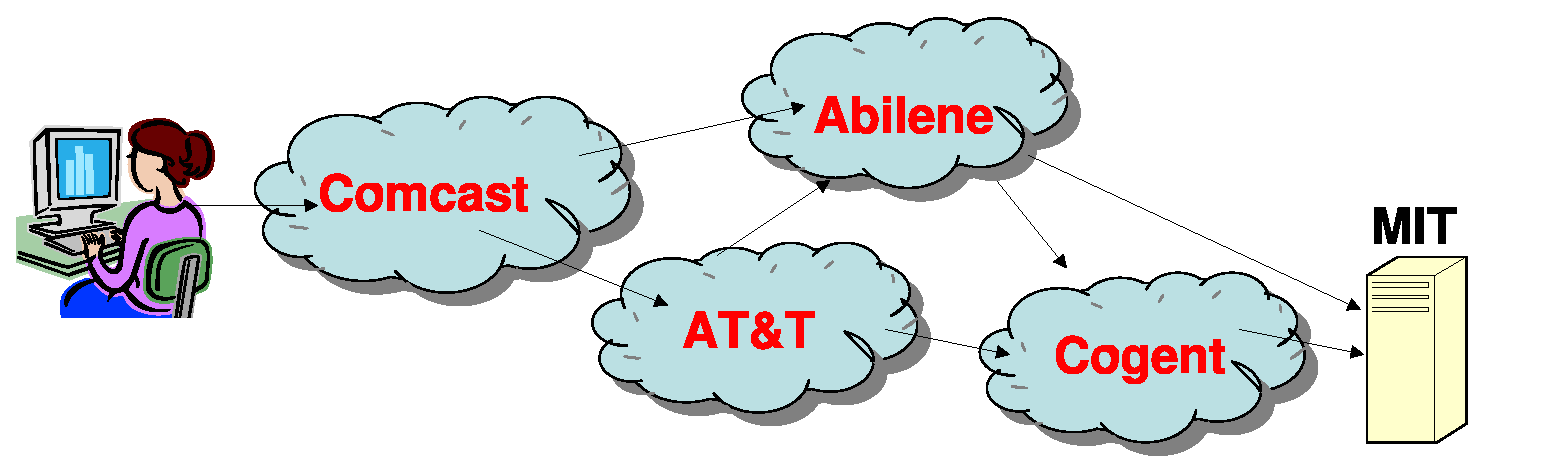
\epsfig{file=figures/overview.eps, width=\linewidth}
\caption[Overview of the Internet's structure]{A typical Internet path may traverse multiple ``Autonomous Systems''.}
\label{fig:intro:overview}
\end{figure}

\begin{figure}[t]
\centering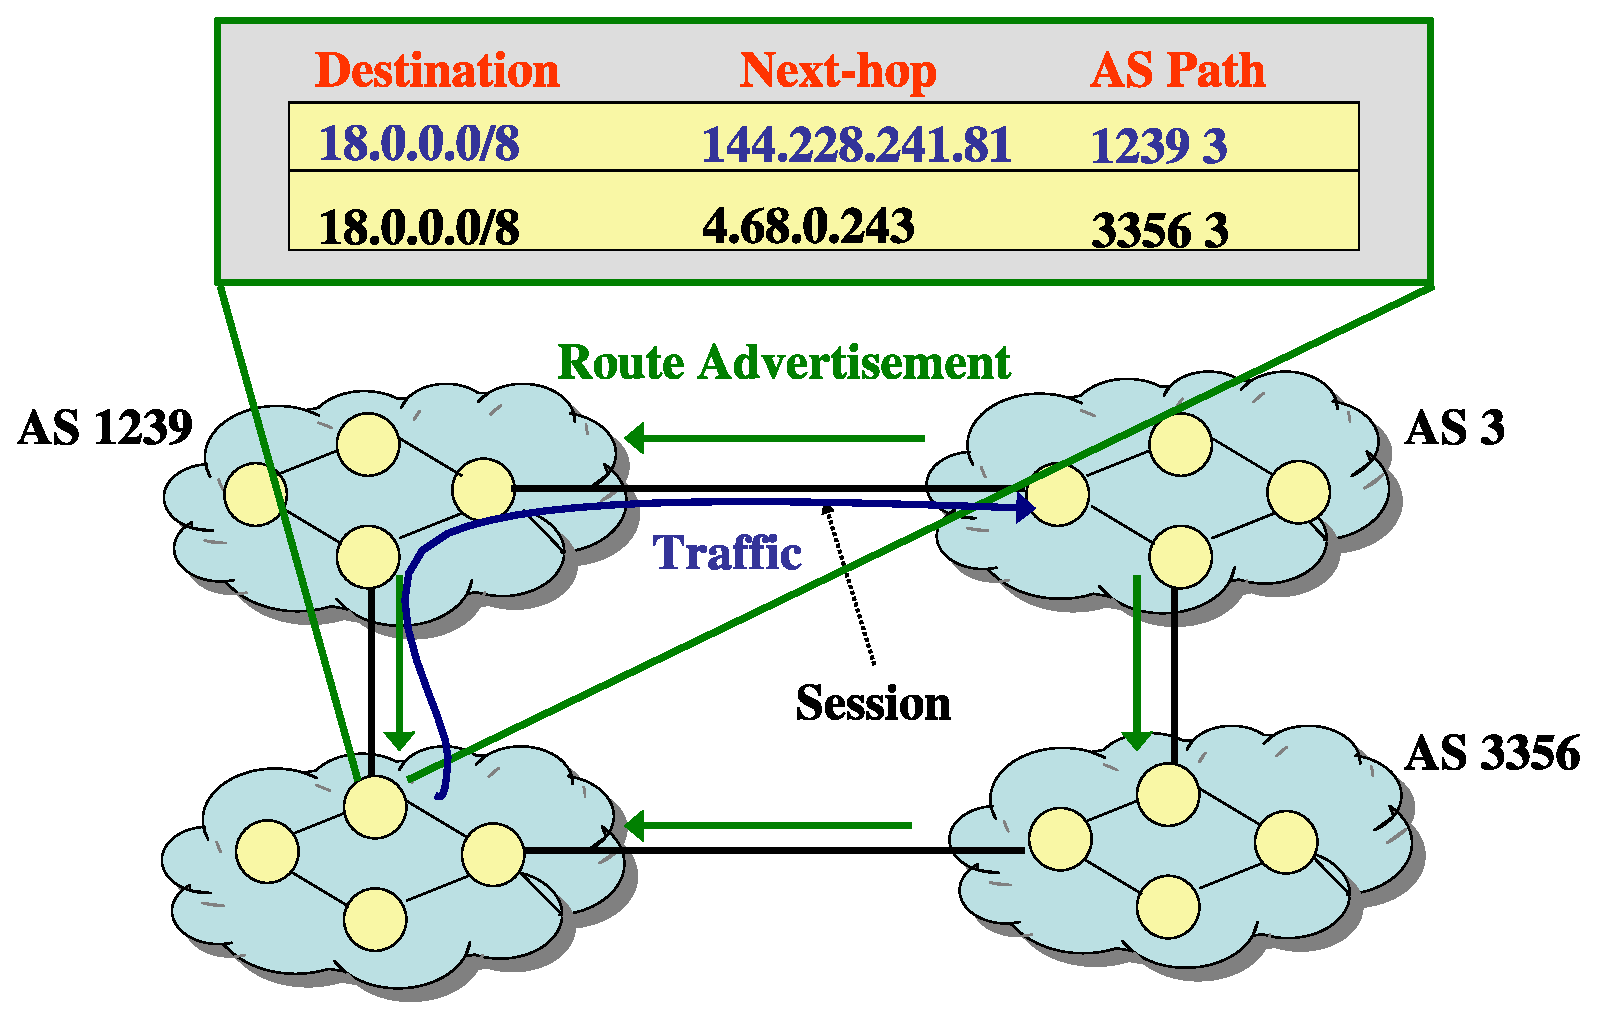
\epsfig{file=figures/rtgtable.eps, width=0.8\linewidth}
\caption[How ASes exchange routing information]{ASes exchange routing
information over BGP {\em sessions} between 
  routers.  A router may learn multiple routes to the destination but
  ultimately selects a {\em single} best route.  Traffic flows in the opposite
  direction of route advertisements.}
\label{fig:intro:rtgtable}
\end{figure}



Although it is common to think of ``the Internet'' as a single, monolithic
network, it is actually composed of tens of thousands of independently
operated networks, commonly called {\em Autonomous Systems} (ASes).
Figure~\ref{fig:intro:overview} shows an example of how traffic from a cable
modem user may traverse multiple ASes en route to machines at MIT.
Internet traffic is forwarded from source to destination through a
sequence of {\em routers} in one or more ASes.  

Each one of these ASes typically has independent (and often
conflicting) economic and performance goals, yet these ASes must cooperate by
exchanging routing information to achieve global connectivity (\eg, to
allow a home user who buys service from his cable modem provider to
communicate with hosts that purchase connectivity from other ASes).
The current routing protocol on the Internet is the Border Gateway
Protocol (BGP)~\cite{rfc1771}.  As shown in
Figure~\ref{fig:intro:rtgtable}, ASes achieve global reachability by
establishing BGP sessions between neighboring ``border'' routers.  Each
AS has may have anywhere from a single router to hundreds of routers. 
%
Each of these routers maintains a {\em routing table}, which contains
one or more routes for each destination.  Each router
selects a single best route to each destination.  Routing on the Internet
is {\em destination-based}; that is, a router selects the next hop (\ie,
router) for which to forward traffic solely based on the destination IP
address of each packet.  The destination for a route is represented in
terms of an IP {\em prefix}, which specifies a group of IP addresses
that share a common number of bits.


\begin{figure*}[tb!]
\begin{center}
\begin{small}
\begin{minipage}{5in}
\begin{verbatim}
   Network          Next Hop            Path
*> 18.0.0.0/8       144.228.241.81      1239 3 
*  18.0.0.0/8       12.0.1.63           7018 3356 3 
\end{verbatim}
\end{minipage}
\end{small}
\end{center}
\caption[Example BGP routing table entry]{BGP routing table entry for
prefix 18.0.0.0/8 as 
  it might appear on a router.  Each BGP route has attributes in
  addition to the next hop IP address and AS path, which we will discuss
  later.}
\label{fig:bgpex}
\end{figure*}


Figure~\ref{fig:bgpex} shows example routing table entries for the set
of destinations represented by the IP prefix {\tt 18.0.0.0/8}, which
represents the $2^{24}$ IP addresses that share the first 24 bits, {\tt
18.*}.  Although each router may learn multiple candidate routes
to a prefix, (\ie, the routing table shown in Figure~\ref{fig:bgpex} has
two possible routes for the same destination), each router ultimately
selects a {\em single} best route for each prefix (in the routing table,
the route that the router ultimately selects is indicated by the ``{\tt
>}''.  The {\em next hop} attribute is the IP address that the router
must forward traffic towards to send traffic along this route.  The
router may learn how to reach this next hop IP address in one of several
ways: a ``static'' route may be hardcoded, the router might learn a
route via a routing protocol that is run inside the AS (\eg, OSPF),
and so forth.  The {\em path} attribute refers to the AS path: the
sequence of ASes that the route advertisement traversed en route to this
router.  
%``Metric'' and ``LocPrf'' refer to the Multiple Exit
%Discriminator (MED) and Local Preference attributes, respectively; an
%operator can manipulate these two attributes to control which route a
%router ultimately selects, given multiple options.  
A BGP route has several additional route attributes that are not
pictured; we will describe
these additional attributes in more detail in Section~\ref{sec:propagation}.

Internet routing requires neighboring ASes to exchange routing
information, but it also requires each of these ASes to run an internal
routing protocol (``Interior Gateway Protocol'', or {\em IGP}) to
establish reachability information about destinations within the same
AS.  For example, in the routing table excerpt shown in
Figure~\ref{fig:bgpex}, the router knows that to forward traffic to any
destination in {\tt 18.*}, it must send the traffic towards the next hop
{\tt 144.228.241.81}.  For ``border'' routers, this next hop is typically
the address of an interface of the router in a neighboring autonomous
system and is an immediate next hop.  Routers within an AS, however,
must use the IGP to discover the outgoing
interface over which to send traffic towards this next hop, which may be
multiple hops away.  This dissertation focuses on BGP but does
not address the operation of internal routing protocols.  Other
work provides more detailed treatment of IGPs~\cite{Feldmann2001,
Shaikh2002, Shaikh2004}.


\section{Configuration: The Achilles' Heel of Internet Routing}
\label{sec:intro:config}

Analyzing the behavior of any routing protocol is inherently difficult,
but Internet routing presents a unique set of challenges because it must
be highly configurable to support the complex economic and performance
goals that each independently operated network is attempting to satisfy.
The standards document for BGP~\cite{rfc1771} specifies the message
format but intentionally leaves unspecified many details, including the
criteria for 
selecting the route to a destination given multiple alternatives.
Instead, these details are left to its {\em configuration}.  In this
section, we 
explain how configuration affects routing protocol behavior; we then
present some examples that demonstrate how configuration mistakes can
induce catastrophic routing failures.

\subsection{How Configuration Affects Routing Protocol Behavior}
\label{ssec:intro:config}

Internet routing configuration provides a network operator remarkable
latitude in controlling how the protocol behaves.  In particular,
Internet routing configuration allows an operator to control the routing
protocol in the following ways:

\begin{itemize}
\item {\bf Which ASes to carry traffic for.}  Depending on the
  business relationships that an AS has established with other
  ASes, it may arrange to carry traffic to a destination for some of
  those ASes but not others~\cite{Gao2001a}.  Routing configuration
  controls which routes an AS advertises to each of its neighbors,
  implicitly controlling which neighbors can send traffic over the
  AS en route to a destination.

\item {\bf How traffic enters and leaves the AS.} An AS
  typically has multiple links over which it can send traffic to a
  destination: some of these links are internal (\ie,
  they are between two routers in the same AS) and others are
  external (\ie, they are between routers in neighboring ASes).
  Changes in traffic demands may cause any of these links to become
  congested.  In response, a network operator may change the routing
  configuration to shift portions of the traffic load to a different set
  of links~\cite{Feamster2002b}. 

\item {\bf How routers within an AS learn routes to external
  destinations.}  Each independently operated network comprises tens to
  hundreds of routers.  Ultimately, every router in the AS must
  learn the routes to external destinations, but, initially, only the
  AS's ``border'' routers learn these routes.  Routing
  configuration controls how the routes propagate from an AS's
  border routers to the rest of the routers in the AS.
\end{itemize}


Changing traffic demands and business relationships, planned
maintenance, and equipment failures may all change traffic patterns
through the AS, but routing protocols do not automatically adapt to
these changing conditions.
As a
result, network operators must constantly tune the behavior of the
routing protocols in their ASes to control how traffic flows through
them.  

\subsection{Problem: Configuration Mistakes Cause Routing Failures}
\label{sec:intro:problem}

The cost of Internet routing's
configurability is a high degree of complexity.  The unfortunate
consequence of this complexity is that the potential for incorrect
behavior is enormous.

The consequences of incorrect behavior can be staggering.  The past few
years alone have seen several high-profile examples of Internet routing
configuration problems:

\begin{itemize}
\item In
1997, a small ISP in Florida configured its routing in a way that caused
all of the Internet's traffic to be routed through it~\cite{www-as7007}.
\item In 2001, Microsoft brought down its Web servers with a routing
misconfiguration; it took nearly a day to diagnose the
problem~\cite{www-microsoft-outage}.  
\item In 2002, Worldcom took down more
than 20\% of its nationwide ``backbone'' in the United States with a
routing configuration problem~\cite{www-worldcom-outage}.  
\item In 2004, Level3 incurred a widespread outage due to a router
configuration problem~\cite{www-l3-outage}.
\item In 2005, an ISP in Bolivia caused a major outage when it announced
the IP prefix for AT\&T's United States backbone
network (\ie, {\tt 12.0.0.0/8}).~\cite{nanog-att}. 
\end{itemize}
Major news outlets report only the most catastrophic routing failures;
in fact, mistakes in routing configuration are continually causing
reasonably serious routing failures.  In the introduction to
Chapter~\ref{chap:rcc}, we 
present the results of our informal study of the mailing list archives
of the North American Network Operators Group (NANOG)~\cite{nanog-list}.
In this study, we 
find that upwards of two-thirds of the routing failures reported on this
mailing list can be attributed to problems with routing configuration.
Network operators are continually misconfiguring routing protocols in
ways that cause such problems as loops, ``blackholes'' (where a router
simply drops traffic en route to some destination because it does not
have a route for it), routing instability, and so forth.  

%%%%%%%%%%%%%%%%%%%%%%%%%%%%%%%%%%%%%%%%%%%%%%%%%%%%%%%%%%%%

\section{Challenges}\label{sec:challenges}

While guaranteeing correct and predictable behavior poses challenges for
any routing protocol, Internet routing presents several unique
challenges.  First, Internet routing has more configurable facets
than traditional routing protocols, many
of which can be misconfigured or otherwise cause the routing protocol to
behave unpredictably.  In order to analyze the correctness of the
routing protocol, we must first define a specification for correct
behavior.  Second, the sheer size of the distributed
router configuration, as well as the fact that the configurations have
dependencies across routers, can give rise to erroneous or unpredictable
behavior.  Third, because each network operator configures his AS
independently of others, the policies defined in one AS may conflict
with those in neighboring ASes.

\subsection{Defining a Correctness Specification}

As described in Section~\ref{ssec:intro:config}, Internet routing
configuration affords a network operator much flexibility in defining
how the protocol operates.  The Cisco configuration language has more
than 1,000 different commands, and a network of 500 routers may have
upwards of one million lines of configuration distributed across the
AS~\cite{www-cisco-ios-master}.  Given the many ways in which an
operator can affect protocol behavior, determining the correctness of
the configuration is a daunting task without a high-level specification
for ``correct'' behavior.  Developing such a specification involves
distilling the high-level properties that the protocol should satisfy
from the protocol's mechanistic detail.

Defining a correctness specification for Internet routing is complicated
by the fact that the protocol's correctness is in part 
based on whether it achieves a network operator's economic
and performance goals.  Unfortunately, these high-level policies are
encoded in terms of mechanistic configuration commands distributed
across hundreds of routers---that is, the specification of the {\em
intended} behavior doesn't even exist in the first place, which makes it
difficult to determine whether the routing configuration indeed induces
the intended behavior.

One motivation for developing a correctness specification for Internet
routing is that the protocol not only ``does the right thing'' when it
satisfies the specification, but a routing protocol that satisfies the
specification is also more predictable.  For example, network operators
often would like to predict the effects of a configuration change on the
behavior of the routing protocol without testing that change on a live
network or running a complex simulator.  Predicting how the protocol
will behave first requires making assumptions about its behavior to
simplify route prediction, but precisely determining the constraints that
are required to simplify route prediction for such a complex protocol is
challenging.

\subsection{Analyzing Complex Configuration}

%% Configuring a network's routing boils down to independently configuring
%% the routers within a network.  Each network contains as many as several
%% hundred routers; each of these routers may have tens of thousands of
%% lines of configuration.  Although an operator configures each of these
%% routers separately, the configuration typically has dependencies across
%% multiple routers in the network.  Furthermore, a network may contain
%% routers from different vendors, each of which have a different
%% configuration language.  The configuration of these routers collectively
%% dictates the behavior of the network. In this sense, configuring a
%% network of routers is not unlike writing a large distributed program in
%% several different flavors of assembly language.  Given this complexity,
%% it is not surprising that network operators make mistakes in configuring
%% routers.

In designing tools that can help network operators reason
about the correctness of Internet routing, we must also design ways
to manage routing configuration's staggering complexity.  First, we must
represent this 
distributed router configuration in a format that is easy to analyze.
Second, we must tackle the engineering problem of parsing the various
routing configuration languages from different vendors and translating
the configurations into this format.

Determining how a configuration change will affect routing is difficult
in practice.  Not only do ASes contain a large number of routers, but
the route that each router ultimately selects for each destination
depends on many factors, including the routes that the AS's ``border''
routers learn from neighboring ASes, the routing topology within the AS
(\ie, both the internal topology, and the internal BGP topology that
controls how routes are disseminated within the AS).  As we discuss in
more detail in Chapter~\ref{chap:sandbox}, various complicating
protocol artifacts prevent informally reasoning about the route that each
router selects.  Thus, network operators need tools and
systematic techniques to assist them in predicting how a particular
routing configuration will affect the flow of traffic through the AS.


\subsection{Providing Global Guarantees with Only Local Information}

While end-to-end connectivity between Internet hosts fundamentally
depends on the {\em global} behavior of the routing system, no single party
has a global view of the Internet routing system. A network operator may
configure the protocol in a way that interacts in unexpected ways with
the configurations in other ASes.  For example, the interactions of
routing policies in neighboring ASes can cause the routing protocol to
oscillate.

One goal of our work is to explore how we can achieve assurances about
the global behavior of the Internet routing system, while still
preserving the {\em autonomy} of each AS.  That is, each network operator
should retain the ability to independently configure his own AS,
but should also be able to gain some assurances about the global behavior of
the routing system, assuming every AS abides by a similar set of
rules.  


%%%%%%%%%%%%%%%%%%%%%%%%%%%%%%%%%%%%%%%%%%%%%%%%%%%%%%%%%%%%


\section{The Role of Proactive, Static Configuration
Analysis}\label{sec:proactive}  

\begin{figure}[t]
\centering\epsfig{file=figures/workflow.eps, width=0.7\linewidth}
\caption[The state-of-the-art in network configuration management]{The state-of-the-art in network configuration management: {\em
reactive}, ``stimulus-response'' mode of operation.}
\label{fig:intro:workflow}
\end{figure}

Prior to our work, the state-of-the-art in managing Internet routing
protocols was {\em reactive}: the primary way for network operators to
determine the effects of a particular routing configuration (\ie, what
effects that configuration will have on the flow of traffic, or whether
the configuration is even correct in the first place) was to deploy that
configuration on a live network, observe the resulting behavior, and
revert the configuration to a previous version in the event that the
configuration did not produce the desired effects (see
Figure~\ref{fig:intro:workflow}).  This mode of operation has two
shortcomings: First, testing configuration on a live network can cause
unnecessary downtime or poor network performance (and, hence, angry
customers!).  Second, the undesirable effects that result from a
particular configuration may not be immediately apparent when the
configuration is deployed; a failure may only be triggered by the
presence or absence of certain routes.

This dissertation posits that {\em proactive} techniques for analyzing
routing configuration can both prevent a large class of routing failures
and help operators predict and analyze routing protocol behavior.
Changing the workflow from Figure~\ref{fig:intro:workflow} to include a
step that proactively detects problems with routing configuration is
critical for improving the correctness and predictability of Internet
routing.  A remarkable result of our work is that proactive analysis
techniques (\ie, those that analyze the static routing configuration
offline, before it is deployed on a live network) are useful in
detecting configuration faults and efficiently and accurately predicting
the routing protocol's behavior.  In particular, proactive analysis
techniques provide the following benefits over the status quo:

\begin{enumerate}
\itemsep=-1pt
\item {\bf Offline.}  A reactive mode of configuration is time consuming
and can lead to unnecessary performance degradation.  The complexity of
Internet routing makes it essentially impossible to compute
back-of-the-envelope estimates of the effects of configuration changes.
Proactive techniques for determining the correctness and the effects of
Internet routing configuration can help network operators evaluate the
effects of a routing configuration before it is deployed on a live
network.

\item {\bf Accurate.}  Network simulators (\eg,
ns~\cite{www-ns-bgp}, SSFNet~\cite{www-ssfnet}) help operators
understand dynamic routing protocol behavior, but simulation models
network behavior in terms of its protocol dynamics over some certain
period of time.  The {\em outcome} of the simulator will ultimately be
the same as that predicted by static techniques, and the dynamics (which
are nondeterministic) may not necessarily correspond to those in the
actual network anyhow.  Existing simulators do not capture all of the
relevant protocol interactions that may affect correctness, nor do they
explain {\em why} a particular configuration is incorrect.  Because
incorrect behavior sometimes depends on a particular sequence of route
advertisements or may be nondeterministic, correct behavior in a
simulator cannot guarantee correct behavior on a live network.  In this
dissertation, we show that techniques based on direct analysis of static
configuration files can test for necessary or sufficient correctness
conditions and predict the outcome of the routing protocol without
having to simulate the protocol dynamics.

%% While simulators can
%% prove useful, they are often unnecessarily complex: simulators can help
%% an operator study the {\em dynamics} of the network, but operators
%% typically do not care about such dynamics; rather they need to quickly
%% evaluate the {\em outcome} of the route selection process.


\item {\bf Efficient.}  Because network operators cannot use ``back of the
envelope'' calculations to determine what a particular routing
configuration will do, they must often experiment with many
possibilities before arriving at an acceptable solution.  As we will
show in Chapters~\ref{chap:rcc} and~\ref{chap:sandbox}, static analysis
techniques can assist network operators in efficiently determining the
correctness and effects of incremental changes to a routing
configuration.


\end{enumerate}

%% This dissertation presents techniques for determining both the
%% correctness and the outcome of this computation (1)~efficiently, (2)~in
%% a way that facilitates evaluating incremental changes, and (3)~without
%% having to observe the protocol's behavior on a live network.

Analyzing the static router configurations of a single AS proves
surprisingly effective at improving the correctness and predictability
of Internet routing.  An important open question that is {\em not}
addressed in this dissertation involves
exploring the classes of faults that {\em cannot} be detected with
static analysis alone and how analysis of routing {\em dynamics} might
complement static configuration analysis for fault detection and diagnosis.

%% this dissertation also recognizes
%% the limitations of static analysis.  We explore how dynamic analysis of
%% routing protocol messages can complement static configuration analysis,
%% and even changes to the routing protocol and architecture itself.



%%%%%%%%%%%%%%%%%%%%%%%%%%%%%%%%%%%%%%%%%%%%%%%%%%%%%%%%%%%%

\section{Contributions}\label{sec:contributions} 

We now briefly overview the major contributions of this dissertation
before describing each in more detail.  A central contribution of this
dissertation is a formal correctness specification for Internet routing.
We use this specification to derive tests for configuration faults and
as the groundwork for efficient offline analysis of Internet routing.
Using this specification as a guide, we present the design and
implementation of two systems that use proactive configuration analysis
techniques to improve the correctness and predictability of Internet
routing.  The first, \rcc (``router configuration checker''), detects
faults in routing configuration. \rcc helps network operators eradicate
configuration faults before they cause catastrophic routing failures on
a running network. The second, the {\em routing sandbox}, efficiently computes
the routes that each router within a single AS ultimately select, using
only a static snapshot of the routing configuration and network state.
%The
%BGP sandbox allows an operator to experiment with configuration changes
%offline and determine whether a possible configuration change would have
%the desired effect, before deploying the change on a live network.

Because Internet routing inherently involves interaction between
multiple independently operated, competing ASes, some aspects of the
correctness 
specification are difficult to verify by only looking at the
configuration of a single AS in isolation.  In particular, it turns out
to be difficult to determine whether the routing protocol will converge
to a stable route assignment (a property defined as {\em safety} in
previous work~\cite{Varadhan1996}).  Traditional routing protocols
typically satisfy safety, but BGP's {\em policy-based} nature means that
the policies of neighboring ASes can interact to create oscillations.
This dissertation provides the first necessary conditions for
guaranteeing the stability of a policy-based routing protocol.  The rest
of this section discusses these contributions in more detail.

%% While analyzing the static router configurations of a single AS
%% proves surprisingly effective at improving the correctness and
%% predictability of Internet routing, this dissertation also recognizes
%% the limitations of static analysis.  We explore how dynamic analysis of
%% routing protocol messages can complement static configuration analysis,
%% and even changes to the routing protocol and architecture itself.
%% Specifically, we present the design of the Routing Control Platform
%% (RCP), a routing system that separates the route selection logic from
%% the routers themselves and can explicitly guarantee many aspects of the
%% correctness specification.


%This dissertation also makes practical contributions in the areas
%of network management and Internet routing design.  While the
%contributions to network management may prove more immediately
%applicable, we believe that the work more relevant to routing design
%will ultimately make Internet routing intrinsically more robust and
%predictable.  In other words, while network management tools are crucial
%to network operation, our ultimate goal should be to {\em design the
%protocol for manageability}.  Our contributions to routing protocol
%design are a step in the right direction towards this goal.

\subsection{A Correctness Specification for Internet Routing}

We define three high-level properties that a routing
protocol should satisfy. Essentially, all three aspects of this
correctness specification
reflect the following underlying principle: {\em a routing protocol
should propagate 
information that accurately reflects the properties of the underlying
network topology}.  The three properties are as follows:

\begin{itemize}
\item {\bf Route validity.}  If an endpoint learns a route to a
  destination, then that route should correspond to some path.  An
  example of a route validity violation would be a persistent forwarding
  loop: a router learns a route to some destination (\ie, a destination,
  and the next-hop IP address to which traffic should be sent for that
  route), but when it actually attempts to send traffic along that
  route, it is caught in a forwarding loop and never reaches
  the destination.

\item {\bf Path visibility.}  If there exists a sequence of IP-level
  hops (\ie, a {\em path}) from an endpoint to a destination, then
  that endpoint should learn at least one route to that destination.  An
  example of a path visibility violation would be a case where all
  routers inside a fully-connected AS did not learn a route to the
  destination when at least one of those routers learned the route.  

\item {\bf Safety.}  This property requires that the
  routing protocol ultimately assigns a route to each node in the
  Internet graph 
  such that no node has a more preferred available route to the
  destination that it would rather use.  Safety is important not only
  because a routing protocol that persistently oscillates can cause lost
  and reordered packets, but also because it is incredibly difficult to
  diagnose problems when the routing protocol is changing independently
  of the underlying topology.  A violation of safety would be an
  oscillation caused by conflicting policies from different ASes (rather
  than due to topological changes), as described in previous
  work~\cite{Griffin2002c, Varadhan1996}.
\end{itemize}

Chapter~\ref{chap:rlogic} formalizes each of these
properties, as well as well as other concepts (\eg, path,
route, etc.).  Path visibility and route validity are violated primarily
because of configuration complexity, and safety is violated because the
configurations of one AS may interact in unexpected ways with
configurations of other ASes.

Although this dissertation applies this correctness specification to
Internet routing, these properties should prove valuable for analyzing
any routing protocol.  Applying these properties to routing in other
areas (\eg, wireless or sensor networks) is beyond the scope of our
work, but is ripe for exploration.

\subsection{Systems for Proactive Fault Detection and Route Prediction}

This dissertation recognizes a critical missing piece in the {\em
workflow} of configuring today's networks: the step at which network
operators evaluate the effects of a routing configuration before
deploying and running it on a live network.


\begin{figure}[t]
\centering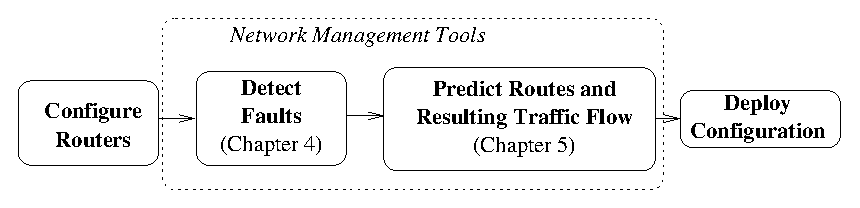
\epsfig{file=figures/workflow2.eps, width=0.75\linewidth}
\caption[This dissertation's contributions in fault detection and
route prediction.]{This dissertation develops two tools for fault detection
  and route prediction.  These tools should be used to analyze the
  behavior of routing configuration before it is deployed on a live
  network.}
\label{fig:intro:workflow2}
\end{figure}


\begin{figure}[t]
\centering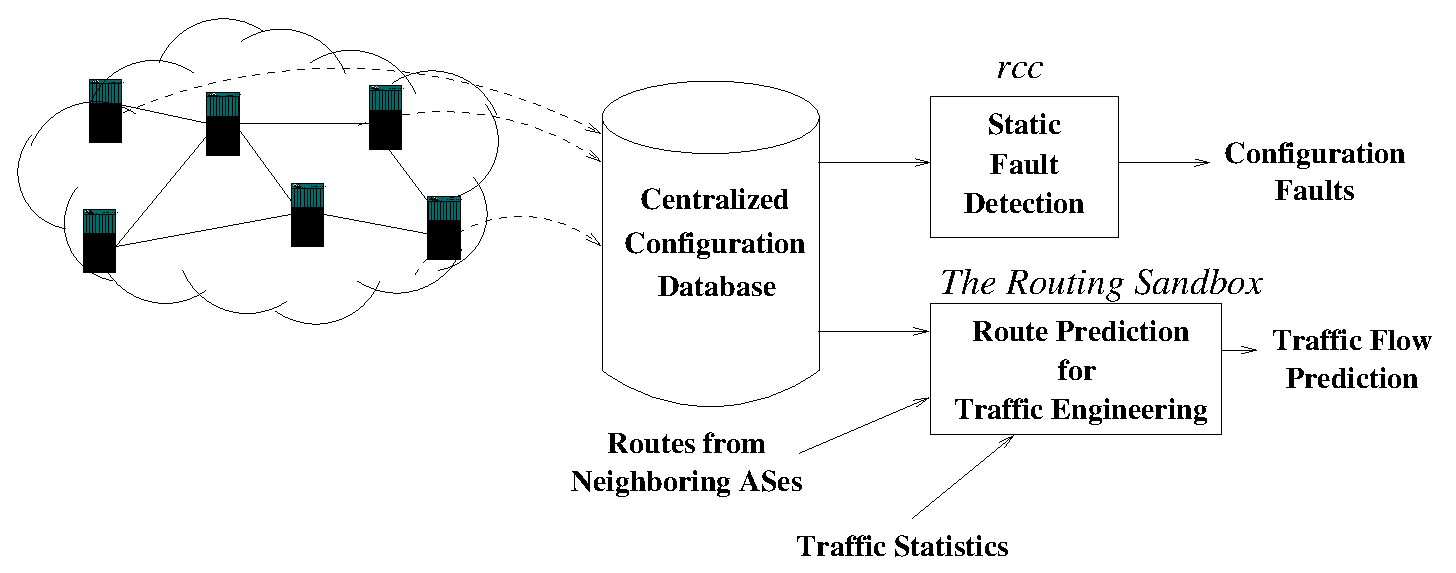
\epsfig{file=figures/process.eps, width=0.9\linewidth}
\caption[Workflow for fault detection and route prediction
  tasks.]{Workflow for fault detection and route prediction tasks 
  described in this dissertation. Both fault detection and route
  prediction tasks rely on {\em offline} analysis of the distributed 
  router configurations, which are first collected into a centralized
  database.}
\label{fig:intro:process}
\end{figure}


This dissertation presents two complementary systems that advance the
state-of-the art in fault detection and traffic engineering,
respectively.  Figure~\ref{fig:intro:workflow2} shows how these two
systems change the workflow of configuring routers.  Both of these new
systems analyze the {\em static} router configuration files.  We first
describe \rccns, a fault detection system for router configurations.  We
then describe the {\em routing sandbox}, a tool that predicts how traffic
will flow through an AS, given only a static snapshot of the router
configurations.  Together, these contributions assist a network operator
in detecting faulty routing configurations and determine the effects of
a configuration on traffic flow.

Because the techniques we present predict the behavior of the routing
protocol before it even runs, the techniques we present directly analyze
of the static configuration files.  Figure~\ref{fig:intro:process}
illustrates this process.  The configurations from the routers within an
AS are first collected from the routers and stored in a central
database.  Fault detection is performed by executing queries directly
against this repository (Chapter~\ref{chap:rcc} provides more details).
Route prediction for traffic engineering (Chapter~\ref{chap:sandbox}) is
performed in a similar fashion, but also requires additional inputs:
computing the routes that each router selects requires knowing which
routes each router learns from neighboring ASes in the first place.
Once the route that each router ultimately selects is computed, an
operator could use traffic statistics to determine the utilization on
each link in the network, but this dissertation does not address this
problem.

\subsubsection{\rccns: Proactive fault detection for Internet routing
configuration}

Chapter~\ref{chap:rcc} presents the design and implementation of \rccns,
the ``router configuration checker'', a tool that uses static 
configuration analysis to detect faults in the routing configurations
within a single AS.  We designed \rcc starting with the correctness
specification as a guide and determining the constraints on the 
aspects of configuration (described in more detail in
Section~\ref{sec:semantics}) that must hold to guarantee that the
higher level correctness properties are satisfied.  \rcc analyzes the
set of router configurations from a single AS and determines whether
they could induce violations of the correctness specification.  

{\em rcc} has been downloaded by over seventy network operators, and we
have personally used {\em rcc} to study faults in the
routing configurations of $17$ real-world ASes.
Chapter~\ref{chap:sandbox} presents algorithms and a tool that helps
network operators predict how a particular routing configuration will
affect the flow of traffic through the AS.  In conjunction with
{\em rcc}, this tool allows a network operator to answer critical
questions about routing configuration (\ie, whether the configuration
will cause catastrophic problems, and how it will affect the flow of
traffic through the AS) {\em before} the configuration is actually
deployed on a live network.

Our work on \rcc demonstrates that static configuration analysis can
detect a significant number of configuration faults that could cause the
routing protocol to violate correctness. Surprisingly, \rcc also
discovered many such faults in {\em deployed} routing configurations,
even those from large, well-known Internet service providers.  \rcc even
found configuration faults in ASes that use ``automated''
configuration techniques: of course, automated configuration systems
will have difficulty generating correct configuration if they do not
receive correct input in the first place.  Many of the
configuration faults that \rcc detects in practice suggest that
configuring a network 
of routers without introducing inconsistencies across router
configurations is surprisingly difficult.

%% Although \rcc uses only static analysis of routing configuration to
%% detect faults, some routing faults are best detected using analysis of
%% routing protocol dynamics in concert static configuration analysis may
%% also prove useful for detecting routing faults.  In
%% Chapter~\ref{chap:concl}, we speculate on scenarios where dynamic
%% analysis may prove useful.

\subsubsection{The Routing Sandbox: Proactive route prediction for
network engineering}

Chapter~\ref{chap:sandbox} describes algorithms that compute the effects
of a configuration change offline, given only a static snapshot of the
routing configurations and the available routes.  These algorithms can
then be combined with information about traffic demands to help network
operators determine how a particular routing configuration will affect
the flow of traffic through the AS.  Rather than simulating complex
protocol dynamics to determine the effects of configuration on route
selection, we model the {\em outcome} of BGP's route selection process.
{\em We exploit the properties of the correctness specification to
simplify this process:} assuming that \rcc has already verified that the
configuration satisfies route validity, path visibility, and safety
makes it possible to model AS-wide route selection without simulating
the dynamics of the routing protocols.

Route prediction becomes increasingly difficult in ASes that enable two
protocol ``features'': the Multiple Exit Discriminator (MED) attribute
and route reflection, which are described in
Sections~\ref{sec:propagation} and~\ref{sec:dissemination}, respectively.
We design algorithms for predicting BGP 
route selection for ASes that have any combination of these two features
enabled.  We also perform a running-time analysis of each of these
algorithms, which provides insight into how each of these features adds
complexity to Internet routing.

We have implemented these algorithms in a tool called the {\em routing
sandbox} that allows a network operator to {\em quickly} evaluate the
effects of incremental configuration changes.  This tool exploits
several unique aspects of the system inputs to optimize the computation
of routes for all destinations for every router in the AS.  We envision
that the routing sandbox could be used as an ``inner loop'' to other
tools that iteratively search through a large parameter space to find
optimal settings~\cite{Ye2003}.

\subsection{Conditions for Safety of the Global Routing System}



Configuration allows an operator to control both the route that each
router selects to a destination (\ie, {\em ranking}) and which routes
each router readvertises to neighboring routers (\ie, {\em filtering}).
One way to guarantee safety is to restrict some aspects of the
configuration's flexibility.  In Chapter~\ref{chap:policy}, we derive
necessary and sufficient conditions on the policies of each AS that
guarantee safety
if each AS independently follows these constraints.  Specifically, we
explore how each AS 
must restrict rankings to guarantee that the global routing system
satisfies safety, assuming that no AS wants to share its rankings with
any other AS, and no AS's rankings should be constrained by the rankings
of another AS (that is, each AS should retain {\em autonomy}).

We show that any protocol that does not restrict the business
arrangements of how ASes exchange routes with one another must impose
strong restrictions on how ASes are allowed to express preferences over
candidate routes for a destination.
%
Initially, this finding may sound rather grim, because shortest paths
routing may not provide network operators sufficient flexibility to
achieve their economic and performance goals.  On the contrary, the
results we present in this dissertation should be viewed as a first cut
towards designing routing protocols that are guaranteed to satisfy
safety, regardless of how they are configured.  Today, network operators
have no way to reason about the stability of the routing protocol, so
they are left to {\em ad hoc} methods for determining whether routing
updates correspond to unintended interactions.  A routing protocol that
conforms to the guidelines we outline in Chapter~\ref{chap:policy}
guarantees that changes in the routing protocol always reflect changes
in the underlying topology, thereby facilitating troubleshooting.
Furthermore, designing a protocol that is guaranteed to satisfy safety
on a fast timescale allows conflicts of business policy to be resolved
{\em outside} the protocol, rather than being reflected as oscillations
within the protocol itself.


\section{Lessons Learned}\label{sec:lessons}

This dissertation provides the following important lessons that can aid
the networking community as it considers proposals for evolving the
Internet routing infrastructure.

\subsection{Static configuration analysis detects many faults}

\rcc detected configuration faults in the routing configurations of all 17
ASes we analyzed and more than a thousand faults overall.  It may
seem surprising that \rcc was able to detect configuration faults in
{\em deployed} routing configurations.  In fact, this finding
demonstrates that there are many potentially catastrophic configuration
faults that do not immediately cause routing failures when they are
deployed.

The fact that static analysis can find important configuration faults
without overwhelming network operators with a vast quantity of false
positives is also somewhat remarkable.  \rcc does {\em not} operate with
a specification of the routing protocol's intended behavior.  Rather, it
operates solely on the routing configurations that {\em implement} an
operator's intent with low-level mechanisms.  Ideally, \rcc would check
the router configurations against a high-level specification of intended
behavior.  It is noteworthy that \rcc can provide a useful tool to
network operators in the absence of such a specification.

Configuration languages may ultimately evolve to make certain types of
configuration faults less likely, but static configuration analysis will
remain a crucial step in the workflow of network operations.  We believe
that the more mechanistic aspects of routing configuration will
ultimately be supplanted with high-level policy specification.  For
example, preventing routes that were learned from one neighboring
AS from being advertised to another today requires configuring
low-level, mechanistic operations on every router that exchanges routes
with either of those ASes.  Such a simple policy would better be
expressed in a specification language and ``compiled'' to the statements
that implement the mechanisms on the routers themselves.  However,
because Internet routing must always afford a network operator
flexibility in controlling the behavior of the protocol, static
configuration analysis will be invaluable for detecting faults and
evaluating routing protocol behavior, {\em
regardless of the configuration language}.  

\subsection{Distributed routing configuration leads to errors}

Our study of configuration faults in Chapter~\ref{chap:rcc}
(Section~\ref{sec:evaluation}) demonstrates
that most configuration faults result from the fact that routing
protocol configuration is {\em distributed} across the routers in the
AS.  This approach naturally causes operators to make mistakes because
it is more natural to think of the AS {\em as a whole} as implementing
some certain task (\eg, controlling traffic flow, implementing
contractual arrangements, etc.) rather than reasoning about what each
router must do to implement such a task.  A better approach may be to
allow operators to configure the AS as a monolithic entity from a
single location.

Of course, a crucial open research challenge upon which this goal
depends is what that centralized language should look like, and how the
routers themselves should implement the directives in that language.
Recent work in constraint satisfaction for network configuration
presents a possible starting point for a centralized configuration
language that satisfies high-level specification~\cite{Narain2004}.

A logically centralized routing infrastructure could act as
a catalyst for such a centralized configuration language.  For example,
a network operator could configure the AS from the RCP, which could
either (1)~compile this high-level specification into low-level router
configurations, and {\em push the configuration} to the individual
routers or (2)~select the routes on behalf of each router and {\em push
the routes} themselves to the routers.

\subsection{Safety + Autonomy $\Rightarrow$ Tight restrictions on
expressiveness} 

The (strict) conditions we derive in Chapter~\ref{chap:policy} for
guaranteeing safety suggest several possible ways for evolving the
Internet routing infrastructure.  One possibility is to relax the
autonomy requirement, by allowing groups of ASes to share certain
properties about their rankings with one another (although likely not the
rankings themselves).  Recent work has begun exploring this possibility
by recognizing that some ASes may have rankings that are more expressive
as long as others are not and designing ways to guarantee these global
properties without requiring ASes to divulge sensitive information about
rankings~\cite{Machiraju2004}.  One area for future work to determine
the information that must be shared (and with what other ASes it must be
shared) to detect and {\em resolve} safety violations, and, in
general, to study the tradeoffs between safety and the autonomy and
privacy of an ASes rankings.

Another possibility for evolving the Internet routing system is to
restrict expressiveness so that rankings must be consistent with
shortest paths routing, but allow each AS to control the weights on
edges incident to itself.  Such a routing protocol would always
satisfy safety (even assuming ASes are allowed to filter routes
arbitrarily), and any
%but the protocol may converge to a path assignment that a
%network operator does not want, hence causing the operators of each
%AS to repeatedly fiddle with rankings.  If a set of ASes have a
%legitimate policy conflict (\eg, a set of ASes all prefer routes through
%each other, thus creating a cycle of preferences), the protocol would
%then oscillate in accordance with network operators updating their
%rankings.  Such 
policy disputes could then be resolved with a negotiation protocol that
operates independently of the routing protocol, where routing updates
would only reflect actual changes in the network topology.  We explore
this possibility and others in detail in
Chapter~\ref{chap:policy} (Section~\ref{sec:policy:implications}).
 

\subsection{Protocol design should consider correctness and
predictability}\label{sec:mods} 

This dissertation focuses on improving the correctness and
predictability of the current Internet routing system, but a major
lesson from our work is that many of the tools and techniques that we
develop in the coming chapters could have been much simpler had the
protocol been designed with correctness and predictability in mind in
the first place.  

To this end, this dissertation proposes several minor modifications to
the Internet routing protocol that would have simplified the task of
achieving correct and predictable behavior.  These modifications are
minor in the sense that they can be implemented with no modifications to
routers or routing protocol specifications; on the other hand, they are
significant because they eliminate the artifacts that result from the
two most troublesome aspects of BGP: route reflection and the ``multiple
exit discriminator'' (MED) attribute.  In summary, we will see that
these two artifacts are responsible for much of the undesirable behavior
in Internet routing, ranging from persistent oscillation to network
partitions.  
%% In Chapters~\ref{chap:policy} and~\ref{chap:sandbox}, we will see that
%% much of the complexity of predicting the outcome of BGP route selection
%% is caused by route reflection, the MED attribute, and the interaction
%% between these two artifacts.  While MED serves a useful purpose in
%% allowing one AS to express preferences over exit points to its neighbor,
%% it also can create protocol oscillations, because the presence or
%% absence of some route can affect a router's relative preference between
%% two {\em different} routes.  This behavior arises because different
%% neighboring ASes may assign different MED values; as a result, a router
%% can only compare the MED values among routes from the {\em same} AS for
%% that destination, not across all routes for that destination.  In
%% Chapter~\ref{chap:sandbox} (Section~\ref{sec:sandbox:med_disc}), we
%% propose a small modification to BGP configuration that allows the MED
%% attribute to be compared across all routes to a destination (thus
%% eliminating the possibility for MED-induced oscillations) but still
%% preserves the ability for a neighboring AS to express relative
%% preferences over exit points.

One logical conclusion that can be drawn from the work in
this dissertation is that, rather than trying to {\em infer} the
protocol's behavior, the Internet routing system should provide more
direct {\em control} over route selection.
%
This insight is central to the Routing Control Platform (RCP) proposal,
which we describe briefly in Section~\ref{sec:rcp}.  RCP takes as input
the routes that an AS learns from neighboring ASes and the network
configuration, and computes routes on behalf of each router in the AS.
In some sense, RCP can be viewed as the logical extension to the routing
sandbox: RCP takes roughly the same inputs as the sandbox, but rather
than simply computing the routes that each router would select, RCP
actually controls route selection.

%% RCP
%% ensures that the route assignments for each router are based on a
%% complete view of the AS topology, and that routers are selecting paths
%% through the AS in a consistent fashion, thereby preventing forwarding
%% loops, blackholes (\ie, instances where traffic arrives at a router that
%% has no routing table entry for it), etc.  Recent work has demonstrated
%% that RCP can be used to perform route selection on behalf of all of the
%% routers in a large tier-1 ISP~\cite{caesar2004}, but many questions
%% remain.  Chapter~\ref{chap:concl} (Section~\ref{sec:rcp}) presents an
%% initial design of RCP and discusses the various benefits it could
%% provide (as well as open questions).

%\subsection{Eliminating MED while retaining its benefits} 





\section{How to Read This Dissertation}\label{sec:guide}

The problems with today's Internet routing infrastructure suggest one of
two attitudes:

\begin{enumerate}
\item Accept the Internet routing architecture ``as is'' and retrofit
  correctness and predictability by providing tools and techniques that
  make network operations less prone to faults and more predictable.
\item Adapt the routing architecture to make incorrect behavior
  less likely in the first place.
\end{enumerate}

Various parts of this dissertation cater to each of these philosophies.
The former philosophy can have more immediate impact and in fact can
provide ``bottom up'' insight regarding what aspects of the routing
architecture are most problematic.  Chapters~\ref{chap:rcc}
and~\ref{chap:sandbox} adopt this philosophy by providing tools and
algorithms that have helped network operators {\em today}.  \rcc has
been downloaded by over seventy network operators and has successfully
detected faults in the configurations of many large backbone Internet
Service Providers.  Additionally, the faults that \rcc uncovered in our
analysis of 17 real-world ASes, as well as the various aspects of BGP
that contribute complexity to the algorithms in
Chapter~\ref{chap:sandbox}, have helped us identify the aspects of the
routing architecture that beg for improvement.

Chapter~\ref{chap:policy} explores possibilities for improving routing
stability that will most likely require fundamental changes to the
Internet routing architecture because the conditions for stability would
require changing the configuration ``knobs'' that are exposed to network
operators.  The problems examined in this chapter use restrictions on
{\em static} configuration of the routing protocol to guarantee stable
dynamics.  
%% Section~\ref{sec:rcp} moves beyond simple static analysis,
%% proposing a fundamentally new mechanism for disseminating routes within
%% an AS and opening up new possibilities (as well as many unanswered
%% questions) for network management and configuration.

This dissertation caters both to the theoretician and the practitioner.
Chapter~\ref{chap:rlogic} presents a correctness specification for
Internet routing that could appeal to both parties.  Those most interested in
practical applications should focus primarily on Chapters~\ref{chap:rcc}
and~\ref{chap:sandbox}; Chapter~\ref{chap:policy} has fewer immediate
practical applications, but will be of interest to those interested in
fundamental results on routing stability and safety.  At the end of
Chapters~\ref{chap:rcc},~\ref{chap:sandbox}, and~\ref{chap:policy}, we
explore possibilities for 
evolving the Internet infrastructure to make the problems we solve
easier in the future; these sections should also have broad appeal.

%a thorough treatment (and
%hopefully lucid explanation) of Internet routing stability.

\setcounter{chapter}{1}
%\qchapter{\textit{You can observe a lot just by watching.} \vskip 0.1em
%  - Yogi Berra}{Related Work}

%"I don't compare 'em, I just catch 'em." - Willie Mays

%Leroy "Satchel" Paige: Quotations: Baseball
%Dont look back. Something might be gaining on you.

%\qchapter{I don't want to play golf.  When I hit a ball, I want someone
%  else to go chase it.  \vskip 0.1em - Rogers Hornsby}{Background and
%  Related Work} 
%\chapter{Related Work}

\qchapter{\textit{Don't look back.  Something might be gaining on you.}  \vskip
0.1em - Leroy ``Satchel'' Paige}{Background and Related Work} 
\label{chap:related}


\cs{I}n~this chapter, we provide an overview of how routing on the
Internet works today, as well as prior work on improving the correctness
and predictability of Internet routing.  We begin in
Section~\ref{sec:structure} with an overview of today's Internet routing
infrastructure: we describe the high-level organization of the Internet
(\ie, as a federation of thousands of independently operated networks
that exchange reachability information) and proceed to describe in
detail the routing protocols that these networks use to achieve global
reachability.
%Finally, in
%Section~\ref{sec:rw_architectures}, we discuss various proposals that
%involve making more fundamental changes or additions to the Internet
%routing architecture.
%
%In Section~\ref{sec:structure}, we describe the structure of the
%Internet and the operation of each independently operated network; we
%also briefly summarize the Internet's competitive landscape.
Section~\ref{sec:bgp} describes how these independently operated
networks exchange routing information with one another using the Border
Gateway Protocol (BGP)~\cite{rfc1771,id-bgp4}, and
Section~\ref{sec:conf} both explains at a high-level how configuration
controls BGP's operation and presents a brief example that describes
Cisco's router configuration language syntax~\cite{www-cisco-ios-master,www-juniper-command-ref}.
Section~\ref{sec:rw_challenges} presents an overview of previous studies
related to the correctness and predictability of Internet routing.
Readers who are already familiar with today's Internet routing protocols and
infrastructure (in particular, BGP) may wish to skip directly to
Section~\ref{sec:rw_challenges}.



\section{Internet Structure and Operation}\label{sec:structure}

Tens of thousands of independently operated networks connect to each
other to form the larger network that we know as ``the Internet''.
These networks are called {\em Autonomous Systems} (ASes), and they
cooperate with one another to provide global connectivity.
Nevertheless, these networks are also in {\em competition} with one
another.  Each one of these ASes contains many routers.  The routers
inside of one of these networks run an internal routing protocol called
an {\em interior gateway protocol} (IGP) that allows them to discover
routes to other destinations within the same AS, including the AS's {\em
border routers}---those routers that connect to neighboring ASes.
Examples of IGPs are Open Shortest Paths First (OSPF)~\cite{rfc1583},
Intermediate System-Intermediate System (IS-IS)~\cite{rfc1142}, and
Routing Information Protocol (RIP)~\cite{rfc1058}.

The Internet is composed of many different types of ASes, from
universities to corporations to regional Internet Service Providers
(ISPs) to nationwide ISPs.  Smaller ASes (\eg, universities,
corporations, etc.) typically purchase Internet connectivity from ISPs.
Smaller regional ISPs, in turn, purchase connectivity from larger
ISPs with ``backbone'' networks.  

The different types of ASes lead to different types of business
relationships, and, hence, different policies for exchanging and
selecting routes.  Although we will expound on these business
relationships later in this chapter, it is reasonable to think of these
business relationships in terms of two types: {\em customer-provider}
and {\em peering}.  Customer-provider relationships involve one AS (the
``customer'') paying another (the ``provider'') in exchange for carrying
its traffic to some portion of the Internet's destinations (often, every
destination outside of its own network)~\cite{Gao2001}.  In today's
Internet routing, 
{\em a route advertisement is an implicit agreement for carrying
traffic}.  The process of carrying traffic between two different ASes is
called ``providing transit''.  In these relationships, the customer pays
the provider for transit, regardless of the direction in which the
traffic is flowing.

In {\em peering} relationships, two ASes agree to trade traffic to
various destinations at no cost.  Typically, a pair of ASes will
recognize that it is more cost-effective to directly exchange traffic to
(some or all of) one another's customers, rather paying to send the
traffic through one or more provider ASes.  For those interested in a
more detailed treatment of the business aspects of peering, Norton
provides an excellent overview of peering and the decision parameters
that ASes must consider for deciding whether to peer~\cite{Norton2000}.


%%%%%%%%%%%%%%%%%%%%%%%%%%%%%%%%%%%%%%%%%%%%%%%%%%%%%%%%%%%%

\section{Internet Routing: The Border Gateway Protocol}\label{sec:bgp}

In this section, we describe the operation of the Border Gateway
Protocol, version 4 (BGP)~\cite{rfc1771,id-bgp4}.  The first two
sections describe the basic 
operation of the protocol---the protocol state machine, the format of
routing messages, and the propagation of routing updates---all of which
is defined in the protocol standard~\cite{rfc1771}.  A noteworthy aspect
of BGP is that many of the features that determine the behavior of the
global routing system are {\em not} standardized.  Later in this section, we
discuss two important non-standard aspects of Internet routing:
the route selection process and configuration languages.

To ensure reliable delivery of routing messages, all BGP sessions
exchange information using the Transmission Control Protocol
(TCP)~\cite{rfc793} 
(the same transport protocol used by common Internet applications that
require reliable message delivery, such as email and the Web).  Like
TCP, BGP also has a protocol state machine. Because BGP's state machine
is primarily concerned with enabling two routers to establish a
communication channel with one another and is unconcerned with the
routing messages themselves (all routing messages are exchanged in the
``{\tt ESTABLISHED}'' state), we forgo further description of BGP's
state machine.  For a detailed description of BGP's finite state machine
(including how timers can affect the transition between protocol states,
and when these timers are reset), see the protocol standard and related
documents~\cite{Beijnum2002, rfc1771, Stewart98}.


%% \begin{figure}
%% \centering\epsfig{file=figures/bgp_fsm.eps, width=0.3\linewidth}
%% \caption[BGP's finite state machine]{BGP's finite state machine.
%% Routing updates are exchanged 
%% between two routers that are in the {\tt ESTABLISHED} state.}
%% \label{fig:bgp_fsm}
%% \end{figure}

%% Figure~\ref{fig:bgp_fsm} provides an overview of BGP's finite state
%% machine and the messages exchanged between two routers to establish a
%% BGP session.  


%% Each router that runs BGP initially begins in the idle
%% state, and listens for connections on port 179.  A neighboring router may
%% then try to initiate a TCP connection to that router; when that router
%% attempts to establish a connection, it transitions to the {\tt CONNECT}
%% state.  If the connection succeeds, the router sends an {\tt OPEN}
%% message to its neighbor and transitions to the {\tt OPEN\_SENT} state
%% and waits to receive an {\tt OPEN} message from its neighbor.  If the
%% connection fails, the router returns to the {\tt ACTIVE} state,
%% whereupon it will listen for connections on port 179, wait for a retry
%% timer to expire and re-attempt to establish a TCP connection
%% (transitioning again to the {\tt CONNECT} state).  
%% %
%% Upon receiving an {\tt OPEN} message from its neighbor in the {\tt
%% OPEN\_SENT} state, the router checks the message for correctness.  If
%% the message is not correct, the router will send a {\tt NOTIFICATION}
%% message, close the connection, and return to the {\tt IDLE} state.  If
%% the message has no errors, the router sends a {\tt KEEPALIVE} message
%% back to the router that sent the {\tt OPEN} and changes its state to
%% {\tt OPEN\_CONFIRM}, where it waits for either a {\tt KEEPALIVE} or {\tt
%% NOTIFICATION} from the neighboring router.  If the router receives a
%% {\tt KEEPALIVE}, it then transitions to the {\tt ESTABLISHED} state;
%% otherwise, it returns to the {\tt IDLE} state.

%% The {\tt ESTABLISHED} state is the state of the protocol that the
%% routers are in when BGP is in its normal mode of operation---that is,
%% when it is exchanging routing {\tt UPDATE} messages (which we will
%% henceforth simply call {\em updates}).  The next section describes these
%% routing updates in more detail.  In the {\tt ESTABLISHED} state, routers
%% also exchange {\tt KEEPALIVE} messages to indicate that the link between
%% the two routers is still operational (since TCP provides no such monitoring
%% capability).


\subsection{Route Propagation: Announcements and
Withdrawals}\label{sec:propagation} 

\begin{table}
\begin{tabular}{l|p{3.45in}}
{\bf Route Attribute} & {\bf Description} \\ \hline
{\em Next Hop} & 
\parbox{3.45in}{
\vspace*{0.05in}
IP Address of the next-hop router along
the path to the destination. \\ On eBGP sessions, the next hop is set to
the IP address of the border router. On iBGP sessions, the next hop
is not modified.
\vspace*{0.05in}
} 
\\ \hline
{\em Multiple-Exit Discriminator (MED)} & 
\parbox{3.45in}{
\vspace*{0.05in}
Used for comparing two or more
routes from the same neighboring AS.  That neighboring AS can set the
MED values to indicate which router it prefers to receive traffic for
that destination. \\ {\em By default, not comparable among routes from
different ASes.}
\vspace*{0.05in}
} 
\\ \hline
{\em Local Preference} & 
\parbox{3.45in}{
\vspace*{0.05in}
This attribute is the first criteria used to
select routes.  It is not attached on routes learned via eBGP sessions,
but typically assigned by the import policy of these sessions;
preserved on iBGP sessions.}
\vspace*{0.03in}
\\ \hline
\end{tabular}
\caption{Commonly used BGP route attributes.}
\label{tab:route_attributes}
\end{table}

To understand how routers exchange routes using BGP, it is important to
keep in mind several defining features.  First, BGP is a {\em
path vector} protocol.  In a path vector protocol, routing updates
contain the sequence of ASes that the routing advertisement traversed
(\ie, the {\em AS path}).  BGP includes AS path information to avoid the
``counting to infinity'' problem that exists in traditional distance
vector protocols~\cite{Halabi2001}.  The AS path allows an AS that
learns a route to determine whether or not it has already heard the
route by checking to see whether its own AS is contained in the
path.\footnote{Contrary to what many believe, the AS path is {\em not}
intended to indicate the sequence of ASes that traffic will traverse en
route to the destination, although the AS path and this sequence of ASes
often match~\cite{Mao2003}.}  Destinations are represented
as IP {\em 
prefixes}, as described in Section~\ref{sec:intro:overview}.  A BGP
route announcement has several associated route attributes in addition
to the AS path, many of which are obsolete.  The most relevant BGP route
attributes are summarized in Table~\ref{tab:route_attributes}.


Second, BGP maintains state about the routing topology: routers do not
periodically ``refresh'' routing reachability information; rather,
routing messages reflect only {\em changes} in this information.  These
changes in information are reported with two types of routing updates:
{\em announcements} and {\em withdrawals}.  To announce that it can
reach a destination (or to change the existing route to a destination),
a BGP-speaking router sends an announcement for that destination to a
neighboring router.  If a destination is no longer reachable, a router
sends a withdrawal message to the neighboring router.  That neighboring
router may be located either in a neighboring AS or in the same AS.  BGP
sessions between routers in the same AS are called {\em internal BGP
(iBGP)} sessions, and those between routers in different ASes are called
{\em external BGP (eBGP)} sessions.  The goal of eBGP is to allow ASes
to exchange reachability to destinations in each other's networks; the
goal of iBGP is to ensure that {\em every} router within an AS learns at
least one route to every destination.


\subsection{Route Selection (And How Operators Can Control
It)}\label{sec:bg:route_selection} 

\begin{table}
\begin{small}
\begin{center}
\begin{tabular}{r|l|l} 
{\bf Step} & {\bf Criterion} & {\bf How Configuration Can Manipulate
This Step} \\ \hline
1 & Highest local preference & AS's import policy \\
2 & Lowest AS path length & Neighboring AS can ``prepend'' additional hops \\
{\color{Gray} 3} & {\color{Gray} Lowest origin type}   & {\color{Gray} Obsolete} \\
4 & Lowest MED (with {\em same\/} next-hop AS) & Neighboring AS's export
policy \\
5 & eBGP-learned over iBGP-learned  & ---\\
6 & Lowest IGP path cost to egress router & AS's IGP topology \\
7 & Lowest router ID of BGP speaker & --- \\
\end{tabular}
\end{center}
\end{small}
\caption{Steps in the BGP route selection process.}
\label{tab:background:decision}
\end{table}


Any given router may learn multiple routes to a destination (\ie, IP
prefix), but must ultimately select a single best route along which to
forward traffic to that destination.  The route selection process
determines which route each router selects.  The original standards
document does not specify the route selection process~\cite{rfc1771},
but the route selection process has since become a {\em de
facto} standard~\cite{www-cisco-bgp-path, id-bgp4}.

Table~\ref{tab:background:decision} summarizes the route selection
process, as well 
as how network operators can use routing configuration to try to
influence which route each router selects at each step of the process.
First, given multiple routes to the same destination (\ie, IP prefix), a
router will select the route with the highest ``local preference''
value.  As this attribute is not set by the receiving AS's import policy
and is the first step in the decision process, it provides the operator
direct influence over which route the router ultimately selects
to this destination.  Operators typically use the local
preference attribute to implement the types of policies described in
Table~\ref{tab:business}.  

\begin{figure}
\centering\epsfig{file=figures/prepend.eps, width=0.65\linewidth}
\caption[The use of AS path prepending to control inbound
traffic]{Operators sometimes use {\em AS path prepending} to try to 
control inbound traffic.}
\label{fig:prepend}
\end{figure}


Among multiple routes to a destination with equal local preference
values, a router will 
select the route with the shortest AS path length, which is simply
the number of AS-level hops in the AS path.  This criterion is 
a crude approximation for selecting a shortest path to the destination.
In practice, a
path with the fewest number of ASes does not correspond to the
path with the lowest latency, or to the path with the fewest number of
IP-level hops.  However, network operators do use routing configuration
to try to influence route selection using a technique called {\em AS
path prepending}, which artificially increases the length of a route's AS
path by adding the same AS number to the path multiple times.
Figure~\ref{fig:prepend} illustrates this practice: AS~1 wants inbound
traffic for $D$ to arrive via AS~2, rather than via AS~3.  To express
this preference, it
prepends an additional ``$1$'' to the AS path for its route to $D$ when
it advertises the route to AS~3.  If an upstream AS, say AS~4, learns
two routes to $D$---\ie, one via AS~2 and the other via AS~3---it will
prefer the route with the route via AS~2 because it has a shorter AS path
length (assuming it does not assign a higher local preference to routes
learned from AS~3).  Of course, this technique for controlling inbound
traffic has limited utility in practice, because AS~1 does not control
the policies (\ie, local preference values) of other ASes, and it also
cannot easily determine the AS path lengths that an upstream might see
for its route advertisements~\cite{Gao2005}.  Despite the fact that
prepending is widely used, the technique is largely ad hoc and of
only limited utility~\cite{Feamster2003e, Quoitin2005}.


If a router has two routes to the same destination with equal local
preference and AS path length, the router will then select the route with the
lowest ``origin type''.  Because this route attribute is deprecated, in
practice, 
route selection then typically falls to selecting the route with the
lowest multiple exit discriminator (MED) value.  If a neighboring AS
advertises a route to an AS at multiple locations, it may attach
different MED values to these routes to indicate that it prefers a
neighboring AS to use one exit point over another.  For example, in
Figure~\ref{fig:rw_med}, AS~1 is indicating to AS~2 that it wishes to
have traffic sent to destination $d$ via the exit point in New York
over the one in San Francisco by advertising the route to $d$ with a larger
MED value over the BGP session in San Francisco.  By default, the MED value is
only comparable among routes learned from the same neighboring AS, since
different ASes may use different ranges of MED values to specify
preferences over routes.  As we will see later in this dissertation, the
fact that the MED attribute is not comparable across all routes creates
many problems for correctness and predictability.

\begin{figure}
\begin{minipage}{0.48\linewidth}
\centering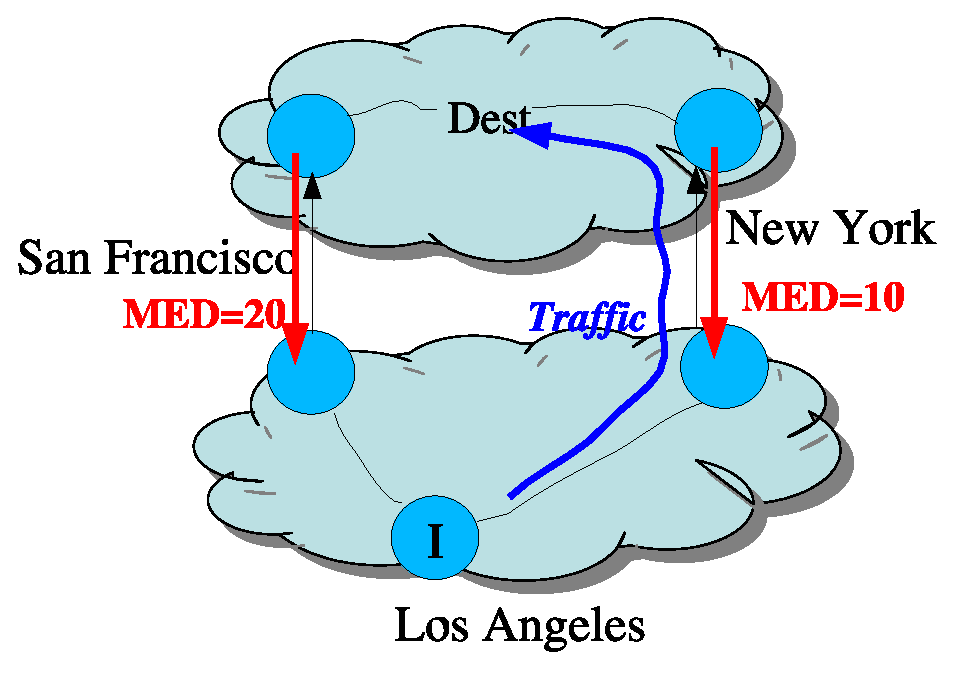
\epsfig{file=figures/med.eps, width=\linewidth}
\caption[The use of the MED attribute to control inbound traffic]{A
neighboring AS can advertise routes to a destination with 
different MED values at different locations to control the exit point
that routers in a neighboring AS uses to send traffic for that
destination.  When $I$ learns both routes, it will select the route
learned via the router in New York (and, thus, it will send traffic that
way).}
\label{fig:rw_med}
\end{minipage}
\hfill
\begin{minipage}{0.48\linewidth}
\centering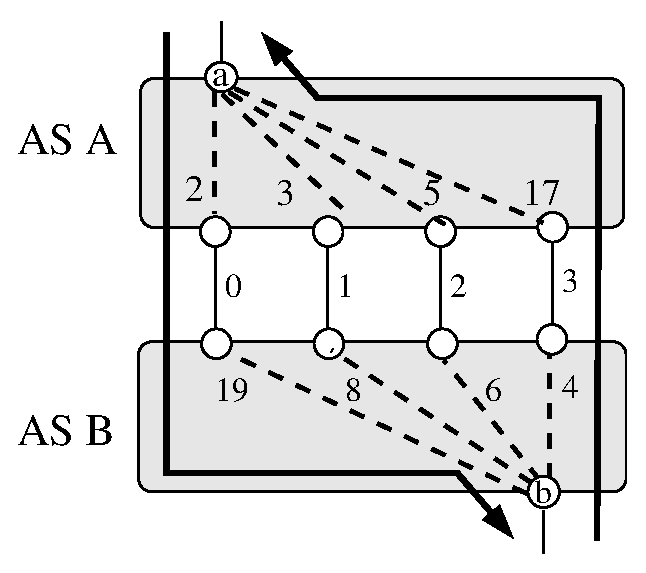
\epsfig{file=figures/hotpotato.eps, width=\linewidth}
\caption[How the IGP implements ``hot potato'' routing]{If router $I$ learns two or more routes that are equally good
up through Step~5 in Table~\ref{tab:background:decision}, it will select the route
whose next hop has a shortest IGP path cost.  IGP path costs are shown as
numbered edges; these path costs often correspond to geographic distance.}
\label{fig:background:hotpotato}
\end{minipage}
\end{figure}

%\begin{figure}
%\end{figure}


If multiple routes remain after Step~4, a router will prefer a route
that it learned via eBGP over one that it learned via iBGP.  If multiple
routes still remain, the router will prefer the route whose next-hop IP
address is ``closest'' in the internal routing topology (\ie, the
shortest IGP path).  This step allows a network to achieve what is
commonly referred to today as ``hot potato routing'': the process by
which an AS tries to offload traffic to neighboring ASes as quickly as
possible.\footnote{``Hot potato routing'' was initially coined by Paul
Baran for {\em all} routing techniques where nodes would forward
messages as quickly as possible~\cite{hafner1996}.  This notion stood in
contrast to quintessential ``store and forward'' networks like the
telegraph.  In these systems, the electrical signal would dissipate
after some distance.  As such, relay nodes would transcribe the message
in Morse code, and an operator would then re-feed the ticker to
the relay node, which would regenerate the electrical signal.}  
Figure~\ref{fig:background:hotpotato} illustrates this mechanism.  A network
operator could conceivably control interdomain traffic by adjusting edge
weights in the IGP. Unfortunately, updates in the IGP topology
can cause unexpected and unwanted shifts in BGP routes, potentially
affecting large volumes of traffic~\cite{teixeira2004b}.

If multiple routes remain after the IGP tiebreak, the routers may break
ties in a number of ways.  This final tiebreak is usually based on the
``router ID'' of the router that advertised the route, although other
tiebreaking mechanisms are sometimes used, such as selecting the ``most
stable'' route (\ie, the one that has been advertised for the longest
period of time).

A key problem operators face is determining which route each router in
the AS will select.  It might seem that this process might be as simple
as taking the set of eBGP-learned routes for a destination and applying
the process in Table~\ref{tab:background:decision} at each router.  In
fact, predicting the outcome of this process is not so simple:
Chapter~\ref{chap:sandbox} is 
dedicated to solving this problem.


\subsection{Putting It Together: How Traffic Gets from Here to There}

We now describe how IGP, iBGP, and eBGP act in
concert to establish routes between various endpoints.  One can think of
a route in terms of two distinct phases: (1)~the route to some exit (or
``egress'') router in that AS (or to the ultimate destination, if the
destination is located in the same AS) and (2)~the route from the egress
point to the appropriate next-hop AS.

%\subsubsection{Routing Within a Single AS: Internal BGP (iBGP) and IGP}

An example of the route to a destination in a router's routing table is
shown in Figure~\ref{fig:bgpex}: each destination prefix has a next-hop
IP address to which to send traffic.  If the destination is in a different
AS and the router is not an egress router, then that next hop is
typically the IP address of an egress router.  The BGP route selection
process determines which egress router each router sends
traffic to: each router in the AS may learn a route for some destination
from one or more egress routers, but ultimately selects only one of
those routes.  The AS's IGP is then responsible for determining the
route from that router to the egress router named by that next-hop IP
address.

If, on the other hand, the destination is in a remote AS and the router
is an egress router, the router will either select a route with a next
hop that is in a neighboring AS, or it will select a route learned from
a different egress router and rely on the AS's IGP to forward traffic to
the egress router with that next-hop IP address.


%%%%%%%%%%%%%%%%%%%%%%%%%%%%%%%%%%%%%%%%%%%%%%%%%%%%%%%%%%%%

\section{Internet Routing Configuration}\label{sec:conf}

Internet routing's true complexity
lies in the fact that so many aspects of the routing protocol's
operation are manipulable with configuration.  
As discussed in Chapter~\ref{chap:intro}
(Section~\ref{sec:intro:config}), and as we will see throughout this
dissertation, many of the problems faced by the Internet routing system result
from the protocol's configurability.


This section provides background on Internet routing configuration.
Internet routing configuration languages typically have thousands of
distinct commands~\cite{www-cisco-ios-master}; the reader will be
pleased to learn that we will not survey all of them here.  Rather, we
first classify the {\em semantics} of routing configuration into three
main operations: ranking, filtering, and dissemination.  We then provide
a brief example of Cisco router configuration {\em syntax} to
demonstrate how a network operator can implement these
operations in practice.

\subsection{Semantics: Ranking, Filtering, Dissemination}
\label{sec:semantics}

\begin{figure}
%\centering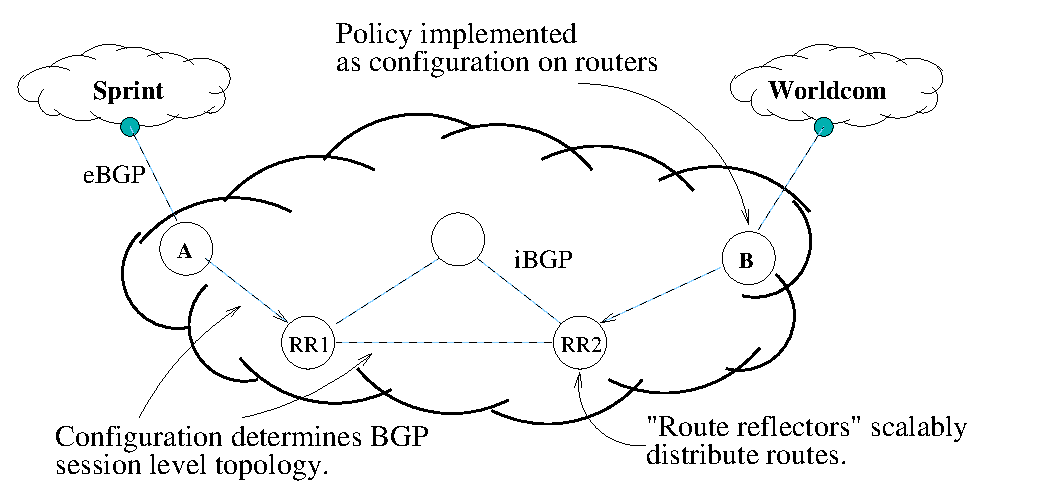
\epsfig{file=rcc/figures/overview.eps, width=\linewidth}
\centering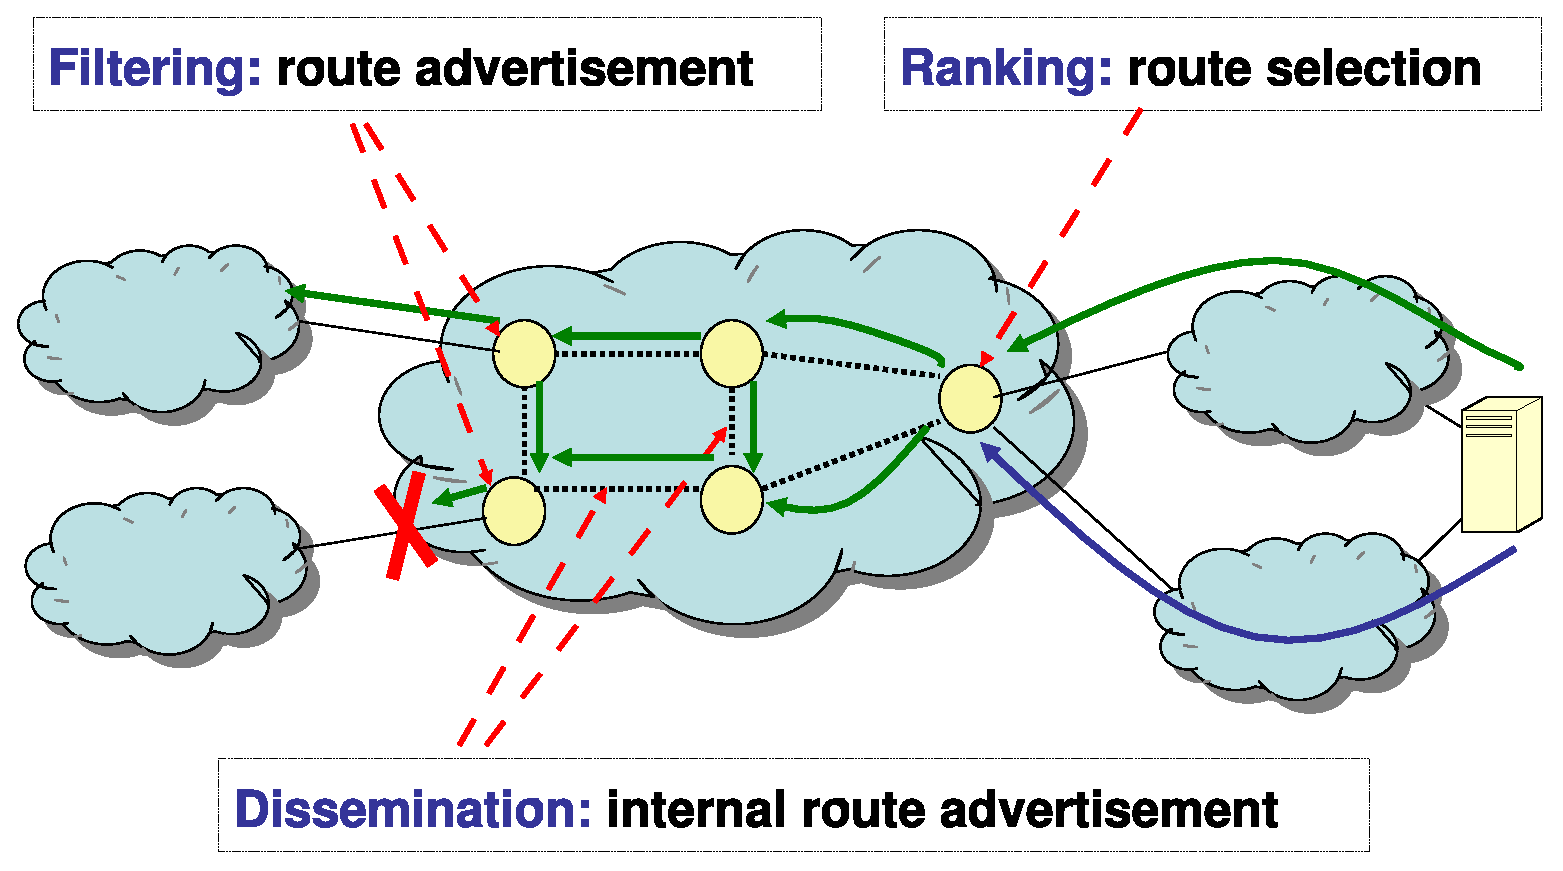
\epsfig{file=rcc/figures/factoring2.eps, width=\linewidth}
\caption{BGP configuration semantics.}
\label{fig:overview}
\end{figure}

Internet routing configuration allows the routing protocol to achieve
two important goals:
\begin{enumerate}
\itemsep=-1pt
\item {\em Policy.}  
Internet routing must be flexible enough to implement complex business
relationships.  Internet routing configuration provides network
operators the ability to encode these policies in router configurations.
\item {\em Scalability.} The Internet must scale to a large number of
hosts, routers, and ASes.  To achieve this scalability, Internet
routing configuration allows an operator to specify various ways for the
routing protocol to aggressively aggregate routing information (\eg,
using route reflection).
\end{enumerate}

The rest of this section describes how routing configuration's three
main operations---ranking, filtering, and dissemination---facilitate
the expression of complex business policies and provide options for
achieving scalability.  We also briefly explain how each of these
operations can affect the correctness and predictability of Internet
routing. 

\subsubsection{Policy: Ranking and Filtering}

The bilateral business relationships established between ASes (as
described in Section~\ref{sec:structure}) imply that the {\em policy}
afforded by Internet routing configuration should provide a network operator
two degrees of control: (1)~which route each router in the AS should
prefer, given multiple routes to a destination ({\em ranking});
(2)~which routes should be advertised to which neighboring ASes ({\em
filtering}).  Table~\ref{tab:business} summarizes these common practices
for both ranking and filtering.  Although these practices constitute the
conventional wisdom for how ASes operate, Section~\ref{sec:bg_stability}
presents examples of some common deviations from these practices.  We
now explain these practices in more detail in this section.

\begin{table}
\centering\begin{tabular}{p{1in}||p{2.35in}|p{2.05in}}
\parbox{1in}{{\em Type of \\neighboring AS}}  & {\bf Ranking} & {\bf
Filtering} \\ \hline  
{\bf Customer} & Most preferred & 
Advertise to all other ASes \\ 
{\bf Peer} & Less preferred than routes through customer, more preferred
than routes through provider & Advertise to customer ASes \\
{\bf Provider} & Least preferred & Advertise to customer ASes
\\
\end{tabular}
\caption[Common business relationships and practices between
ASes]{Common business relationships and practices between ASes on the 
Internet today.  Although this table summarizes the conventional wisdom
of how ASes commonly interact today, Section~\ref{sec:bg_stability}
describes several violations of these practices.}
\label{tab:business}
\end{table}

Because a customer pays a provider per unit traffic regardless of the
direction the traffic is flowing, it is to an AS's advantage to select
routes to destinations via its customer ASes, given the option.
Similarly, an AS would typically prefer to send traffic through one of
its peers (which it can do at no additional cost) versus sending traffic
via one of its providers (which will charge it for the service of
carrying that traffic).


A router's configuration can prevent a certain route from being accepted
on inbound or readvertised on outbound.  Configuring filtering is
complicated because global behavior depends on the configuration of
individual routers. An AS will
typically advertise its entire set of routes to its customers (who it
will gladly charge to carry traffic to any of those destinations) but
will only advertise to one of its peers the routes that it learned from
one of its customers.  On the other hand, an AS will not advertise
routes that it learns from one if its providers to another one of its
providers: doing so would cause that AS to provide transit between two
of its providers and pay {\em both} of its providers to boot!


\subsubsection{Scalability: Dissemination}\label{sec:dissemination}


\begin{figure}
\centering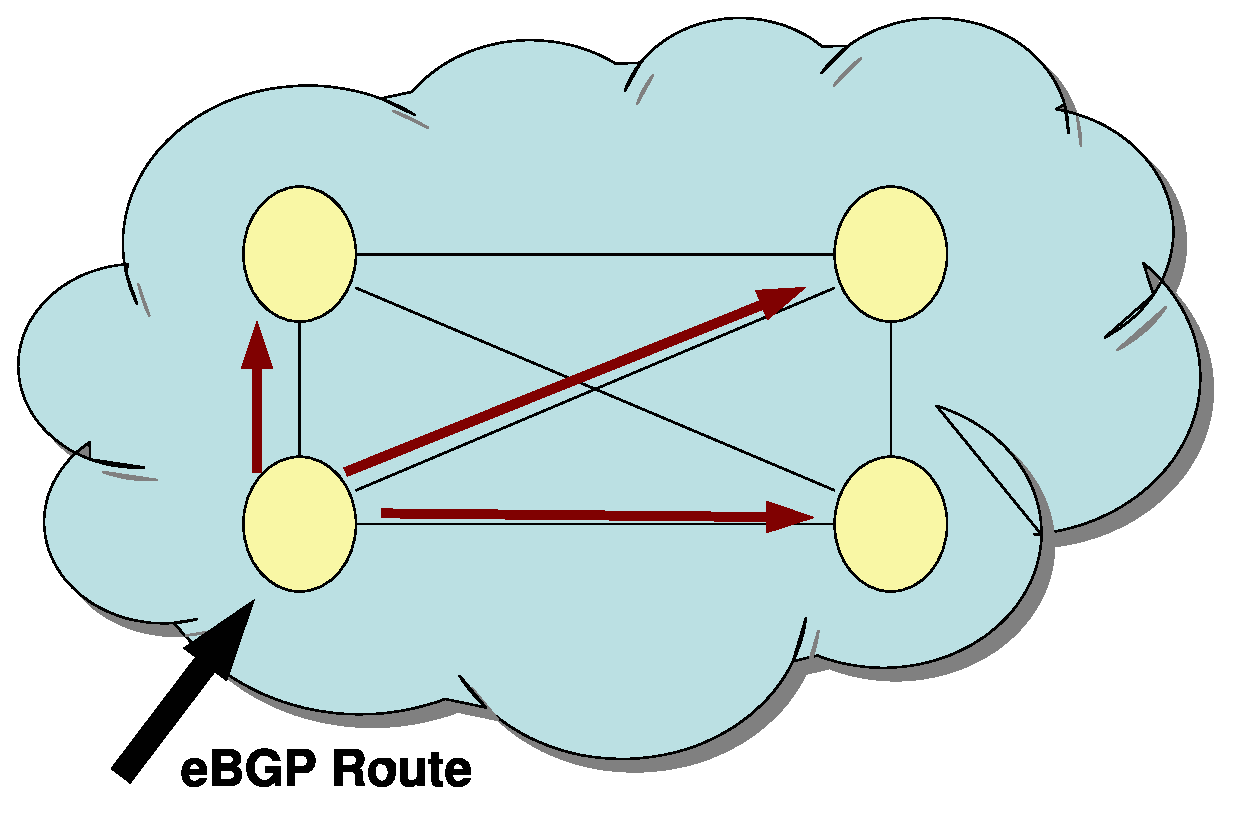
\epsfig{file=figures/fullmesh.eps, width=0.4\linewidth}
\caption[Internal BGP configuration for small ASes: ``full mesh''
topology]{Small ASes establish 
a clique (or ``full mesh'') of iBGP 
sessions.  Each circle represents a router within an AS.  Only
eBGP-learned routes are readvertised over iBGP sessions.}
\label{fig:fullmesh}
\end{figure}

\begin{figure}
\centering
\subfigure[Routes learned from clients are readvertised over all iBGP
sessions.]{
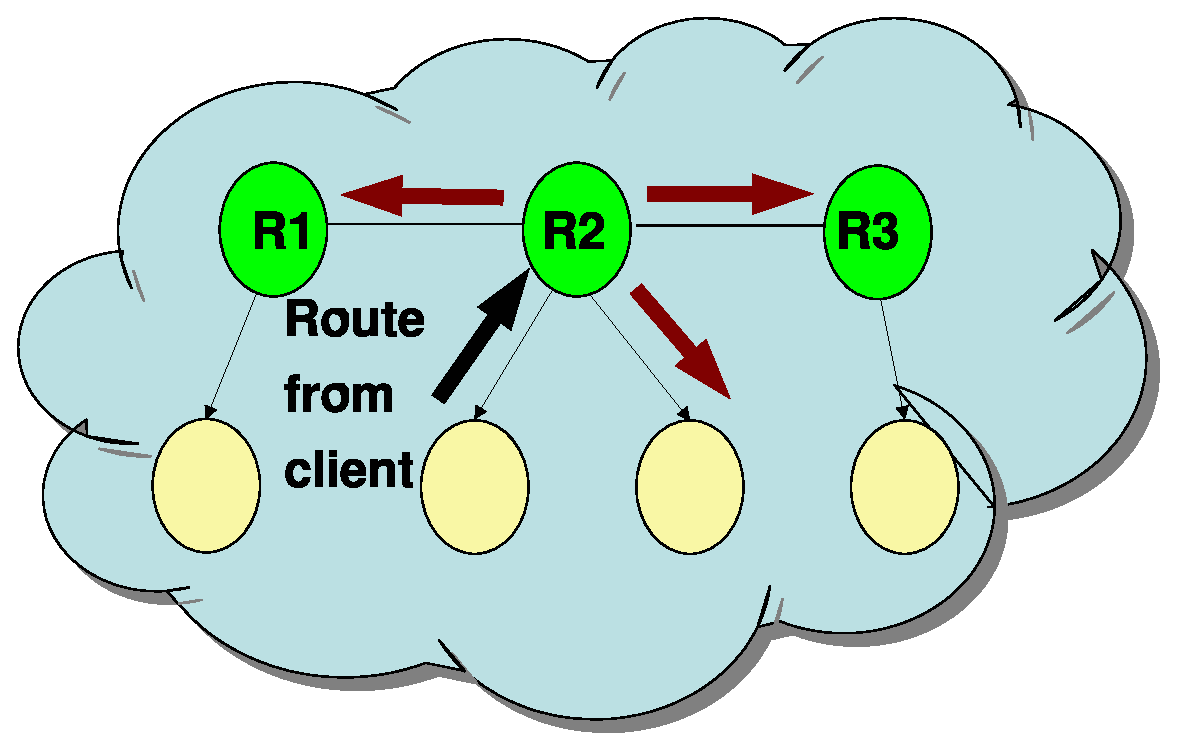
\epsfig{file=figures/rr1.eps, width=0.45\linewidth}}\hfill
\subfigure[Routes learned from non-clients are readvertised to clients only.]{ 
\epsfig{file=figures/rr2.eps, width=0.45\linewidth}}
\caption[Internal BGP configuration for large ASes: route reflector
topology]{Larger ASes commonly use route reflectors, which advertise
some iBGP-learned routes as described above. Directed edges between routers
represent iBGP sessions from route reflectors to clients (\eg, router
$R2$ is a route reflector with two clients). As in
Figure~\ref{fig:fullmesh}, all routers readvertise eBGP-learned routes
over all iBGP sessions.}
\label{fig:ibgp_rr}
\end{figure}

A router's configuration controls the {\em dissemination} of routes
within the AS and between neighboring ASes by allowing each router to 
establish BGP sessions with neighboring routers.  Router configuration
allows an the router to establish two types of BGP sessions: those to
routers in its own AS (iBGP) and those to routers
in other ASes (eBGP).  A small AS with only two or
three routers may have only 10 or 20 BGP sessions, but large backbone
networks may have more than 10,000 BGP sessions, more than half of
which are iBGP sessions.  

BGP messages propagate differently depending on whether the update
is propagating over an eBGP session or an iBGP session.  An eBGP session
is typically a {\em point-to-point} session: that is, the IP addresses
of the routers on either end of the session are directly connected with
one another and are typically on the same local area network.  There
are, of course, exceptions to this practice (\ie, ``multi-hop
eBGP''~\cite{www-ebgp-multihop}), but directly connected eBGP sessions
is normal operating procedure.  In the case where an eBGP session is
point-to-point, the next-hop attribute for the BGP route is guaranteed
to be reachable, as is the other end of the point-to-point connection.
A router will advertise a route over an eBGP session regardless of
whether that route was originally learned via eBGP or iBGP.

On the other hand, an iBGP session may exist between two routers that
are {\em not} directly connected, and it may be the case that the
next-hop IP address for a route learned via iBGP is more than one
IP-level hop away.  In fact, as the next-hop IP address of the route is
typically one of the border routers for the AS, this next hop may not
even correspond to the router on the other end of the iBGP session, but
may be several {\em iBGP} hops away.  In iBGP, the routers thus rely on
the AS's internal routing protocol (\ie, its IGP) to both (1)~establish
connectivity between the two endpoints of the BGP session and
(2)~establish the route to the next-hop IP address named in the route
attribute.  

The session-level iBGP topology determines how BGP routes propagate
through the network.  By default, a router will only readvertise a route
on an iBGP session if it learned that route via an eBGP session.  This
constraint requires that every router in an AS have an iBGP session with
every router that learns routes via eBGP (typically every other router),
as shown in Figure~\ref{fig:fullmesh}; \ie, those routers must form a
clique (the networking community commonly refers to this configuration
as a ``full mesh'' iBGP topology).

ASes with a small number of routers are often configured in a full mesh
iBGP topology, but a fully meshed iBGP topology requires $O(n^2)$
sessions for an AS with $n$ eBGP-speaking routers, which does not scale
well.  Two alternatives have been proposed to solve these problems:
route reflection~\cite{rfc2796} and confederations~\cite{rfc3065}.  To
improve scalability, larger networks typically use {\em route
reflectors}.  A route reflector selects a single best route and
announces that route to all of its ``clients''.  A route reflector is
defined by the fact that it has {\em client} routers, and it
readvertises its iBGP-learned routes to some other routers in the same
AS according to the following rules: (1)~if a route reflector learns a
route via eBGP or via iBGP from one of its clients, it readvertises that
route over all of its sessions to its clients; (2)~if it learns the
route via iBGP from a router that is not one of its clients, it
readvertises the route to its client routers {\em but not over any other
iBGP sessions}.  Figure~\ref{fig:ibgp_rr} shows an example route
reflector hierarchy and how routes propagate from various iBGP sessions.

Configuring an iBGP topology correctly is relatively difficult; we
discuss iBGP misconfiguration in more detail in
Section~\ref{sec:visibility}.  Incorrect iBGP topology configuration can
create many types of incorrect behavior, including persistent forwarding
loops and oscillations~\cite{Griffin2002}.
%Route reflection creates problems both for correctness and for modeling.
Route reflection causes problems with correctness because not all route
reflector topologies are guaranteed to propagate a route learned via an
eBGP session (\ie, not all iBGP topologies satisfy path visibility).  We
describe this problem in more detail in Chapter~\ref{chap:rcc}.  

Route reflectors also complicate predictability because they prevent each
router from learning every BGP route.  Thus, the BGP route that each
router ultimately selects may not be the same route that it would have
selected had it learned every BGP route for that destination (as it
would have in a full mesh iBGP topology).  This property makes route
prediction 
more difficult because the routes that some routers ultimately select
depend on the routes that other routers in the AS select.  Efficiently
computing the route that each router selects thus requires determining
these dependencies and ``visiting'' the routers within the AS in the
correct order.  Chapter~\ref{chap:sandbox} describes in more detail how
route reflection complicates predicting route selection within an AS.

Dissemination primarily concerns flexibility in iBGP configuration, but
the configuration may also {\em manipulate} route attributes when
disseminating routes for one of the following reasons: (1)~controlling
how a router ranks candidate routes, (2)~controlling the ``next hop'' IP
address for the advertised route, and (3)~``tagging'' a route to control
how the ranking and filtering functions on other routers treat it.


\subsection{Syntax: Routing Configuration Languages}\label{sec:configuration}

\begin{figure}
{\tt
        router bgp 7018\\
          \hspace*{0.2in} neighbor 192.0.2.10 remote-as 65000\\
          \hspace*{0.2in} neighbor 192.0.2.10 route-map IMPORT in\\ \\
          \hspace*{0.2in} neighbor 192.0.2.20 remote-as 7018\\
          \hspace*{0.2in} neighbor 192.0.2.20 route-reflector-client\\
        !\\
        route-map IMPORT permit 1\\
          \hspace*{0.2in} match ip address 199\\
          \hspace*{0.2in} set local-preference 80\\
        !\\
        route-map IMPORT permit 2\\
          \hspace*{0.2in} match as-path 99\\
          \hspace*{0.2in} set local-preference 110\\
        !\\
        route-map IMPORT permit 3\\
          \hspace*{0.2in} set community 7018:1000\\
        !\\
        ip as-path access-list 99 permit \^{}65000\$ \\
        access-list 199 permit ip host 192.0.2.0 host 255.255.255.0\\
        access-list 199 permit ip host 10.0.0.0 host 255.0.0.0
}
%% $ (make emacs happy)
\caption{Example of a Cisco router configuration.}
\label{fig:cisco_config}
\end{figure}

Figure~\ref{fig:cisco_config} shows an example of how ranking,
filtering, and dissemination are
encoded into a router configuration for a single router. The example
shows an excerpt from a Cisco router configuration; each router vendor
has a different configuration language, although many are similar to
Cisco's.  The first clause indicates that this router is located in
AS~7018.  BGP sessions to neighboring routers are indicated with the
{\tt neighbor} statements.  The router has a BGP session with IP address
{\tt 192.0.2.10} in AS~65000.  

The second {\tt neighbor} statement specifies that the ``inbound route
map'' (\ie, import policy) called {\tt IMPORT} should be applied to the
route advertisements learned on this BGP session.  This policy has two
clauses that implement the import policy.  The first clause assigns a
local preference value of 80 for advertised routes to {\tt 192.0.2.0/24}
and {\tt 10.0.0.0/8}, as defined in access-list 199.  The second clause
assigns a local preference of 110 to routes with an AS path of 65000
(\ie, a one-hop path to AS 65000).  All remaining routes are assigned
the default local preference value, 100, and tagged with a ``community''
value of {\tt 7018:1000}.  By itself, the community value has no
meaning; it is nothing more than a label.  Some other router's
configuration, however, may have an import or export policy that takes
some action (\eg, filtering the route, changing its local preference
value, etc.) based on this value.  Setting the community attribute on
one route and acting on that community on another introduces
dependencies across routers that can be difficult to debug.

This router also has a BGP session to a router with the IP address
{\tt 192.168.2.20}. The {\tt remote-as} command indicates that this
router is in AS 7018---the same as the router of this AS, as specified with
the {\tt router bgp} statement---which implicitly configures this
session as an iBGP session.  The next line of the configuration
indicates that {\tt 192.168.2.20} is a route reflector client.  No
additional configuration (beyond simply setting up a regular iBGP
session) is required on the client router to establish that it is a
client.

Figure~\ref{fig:cisco_config} shows an excerpt of a Cisco configuration,
but a noteworthy aspect of BGP configuration is that {\em the
configuration language is not standardized}.  As a result, an AS may
contain routers from many different vendors (\eg, Cisco, Juniper, Avici,
etc.).  Although all routers can exchange routes using the standard
BGP message format, their configuration languages are often different.
This heterogeneity makes the static configuration analysis problems
described in Chapters~\ref{chap:rcc} and~\ref{chap:sandbox} even more
challenging.

%%%%%%%%%%%%%%%%%%%%%%%%%%%%%%%%%%%%%%%%%%%%%%%%%%%%%%%%%%%%

\section{Related Work}\label{sec:rw_challenges}


While Internet routing achieves its policy and scalability goals fairly
well, the high 
degree of configurability that allows these goals to be met also
presents challenges both for {\em correctness} (\ie, preventing mistakes
and unintended interactions) and for {\em predictability} (\ie,
determining offline how the protocol will behave in practice).  This
section surveys previous approaches to addressing these two challenges
and how they relate to the work in this dissertation.

\subsection{Correctness}
\label{sec:rcc_related}

Operator-induced configuration faults are perhaps the single biggest
threat to the correct operation of Internet routing today.
%Both IDC and the Gartner Group estimate that between 70 to 80 percent of
%all routing problems resulting in network downtime are caused by network
%operators making changes to the network configuration; most of those
%changes are accidental or unintentional.  
After surveying previous
studies on the effects of configuration faults (and resulting
routing instability) on end-to-end performance, we survey previous work
on configuration management tools, which help operators audit
configuration changes and detect faults.

\subsubsection{How Routing Problems Affect Connectivity and Performance
(Why Correctness Matters)} 

\begin{center}
\begin{table}[ht!]
\begin{tabular}{l|l|l|p{2in}} 
{\bf Year} & {\bf Author} & {\bf Analysis Technique} & {\bf Major
Results} \\ \hline
\multicolumn{4}{c}{{\em How Configuration Faults Affect End-to-End
Performance}} \\ \hline 
2002 & Mahajan \ea~\cite{Mahajan2002} & Measurement/Email survey & 30\%
of all configuration ``slips'' that cause short-lived BGP announcements
disrupt connectivity. \\
2002 & Griffin \ea~\cite{Griffin2002} & Theoretical analysis & Some iBGP
configurations can cause protocol oscillations and persistent forwarding
loops.\\ \hline 
%
\multicolumn{4}{c}{{\em How Routing Instability Affects End-to-End
Performance}} 
\\ \hline 
1997 & Paxson~\cite{Paxson97} & End-to-end measurement & Routing-induced
path failures for 0.21-0.5\% of end-to-end observations.   \\
2001 & Labovitz \ea~\cite{labovitz:ton01} & Fault
injection & Up to 30\% packet loss during periods of routing instability\\ 
2003 & Feamster \ea~\cite{Feamster2003} & End-to-end measurement & 50\%
of all end-to-end path failures correlate with BGP instability. \\
2005 & Bush \ea~\cite{Bush2005} & Fault injection  & 85\% of BGP instability
events cause loss periods of 15 seconds or longer. \\
%
\hline\multicolumn{4}{c}{{\em How Protocol Artifacts Affect End-to-End
Performance}} \\ \hline 
2001 & Labovitz \ea~\cite{labovitz:ton01} & Measurement/Analysis & Some
failures take up to 15 minutes to converge after failover.  Some routers
may explore $O(n!)$ paths, where $n$ is maximum AS path length.\\
2001 & Griffin \ea~\cite{Griffin2001} & Simulation & Advertisement timer
settings significantly affect convergence time.\\
2002 & Mao \ea~\cite{Mao2002} & Simulation & Route flap damping can slow
convergence by several orders of magnitude. \\
\end{tabular}
\caption{The results of previous empirical studies of the effects of
routing faults and protocol artifacts on routing convergence or
end-to-end performance.} 
\label{tab:empirical_results}
\end{table}
\end{center}




Many researchers have studied both the effects of misconfiguration and
routing instability on network downtime and end-to-end performance.  This
section highlights the results of some previous studies, which provide
supporting evidence for the adverse effects of routing instability on
end-to-end performance.
%
Table~\ref{tab:empirical_results} summarizes these previous findings in
terms of three categories: those that study the effects of configuration
faults on end-to-end performance, those that study the effects of routing
instability on end-to-end performance, and those that study the effects of
various routing protocol artifacts on routing stability and convergence
(both of which indirectly affect end-to-end performance).  

Mahajan \ea studied the effects of BGP misconfiguration on connectivity
disruptions~\cite{Mahajan2002}.  This work studied short-lived BGP
misconfiguration by analyzing transient, globally visible BGP
announcements from an edge network.  They defined a ``misconfiguration''
as a transient BGP announcement that was followed by a withdrawal within
a small amount of time (suggesting that the operator observed and fixed
the problem).  They found that many misconfigurations are caused by
faulty route origination and incorrect filtering.
\rcc (Chapter~\ref{chap:rcc}) can help operators find these faults; it can also
detect faults that are difficult to quickly locate and correct.  \rcc
also helps operators detect the types of misconfigurations found by
Mahajan {\em et al.}~\cite{Mahajan2002} {\em before} deployment.

Griffin \ea examine two aspects of {\em iBGP} correctness that may
affect the end-to-end delivery of traffic: non-convergence and
``deflections'', whereby packets do not follow their intended
path~\cite{Griffin2002}.  This work does not observe how often incorrect
iBGP routing occurs in practice.
%This work astutely observes that the
%conditions for convergence under iBGP with route reflection are
%analogous to those specified by Gao and Rexford for eBGP.

Previous work has gathered evidence to suggest that routing
instability and configuration faults have serious
ramifications for end-to-end connectivity.
Paxson studied the end-to-end properties of Internet paths by performing
two separate experiments between $37$ hosts distributed
across the Internet; each path was probed with {\tt traceroute}
approximately once every day or two (in a second experiment, a fraction
of the paths were probed approximately once every two
hours)~\cite{Paxson97}.  Each experiment was conducted over the course
of approximately 6 weeks. The first experiment was in 1994, and the
second was in 1995.  In this work, Paxson studied both general routing
pathologies (\eg, asymmetric paths, erroneous routing, route flapping),
and also studied the times during which paths were 
unreachable due to failures of the routing infrastructure.  Paxson found
that paths were unavailable for 0.21\% of the time 
in his first sample and 0.5\% of the time during his second experiment.

In 2002-2003, Feamster \ea performed a similar study on the RON
testbed~\cite{Andersen-ccr2003} over the course of 13 months.  This work
extended Paxson's study by incorporating both more frequent active
probes (each of approximately 900 geographically and topologically
diverse paths was probed at least once every 90 seconds), which
triggered {\tt traceroute} probes upon detecting a reachability failure.
The BGP routing information was collected at sites that were co-located
with the measurement hosts~\cite{Feamster2003}.  About half of the
end-to-end failures observed coincided with some BGP routing
instability.  This study considered only correlation between BGP routing
instability with end-to-end path failures; an interesting future
direction would be to determine how many of the path failures were {\em
caused} by routing instability (\ie, cases where the routing protocol
actually disrupted communication) versus those that were simply
reflected by instability.





Labovitz \ea observed that BGP undergoes a process called ``path
exploration'', a process by which routers select (and propagate)
alternate routes upon learning a route withdrawal~\cite{labovitz:ton01}.
They showed that, in theory, during convergence, a router may explore
$O(n!)$ alternate 
routes, where $n$ is the maximum AS path length to the destination.  To
study this phenomenon in practice, they injected routing faults into the
running network and measured the duration of the convergence process,
finding that convergence may take as long as 15 minutes when a route is
withdrawn~\cite{labovitz:ton01}.  Bush \ea performed a similar study
that artificially injected routing updates into the network from ``BGP
beacons''~\cite{Mao2003b}; this experiment created instability on a
small set of paths, on which they then perform more targeted
observations to study the properties of end-to-end paths during these
periods of instability.  While they observe that many periods of
prolonged loss do not correlate with routing instability, they also find
that most episodes of routing instability cause periods of prolonged
loss.

Several other researchers have examined the effects of various protocol
artifacts on convergence time.  Mao \ea observed that damping routes
that oscillate can cause significant delays in convergence; in
pathological topologies, BGP may take roughly an hour to converge after
a single route withdrawal~\cite{Mao2002}.  Other work has simulated the
effects of BGP's timer settings on convergence time~\cite{Griffin2001}.
This dissertation does not address correctness problems that occur
during the convergence process.

%Our work focuses on {\em whether BGP will operate correctly
%at all}, regardless of timing and faults.



%\subsubsection{Fault Detection in Other Settings}



%%%%%%%%%%%%%%%%%%%%%%%%%%%%%%%%%%%%%%%%%%%%%%%%%%%%%%%%%%%%
%%%%%%%%%%%%%%%%%%%%%%%%%%%%%%%%%%%%%%%%%%%%%%%%%%%%%%%%%%%%
%%%%%%%%%%%%%%%%%%%%%%%%%%%%%%%%%%%%%%%%%%%%%%%%%%%%%%%%%%%%


\subsubsection{Configuration Management Tools: Helping Operators Cope
with Complexity}

\begin{table}
\begin{footnotesize}
\begin{tabular}{l|p{0.35in}|p{0.5in}|p{0.5in}|p{0.6in}|p{0.5in}|p{0.5in}|p{0.5in}}
& {\bf Traffic eng.} & {\bf Failure Analysis} & {\bf Static Fault Detection} & {\bf Monitoring} &
{\bf Inventory} & {\bf Revision Mgmt.} & {\bf ``Automated'' Configuration} \\ \hline
\multicolumn{8}{c}{{\em Fault Detection and Traffic Engineering}} \\ \hline
NetSys/IPAT~\cite{www-wandl-ipat} & & $\B$ & $\B$ &  & & & $\B$ \\
OpNet SP Guru~\cite{www-opnet-spguru} & & $\B$ &  & & & & \\ 
Cariden MATE~\cite{www-cariden-mate} & $\B$ & & & & & \\ 
\hline
\multicolumn{8}{c}{{\em Change Management}} \\ \hline
%rancid & & & & & & $\B$ & \\
Intelliden R-Series~\cite{www-intelliden} &  & & & & $\B$ & $\B$ & \\
Redcell~\cite{www-redcell} &  & & & & & $\B$ & \\
VoyenceControl~\cite{www-voyencecontrol} &  & & & & & $\B$ & \\
Opsware NAS~\cite{www-opsware} &  & & & & & $\B$ & \\
Tripwire~\cite{www-tripwire} &  & & & & & $\B$ & \\ \hline
%TrueControl~\cite{www-truecontrol} & & & & & & $\B$ & \\ \hline
\multicolumn{8}{c}{{\em Route Analytics}} \\ \hline
HP RAMS~\cite{www-hp-rams} & & & & $\B$ & & & \\
RouteDynamics~\cite{www-ipsumnetworks} &  & & & $\B$ & & & \\
Route Explorer~\cite{www-packetdesign} & & & & $\B$ & & & \\
\end{tabular}
\end{footnotesize}
\caption[Existing configuration management tools]{Existing configuration
management tools, which 
generally fall into three categories: fault detection and traffic
engineering, change management, and route analytics.  The fault
detection tools are most related to \rccns, and the traffic engineering
tools are most related to the model and tool in
Chapter~\ref{chap:sandbox}.  Change management tools 
help an operator audit configuration changes and revert to a previous
version of the configuration when faults are discovered.  Route
analytics products rely on analyzing protocol {\em dynamics} to detect
faults.}
\label{tab:mgmt}
\end{table}


Many network operators use configuration management tools such as
``rancid''~\cite{www-rancid}, which periodically archive and manage
versions of router
configurations.  When a network problem
coincides with the configuration change that caused it, these tools can
help operators revert to an older configuration.  Unfortunately, a
configuration change may induce a fault
that becomes active later,
and these tools do not detect whether the configuration has these types
of faults in the first place.

Some tools analyze network configuration and highlight
rudimentary configuration errors.  One such tool was Cisco's
Netsys-Agent, which was decommissioned in November 2000 and evolved into
a product called IP Analysis Tools (IPAT), supported by the Wide Area
Network Design Laboratory~\cite{www-wandl-ipat}.  IPAT periodically
collects the configurations from the network's devices and helps
network operators diagnose ``connectivity issues''.  The product also
allows network operators to evaluate ``what-if'' scenarios (\ie, how a
particular configuration change will affect network connectivity and
topology), verify that a network configuration satisfies 
connectivity requirements (\eg, that two nodes in the network can reach
each other), and evaluate various failure scenarios.  IPAT also provides
graphical interfaces to network operators that assist them in viewing
router configurations and routing tables.
% http://www.wandl.com/html/ipat/IPAT_new.cfm

OpNet's NetDoctor product analyzes the configurations of many routing
protocols, including OSPF, IS-IS, RIP, MPLS, and
BGP~\cite{www-opnet-netdoctor}.  A white paper on NetDoctor provides
examples of the types of fault detection that the tool performs, such
as: checking that two interfaces on the opposite ends of an OSPF edge
are in the same area, checking consistency of BGP ``hold timer'' values,
checking for redundant access control lists, enabling system logging,
blocking ICMP and telnet, etc.~\cite{www-opnet-netdoctor-wp}
NetDoctor also appears to allow operators to check their
configurations against best common practice (an issue we also tackle in
Section~\ref{sec:validity}).  Although the checks performed by NetDoctor
are similar in spirit to those performed by \rcc
(Chapter~\ref{chap:rcc}), the work we present in this dissertation focuses
more on verifying {\em network-wide} properties of routing, rather than
simply performing checks on the consistency of the configuration of a
single router (or pair of routers)---NetDoctor does not implement these
types of checks.

Intelliden provides a product called R-Series, which helps network
operators keep track of device inventory and changes to the network
configuration~\cite{www-intelliden}. The product provides: (1)~a device
modeling application, which translates the differing configuration
languages for a device (\ie, depending on vendor, type, model, and
operating system) into a single, independent XML representation, (2)~a
system for managing version histories of the network configuration,
and (3)~a framework for managing device inventory.  Intelliden's R-Series
does not provide any automated fault detection or
debugging support; it is primarily a tool to help network operators
manage the complexity that results from heterogeneous devices and
multiple network operators who can make changes to the configuration.

Several other similar products exist to assist network operators with
auditing configuration changes: Redcell allows a network operator to
update the network configuration from a centralized location and also
performs version control and automated backup~\cite{www-redcell}.
Voyence's VoyenceControl allows an operator to configure network devices
from a centralized server and performs some validation of configuration
before deployment~\cite{www-voyencecontrol}.  Opsware's Network
Automation System~\cite{www-opsware}, and Tripwire~\cite{www-tripwire}
also monitor configuration changes to
network devices.

Other commercial tools do not directly analyze the configuration, but
rather monitor routing dynamics and network performance to assist
operators in finding problems (including possible configuration
faults).  Hewlett Packard (HP) offers a Route Analytics Management
System (RAMS)~\cite{www-hp-rams}, which 
participates in the routing protocol with the routers in the network,
actively detects problems related to OSPF, IS-IS, BGP, and EIGRP, and
reports these problems to the network operator.  RAMS also
correlates routing information with other performance data to help
network operators diagnose the underlying cause of a problem.
%% http://www.managementsoftware.hp.com/products/ovrams/twp/ovrams_twp_ip_route.pdf
HP's OpenView product line has many other tools designed to help
operators with network and application management~\cite{www-hp-openview}.
% http://www.openview.hp.com/products/a-z.html

Ipsum Networks (now defunct) developed a product called RouteDynamics
that actively participated in a network's 
IP routing protocols and monitored routing activity to predict and
analyze potential routing problems~\cite{www-ipsumnetworks}.  The
product primarily focuses on helping operators both detect routing
instability and identify the cause of the instability.  The product also
allows network operators to view and ``play back'' historical routing
data, as many of the routing instabilities that affect network
performance are transient.

Most network management tools detect rudimentary errors and track
changes to the network configuration for auditing purposes, but they do
not help a network operator determine whether a network configuration
will actually achieve the intended behavior.  A deficiency in today's
router configuration languages is that there is no high-level language
with which a network operator can specify policies.  The lack of such a
language not only makes configuring the network more complex,
but it also makes deducing faults more difficult: any fault detection
technique must infer the operator's intent solely from the low-level
configuration.  Recent work proposes a ``service grammar'' for BGP,
which includes a requirements language with which operators can specify
higher-level requirements against which the system can be
checked~\cite{Qie2003}.  While developing such a grammar
would ease the task of both specifying and validating routing
configuration, the proposed grammar is still rather low-level: for
example, it requires operators to specify requirements such as the
existence of a BGP session between pairs of routers, which routers are
route reflectors for which other routers, etc.  Such a grammar could
have just as many errors as the configuration itself and still does not
specify the intended behavior of the network at a high enough level
(\eg, load balance, backup links, etc.).

\subsubsection{Model Checking and ``Automated'' Configuration} 

Model checking has been successful in verifying the correctness of
programs~\cite{Godefroid97} and other network
protocols~\cite{Bargavan2002,Hajek78,Musuvathi2004}.  Unfortunately,
model checking is not ideal for verifying all aspects of BGP
configuration because it depends heavily on exhausting the state-space
within an appropriately defined environment~\cite{Musuvathi2003}.  The
behavior of an AS's BGP configuration depends on routes that arrive from
other ASes, some of which, such as backup paths, cannot be known in
advance~\cite{Feamster2003f}.  On the other hand, model checkers may
ultimately be appropriate for {\em generating} BGP configuration: Recent
work has proposed using a model checker to specify the parameters of a
high-level routing policy for a virtual private network and running
these parameters through a model checker~\cite{Narain2004}.  The output
of the model checker---a solution that satisfies all of the specified
constraints---are the configuration fragments themselves.  It is
conceivable that such an approach could be used to generate BGP
configuration as well.

A trend called ``automated configuration'' refers to techniques that
allow a network operator 
to configure the network using templates and graphical interfaces,
rather than by typing configuration commands on individual devices.
Another goal of these automated configuration projects is to assist
network operators in handling device heterogeneity by providing a
standard interface through which all devices in the network can be
configured.  

Recent work has proposed automation tools that build an inventory of
both intradomain routing and session-level interdomain routing
configuration~\cite{Feldmann2001} and automate enterprise network
configuration~\cite{Caldwell2003}.  These tools detect router and
session-level syntax errors only (\eg, undefined filters), a subset of
the faults that \rcc detects.  \rcc is the first tool to check {\em
network-wide properties} using a vendor-independent configuration
representation and the first tool that bases its tests on a high-level
specification of routing protocol correctness.

Automated configuration entails not only building an inventory of the
network-wide configuration, but also enabling an operator to configure
many heterogeneous network devices through a common interface.
Cisco is currently leading a research initiative in this
area~\cite{www-cisco-comer}. The IETF ``Netconf'' working group is also
actively developing a standard API over which network devices can be
managed via remote procedure calls; the group is also defining a
standard XML schema with which a network operator can send queries about
the network device~\cite{netconf-wg}.
More recent work has
proposed a technique for automating interdomain routing configuration
by representing the network configuration in a database, configuring the
network from the database itself, and automatically generating low-level
routing configuration from the specification in the
database~\cite{Feldmann2005}.  Some existing firewall and virtual
private network (VPN)
technologies, such as products from Reef Point~\cite{www-reefpoint},
also allow a network operator to configure network appliances from a
centralized database.  \rcc also normalizes the network-wide configuration
and stores it in a centralized database.  In this sense, it could be
seen as an element of a configuration automation system that
configures the network from a central location, checks
the configuration for errors, and subsequently pushes that configuration
to the actual devices distributed across the network.


% http://ftp.ietf.org/internet-drafts/draft-ietf-netconf-prot-06.txt
% http://www.csail.mit.edu/events/eventcalendar/calendar.php?show=event&id=375




\subsubsection{Correctness Problems that Span Multiple ASes}

The behavior of Internet routing depends on configuration that spans
many independently operated networks and administrative boundaries.
Internet routing configuration allows each AS to express policies
independently of every other AS.  Unfortunately, the policies of one AS
may interact with those of another in unexpected (and unintended) ways.
One serious undesirable consequence of this interaction is that the
protocol may oscillate---that is, it may continue to send cycles of
routing updates that do not reflect changes in the underlying
topology.  These oscillations (which we referred to as violations of
{\em safety} in Chapter~\ref{chap:intro}) can cause problems for both
performance and debugging.  Chapter~\ref{chap:policy} addresses how to
guarantee safety across multiple ASes; Section~\ref{sec:bg_stability}
discusses related work on this topic.

\subsection{Predictability}
\label{sec:te_related}



%In this paper, we presented an abstraction for router import policy;
%while similar to RPSL~\cite{rfc2622}, our abstractions are
%specifically designed to capture semantics that
%are relevant to protocol emulation.
%% Both of these projects rely on time-based
%% simulation of BGP, which is an unnecessarily complex (and sometimes
%% unintentionally nondeterministic) approach to achieving the set of
%% predicted routes for an AS.


%%   1. BGP "sufficient conditions": for protocol convergence
%%   - more specifically-related BGP work like the two SIGCOMM'02
%%     papers (Tim's, and the Bell Labs ones), and Tim's MED ICNP
%%     paper, and the paper lixin and i wrote on BGP convergence
%%     (the algo for box #3 partially derives from this)

%%   3. configuration: RPSL
%%   - RPSL, in terms of trying to normalize/represent configuration
%%     of BGP-related stuff


%%   4. BGP TE: our CCR submission -- you could wax poetic a bit on how
%%     the CCR papers suggests ways to select tweaks to make to the
%%     what-if-a-tron

%Several previous theoretical results inspired its design of the route
%prediction algorithm we present in this paper.


Previous work presented an IGP emulator that helps network operators
optimize link weights for intradomain traffic
engineering~\cite{Feldmann2000}. 
Cariden's Multiprotocol Automation and Traffic Engineering (MATE)
framework parses IGP routing configuration, estimates traffic demands,
performs IGP simulation and metric optimization, and helps network
operators with capacity and changeover planning, in addition to everyday
traffic engineering tasks~\cite{www-cariden-mate}.
% http://www.cariden.com/products/marcom/mate_overview_0401.pdf
These tools incorporate traffic demand data to model how routing changes
will affect traffic flow, but they do not model changes to BGP routing
policies or the effects of iBGP on path selection.  There has also been
much focus on modeling BGP {\em
convergence}~\cite{Gao2001a,Griffin2002c,labovitz:ton01,Sobrinho2003}
but the work in Chapter~\ref{chap:sandbox} is the first to model BGP
{\em route selection\/}.

OpNet's SP Guru~\cite{www-opnet-spguru} helps network operators perform
traffic engineering and failure analysis within a single domain.  Such
tools have similar applications to the model of {\em interdomain}
routing that we present in Chapter~\ref{chap:sandbox}.  SP Guru can
model the network, given the routing configuration as input, to provide
a ``virtual network environment'', where a network operator can evaluate
potential changes to routing in the network.  One of the tool's stated
goals is to assist network operators in evaluating various types of
configuration changes before deploying a configuration on a live
network.  SP Guru also integrates with
NetDoctor~\cite{www-opnet-netdoctor}  (described earlier in this section).
% http://www.opnet.com/products/spguru/SPGuru_brochure.pdf

Network simulators (\eg, ns~\cite{www-ns-bgp}, C-BGP~\cite{www-cbgp},
SSFNet~\cite{www-ssfnet}) 
help operators understand dynamic routing protocol behavior, but
simulation represents network behavior in terms of message passing and
protocol dynamics over a certain period of time.  In contrast, network
engineers usually just need to know the outcome of the path-selection
process and not the low-level timing details.  Furthermore, existing
simulators do not capture some of the relevant protocol interactions
that can affect the outcome of the route selection process.  Simulating every
detailed interaction is difficult without a higher level model of BGP
in the first place.


Recent work proposes efficient techniques for large-scale parameter
optimization for various network protocols, including the tuning of the
local preference attribute in BGP~\cite{Ye2003}.  This work is
complementary to ours---the proposed search techniques could use the
routing sandbox (Chapter~\ref{chap:sandbox}) as the ``inner loop''.
These techniques currently use 
simulators such as C-BGP~\cite{www-cbgp} or SSFNet~\cite{www-ssfnet},
but the techniques only 
depend on the outcome of BGP path selection (not on dynamics) and would
likely benefit from having an efficient, accurate emulation tool as an inner
loop.  An accurate model of network-wide BGP route selection can also
improve the accuracy of simulators.  Recent 
work has built a system that takes the BGP and IGP
configurations from a single AS, as well as an estimate of traffic
demands, and searches for the appropriate configuration changes that
should be made to achieve a certain traffic engineering goal while
limiting the amount of ``churn'' (\ie, route changes)~\cite{Uhlig2004}.



The BGP model in Chapter~\ref{chap:sandbox} applies several previous
theoretical results in new ways.  The constraints for iBGP configuration
that we present in Section~\ref{sec:setup} are motivated by
previously derived sufficient conditions for iBGP to guarantee that the
routing protocols converge to a stable
assignment~\cite{Griffin2002b,Griffin2002}.  This work specified these
conditions to ensure correct routing behavior, but these constraints are
also required to {\em model} BGP routing.
%
The route prediction algorithm in Section~\ref{sec:fm_med} 
also uses results from previous work. We 
apply a constructive proof regarding stable inter-AS policy
configurations~\cite{Gao2001a} to iBGP configuration and used this proof
as the basis for predicting how a network with route reflectors will
select BGP routes.
%

In previous work, we explored practical traffic engineering techniques
in BGP; we had assumed the existence of a BGP emulator for testing traffic
engineering techniques offline~\cite{Feamster2003e};
Chapter~\ref{chap:sandbox} describes such a tool that uses algorithms
that {\em accurately} and {\em 
efficiently} predict the outcome of the BGP route selection process in
a single AS using only a snapshot of the network configuration and the
eBGP-learned routes from neighboring domains, without simulating
protocol dynamics~\cite{Feamster2004}.  The evaluation of this prototype
demonstrates that our algorithm is
accurate and efficient enough to be used in practice for many network
engineering tasks.  
%The work in Chapter~\ref{chap:sandbox} extends that
%work by: designing an 
%algorithm that models BGP path selection in networks that use {\em both}
%MEDs and route reflection; formally presenting the proofs, algorithms,
%and running time complexity
%for various cases of network configuration; formalizing the complexity
%introduced by MED and route reflection; and proposing protocol
%improvements that achieve the goals of MED and route reflection
%reduce modeling complexity, and prevent undesirable side effects (\eg,
%oscillations). 


%%%%%%%%%%%%%%%%%%%%%%%%%%%%%%%%%%%%%%%%%%%%%%%%%%%%%%%%%%%%
%%%%%%%%%%%%%%%%%%%%%%%%%%%%%%%%%%%%%%%%%%%%%%%%%%%%%%%%%%%%
%%%%%%%%%%%%%%%%%%%%%%%%%%%%%%%%%%%%%%%%%%%%%%%%%%%%%%%%%%%%



\section{Summary}

This chapter has provided the requisite background material on Internet
routing for reading the rest of this dissertation.  In the process of
introducing the basic operation of today's Internet routing protocol,
BGP, we have drawn attention to the aspects of the protocol that, though
they provide the necessary flexibility for network operations, introduce
a significant amount of complexity.  The rest of the dissertation
focuses on proactive techniques for providing correctness and
predictability guarantees in the face of this complexity.

Although this dissertation focuses on providing correctness and
predictability using static configuration analysis within the context of
{\em today's} routing protocol, the following chapters will draw out many
important lessons for designing future Internet routing protocols and
architectures.  Chapter~\ref{chap:concl} draws on some of these lessons
to propose a routing infrastructure called the Routing Control Platform
(RCP)~\cite{caesar2004,feamster:fdna2004}, whose ultimate goal is to
explicitly enforce 
various correctness guarantees.  
%We defer discussion of related
%proposals for routing protocols and architectures to
%Section~\ref{sec:rw_architectures}.

Network operators are often their own worst enemies concerning Internet
routing correctness and predictability, but malicious behavior also
poses a major threat to these goals.  This dissertation presents
techniques for protecting network operators from themselves, but our
next goal should be to protect it from adversaries.  This imminent
problem is not our focus (it is difficult enough to provide correctness
and predictability even when no parties are malicious!), but we discuss
some open problems in Internet routing security in the final chapter
(Section~\ref{sec:concl:security}).

We are now armed with a basic understanding of Internet routing and the
basic problems with guaranteeing correct and predictable behavior, but,
despite all previous work, our understanding of the properties that
constitute ``correct'' behavior are not sharp.  The next chapter
addresses this problem.


% I say Who's on first, What's on second, I Don't Know's on third.
%- Lou Costello 


\qchapter{\textit{One of the beautiful things about baseball is that every once in a while you come into a situation where you want to, and where you have to, reach down and prove something.}  
    \vskip 0.1em - Nolan Ryan}{Correctness Specifications for Internet
    Routing}\label{chap:rlogic}


%\chapter{A Logic for Internet Routing}\label{chap:rlogic}

%% \cs{T}he complexity of Internet routing configuration and protocol
%% dynamics mandates a framework for understanding and manipulating
%% Internet routing at a level of abstraction that facilitates reasoning
%% about whether or not the protocol is behaving ``correctly''.  Naturally,
%% the first step in this process is defining what it means for a routing
%% protocol to operate correctly in the first place.  Specifying
%% correctness is not easy, because it requires distilling a high-level
%% description of how the routing protocol should behave from the myriad
%% technical minutia of the operation of the protocol.

\cs{T}he flexibility offered by Internet routing configuration
allows the protocol to scale well and enables operators to express a wide
variety of policies, but it increases the complexity of the system.  This
complexity makes it difficult to reason about the behavior of Internet
routing, leading to {\em ad hoc} fixes to observed problems that
ultimately only worsen this complexity.  Today, network operators (who
continually tweak routing configuration) and protocol designers
(who repeatedly propose ``point'' solutions to various problems) have
no way of reasoning about whether their modifications to Internet
routing will
operate as intended.  Worse yet, operators and designers do not even
have a {\em specification} of properties that Internet routing should
satisfy.  This chapter seeks to remedy this situation by specifying
correctness properties
that any routing protocol should satisfy.

We introduce three properties to
classify the behavior of a routing protocol.  We briefly describe
these properties below and explain why they are critical for
correct routing.

\begin{enumerate}
\itemsep=-1pt
\item {\em Route validity} states that if a router has a route to a
destination, then a usable path corresponding to that route exists in
the underlying topology.  If route
validity is violated, then end users could experience a failure of
end-to-end connectivity, because routers could forward packets along
non-existent paths.
%; for example, routers may ``blackhole'' traffic,
%or the traffic may get caught in a loop and may never reach the
%destination.
\item {\em Path visibility} states that if there is a usable path
between two nodes, then the routing protocol will propagate information
about that path.  A failure of path visibility could disrupt
end-to-end communication by preventing two connected nodes from learning
routes between one another.
\item {\em Safety} states that the routing protocol converges to a
stable route assignment, regardless of the order in which routing
messages are exchanged.  A routing protocol that violates safety will
induce persistent route oscillations, causing routing changes that
are unrelated to changes in topology or policy.
\end{enumerate}
\noindent
This chapter defines and investigates these properties and
demonstrates how they can 
deepen our understanding of network routing.
This correctness specification addresses {\em static} properties of
network routing, {\em not} dynamic behavior (\ie, its response to
changing inputs, convergence time, etc.). Internet routing, like any
distributed protocol, may experience periods of transient incorrectness
in response to changing inputs, but we are concerned with persistent
misbehavior.

Chapter~\ref{chap:rcc} presents an approach to detect when two
of these properties (route validity and path visibility) are violated.
Chapter~\ref{chap:sandbox} exploits
these properties to predict which
of many possible routes each router in the network will select.
Chapter~\ref{chap:policy} deals with the 
challenges of guaranteeing safety, an inherently global property.
%Chapter~\ref{chap:beyond} discusses how both dynamic analysis and
%routing protocol improvements can help guarantee these properties.

%Previous work in wide-area protocol design
%has focused on specific modifications to BGP that fix a particular
%problem but often spur unintended negative side effects.  Furthermore,
%designers of new wide-area routing protocols require a mechanism that
%enables them to reason about the circumstances under which the protocol
%will behave ``correctly''.  To help reason about modifications to
%existing routing protocols and to aid in the sound design of new ones in
%the future, we propose that routing protocols be classified in terms of
%specific high-level properties.

After we introduce some basic terminology in
Section~\ref{sec:definitions}, we motivate and describe the correctness
properties.  Sections~\ref{sec:validity_def},
\ref{sec:visibility_def},~and
\ref{sec:safety_def} 
describe route validity, path visibility, and safety, respectively, and
explain how various aspects of the operation and configuration
of the Internet's routing protocols can cause each of these to be
violated in practice.   

\section{Preliminaries: Paths, Routes, and Policy}\label{sec:definitions}

Before introducing the correctness properties themselves, we first
introduce some basic terminology for routing.  We explain these terms in
the context of Internet routing and BGP.  We first define paths and
routes in terms of a graph $G = (V,E)$, where the nodes in $V = \{v_1,
\ldots, v_N\}$ correspond to IP-level nodes (\ie, routers and end hosts)
and the edges in $E$ corresponds to IP-level links between those nodes.

\subsection{Paths and Routes}

We now define two basic terms---path and route---and explain how they
are related.
% We first define these terms generally.  Then,
%we discuss them using Internet routing as an example.

\begin{defn}[Path]\label{defn:rl:path}
A {\em path} is a sequence of nodes $P = (v_0, \ldots, v_n)$, where $v_i
\in G$ for all $0 \leq i \leq n$.
\end{defn}

\noindent
The definition of a path does not constrain how the sequence of nodes is
actually constructed.  As such, a path might represent a sequence of
directly connected IP-layer nodes or endpoints of a tunnel.\footnote{A
{\em tunnel} is a sequence of nodes that all forward packets to some
intermediate node (\ie, the tunnel's ``exit''), rather than the
ultimate destination.  A tunnel may be implemented by a variety of
mechanisms, such as IP-in-IP encapsulation~\cite{rfc2784}, Multiprotocol
Label Switching (MPLS)~\cite{davie:mplsbook,mpls-wg}, etc.}
Note that 
deleting some nodes from a path still results in a path.  
%For example, a path
%that is a sequence of tunnel endpoints can be constructed by taking the
%corresponding IP-layer path and deleting all nodes but the tunnel
%endpoints. A path could even even represent AS-level hops if it only
%included one IP-level hop per AS.

In contrast to a path, a route is {\em information} that allows nodes in
$G$ to construct paths to {\em destinations}.  The {\em destination} $d$
may refer either to a single node or a group of nodes (named, for
example, by an IP prefix).  The purpose of a routing protocol is to
propagate routes for destinations.  Collectively, the routes to $d$ that
the nodes in $G$ ultimately select define the {\em path} from any node
in $G$ to that destination.  All of our definitions presume that the
handle for a destination, $d$, cannot be manipulated (\eg, our
definitions do not consider the effects of IP prefix
aggregation~\cite{rfc1519,rfc1518}). 

\begin{defn}[Route]\label{def:route}
A {\em route} is a mapping $(d \rightarrow v_i)$, where $d$ is a
destination, and $v_i \in G$ is a node en route to the destination
$d$.  
\end{defn}
\noindent
We say that $v_i\in d$ if the destination $d$ includes $v_i$.  A route
$(d \rightarrow v_i)$ received by $v_j$ indicates that, if $v_j$ has a
packet to send to some node at destination $d$, it can forward that
packet to $v_i$, which in turn ought to have a route to $d$ (whereupon
this process repeats until the data reaches $d$).  One can think of a
route $(d \rightarrow v_i)$ being used at node $v_j$ as {\em inducing}
a path, $(v_j, \ldots, v_i)$, where either $v_j$ and $v_i$ are directly
connected or where the actual nodes along that path segment are
determined by the connectivity between those nodes, as established by the
IGP or using tunnels.  We will formalize the notion of induced paths in
Section~\ref{sec:consistency}.

Note that Definition~\ref{def:route} can apply to any routing protocol,
not just to BGP.  In an IGP, the node $v_i$ is typically the router that is
immediately connected at the IP layer.  In BGP, however, (particularly
in iBGP) the next hop may be several IP-layer hops away.  In
BGP, a node that receives a route $(d \rightarrow v)$ but is not
directly connected to $v$ must rely on the IGP for reachability to $v$.

\subsection{Induced Paths and Consistent Paths}\label{sec:consistency}

We can think of paths as being {\em induced} by routes.  That is, while
there exist many sequences of nodes between any node $v_0$ and a node in some
destination $d$, the path that traffic will actually take from $v_0$ en
route to $d$ is determined by the routes that the nodes in $G$ select.
In many routing protocols, including BGP, no single node has knowledge
about the entire sequence of nodes that traffic traverses en route to
$d$; rather, the
nodes that the routes select collectively {\em induce} a path to $d$.  We are
interested in making statements about those induced paths.  We now
formalize the concept of induced paths and describe a special class of
induced paths called {\em consistent paths}.

\begin{figure}
\centering
\begin{psfrags}
\psfrag{vi}{ $v_1$}
\psfrag{vid}{{\small $v_n \in d$}}
\psfrag{vi1}{$v_{i-1}$}
\psfrag{v0}{$v_0$}
\psfrag{v1}{$v_1$}
\psfrag{p1}{$P_{v_0}(r_{v_0}(v_i))$}
\psfrag{p2}{$P_{v_1}(r_{v_1}(d))$}
\psfrag{p3}{$P_{v_0}(r_{v_0}(d))$}
\resizebox{0.5\textwidth}{!}{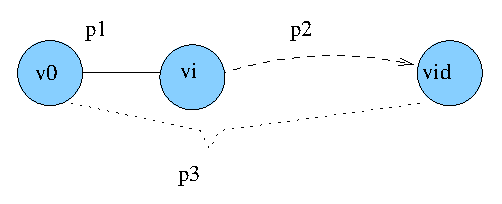
\includegraphics{rlogic/figures/induced_path1.eps}}
\end{psfrags}
%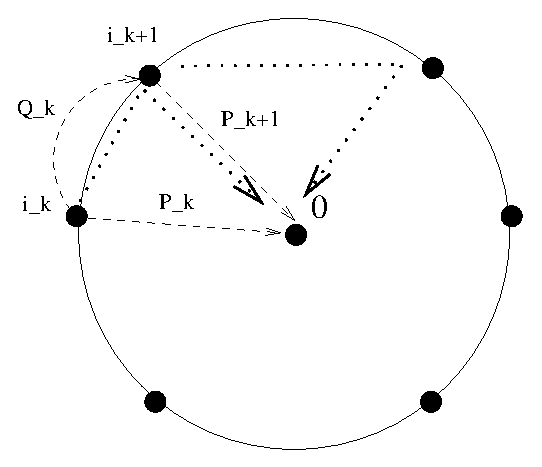
\epsfig{file=policy/figures/dw.eps,width=0.28\textwidth}
\caption[Illustration of an induced path.]{Illustration of an induced 
  path from $v_0$ to $d$, collectively induced by the selection of
  a route to $d$ at every node along the path.  The node $v_i$ may be
  immediately adjacent to $v_0$ (as shown), but it may also be several
  hops away.}
\label{fig:induced_path}
\end{figure}


\begin{defn}[Induced path]\label{defn:ipath}
Let $r_{v_j}(d)$ be the route that node $v_j$ selects en route to $d$
(\ie, it is a mapping $(d \rightarrow v_k)$ for some other $v_k\in G$.
Then, the {\em path induced} by route $r_{v_0}(d): (d \rightarrow v_i)$,
$P_{v_0}(r_{v_0}(d))$, is:
\[
P_{v_0}(r_{v_0}(d)) = \left\{\
\begin{array}{l}
\phi \textrm{ if $v_0$ has no route to $d$ }\\
v_0  \textrm{ if $v_0 \in d$}\\
%(v_0, P_{v_0}(r_{v_0}(v_i)), P_{v_i}(r_{v_i}(d))) \textrm{ otherwise }
(v_0, P_{v_1}(r_{v_1}(d))) \textrm{ otherwise }
\end{array}
\right.
\]
where $v_1$ is defined according to $r_{v_0}(v_i): (d \rightarrow v_1)$;
that is, $v_1$ is the next-hop node in $v_0$'s forwarding table for
destination $v_i$.
\end{defn}

\noindent
Figure~\ref{fig:induced_path} illustrates an induced path and its
constituent subpaths.  The node $v_i$ in the induced path may either be
adjacent to $v_0$ in $G$, or it may be several hops away.  When $v_i$ is
adjacent to $v_0$ in $G$, data traffic can reach $v_i$ from $v_0$ via a direct
IP link.  When $v_i$ is several hops away in $G$, however, $v_0$ must
rely on intermediate nodes to forward traffic to $v_i$.  In this case,
the nodes between $v_0$ and $v_i$ could 
use routes that induce paths that never even traverse $v_i$.
In other words, the path that is described by $(v_0,
P_{v_0}(r_{v_0}(v_i)))$ may traverse an intermediate node whose induced
path to $d$ does not traverse $v_i$.  To precisely
classify the types of paths for which 
this inconsistency does not arise, we define the notion of a consistent
path.

\begin{defn}[Consistent path]
An induced path $P_{v_0}(r_{v_0}(d)) = (v_0, \ldots v_n)$ to $d$ is consistent
if, (1)~for all $1 \leq i \leq n$, $P_{v_i}(r_{v_i}(d)) = (v_i, v_{i+1},
\ldots, v_n)$; (2)~$P_{v_0}(r(v_0(d)))$ contains $v_i$, where
$r_{v_0}(d): d \rightarrow v_i$.
\end{defn}

Consistent paths are an important class of paths because inconsistent
paths can sometimes give rise to forwarding loops.  A {\em forwarding
loop} is a special case of an inconsistent path where some intermediate
node's induced path includes a node that has already appeared on the
path.  

When $v_0$ and $v_i$ are not adjacent, ensuring that all intermediate
nodes select a route $(d\rightarrow v_i)$ will guarantee that an induced
path is consistent.  If an intermediate node selects some route
$(d\rightarrow v_j)$ where $v_i\neq v_j$, then the induced path to $d$
may never traverse $v_i$.  If, on
the other hand, the intermediate node selects a route $(d\rightarrow
v_i)$, then the induced path from that node to $v_i$ will be a subpath
of $P_{v_0}(r_{v_0}(v_i))$, assuming all nodes use the same function to
induce paths (\eg, if the induced path to $v_i$ is based on shortest
paths routing, as in an IGP).


%\subsection{Example: Paths and Routes in Internet Routing}

We now briefly discuss paths and routes in the context of BGP.  To
illustrate the distinction between routes and paths, we examine their
definitions within the context of BGP routing within a single AS.  In
this case, a {\em route} is of the form $(d \rightarrow v_i)$, where $d$
is an IP prefix and $v_i$ is the BGP ``next hop'' (a node that need not
be directly connected at the IP layer).  The {\em path} that traffic
ultimately takes from some node $v_j$ to the destination $d$, for which
$v_j$ has a route $(d \rightarrow v_i)$, depends on how connectivity is
established between $v_j$ and $v_i$.  If $v_j$ and $v_i$ are in two
different ASes, then they are typically directly connected.  If they are
in the same AS, however, it is common for $v_i$ to be the IP address of
an egress (or ``border'') router and for $v_j$ to be several IP hops
away.  The induced path between $v_j$ and $v_i$ may be determined by a
tunnel, by a shortest paths routing protocol, using static routes, etc.

If the induced path between $v_j$ and $v_i$ is not defined by a tunnel,
then the nodes between $v_j$ and $v_i$ will use their own routes for
forwarding data to $d$.  In this case, the induced path to $d$ is
actually determined by ``stitching together'' these constituent induced
paths.  If all nodes between $v_j$ and $v_i$ select routes that indicate
that traffic to $d$ should be sent via $v_i$, then the induced path
between $v_j$ and $v_i$ will be consistent.  Otherwise, the path could
be arbitrary; in fact, it might never traverse $v_i$.

\begin{figure}
\centering
\begin{psfrags}
\psfrag{v1}{{\LARGE $v_1$}}
\psfrag{v2}{{\LARGE $v_2$}}
\psfrag{v3}{{\LARGE $v_3$}}
\psfrag{v4}{{\LARGE $v_4$}}
\psfrag{v5}{{\LARGE $v_5$}}
\psfrag{d}{{\LARGE $d$}}
\psfrag{dr}{{\Large $(d \rightarrow v_5)$}}
%
%\hspace{-0.7in}
\resizebox{0.65\textwidth}{!}{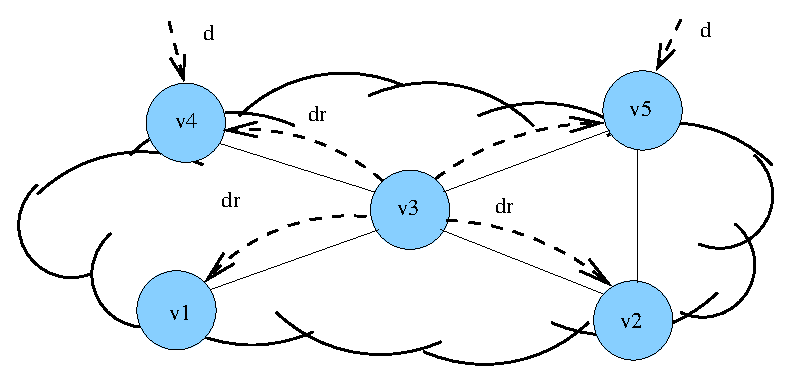
\includegraphics{rlogic/figures/path_route.eps}}
\end{psfrags}
%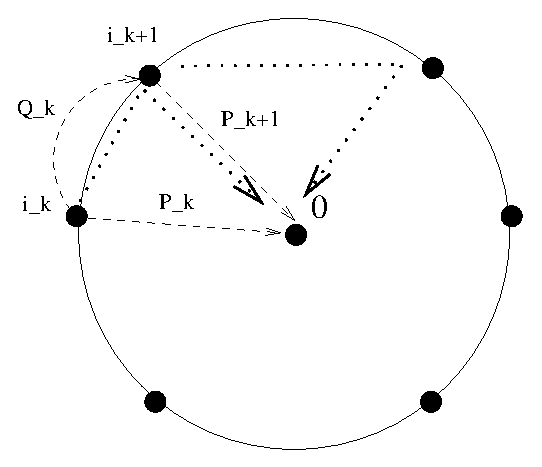
\epsfig{file=policy/figures/dw.eps,width=0.28\textwidth}
\caption[Paths and routes in BGP.]{An example that demonstrates how BGP
  routes induce paths.  Dashed lines are iBGP sessions from route
  reflectors to clients (\ie, $v_3$ is a route reflector, and the rest of
  the routers are its clients); route reflector operation is summarized
  in Section~\ref{sec:dissemination}.  Dashed lines show propagation of
  routes. Solid lines show IGP links; in this example, all links have a
  cost of $1$.  The routes at each node {\em induce} paths over the IGP
  topology. For example, the induced path from $v_2$ to $d$ is $(v_2,
  v_5, ...)$, the induced path from $v_1$ to $d$ is $(v_1, v_3, v_5,
  ...)$, etc.}
\label{fig:path_route}
\end{figure}

Figure~\ref{fig:path_route} shows an example that illustrates this
distinction.  In this example, all routers in the AS are clients of the
route reflector, $v_3$; solid lines show the edges in the IGP graph, and
all edges have a cost of $1$.  Suppose that $v_3$ learns two routes to
$d$ and selects the route that it receives from $v_5$.  In this case,
$v_3$ propagates that {\em route} (\ie, $(d \rightarrow v_5)$) to all of
its clients, as shown.   Using that route, each node ultimately uses a
different {\em path} to the egress router, $v_5$.  For example, $v_1$'s
shortest IGP path to $v_5$ is $v_1,v_3,v_5$, whereas $v_2$'s shortest
path to $v_5$ is $v_2, v_5$.  Even if a node, say $v_1$ selects a BGP
route with the ``next hop'' $v_5$, there is no guarantee that the
resulting {\em induced path} will traverse $v_5$.  If an additional
node, $v_6$, 
had been on the path between $v_1$ and $v_3$, and had instead selected a
route $(d\rightarrow v_4)$, then $v_1$'s path to $d$ through the AS
could have in fact been $v_1, v_6, v_4$.




%For the pursposes of our work, we assume that physical
%links and internal routing is operating correctly.  That is, we assume
%that a path exists between {\em any} source-destination pair where the
%source and destination are in the same AS.

\subsection{Policy}

A noteworthy aspect of Internet routing is that it is {\em policy-based}.
The job of the routing protocol is not to propagate complete
information about the topology, but to only propagate information about
paths that comply with the various economic and policy goals of each AS.
We must therefore qualify paths in the topology according to
those that comply with such these policies and those that do not.

\begin{defn}[Policy]\label{defn:policy}
A {\em policy} is a function $\P(s, v_{i-1},v_{i},v_{i+1},d) \rightarrow
(0,1)$, 
where $s$ is a source, $v_{i-1}$, $v_i$, and $v_{i+1}$ are 
nodes on a path $(v_0, v_1, \ldots, v_n)$, $d$ is a
destination, and $\P$ is defined as follows: 
\[
\P(s,v_{i-1},v_i,v_{i+1},d) = \left\{\
\begin{array}{l}
1\textrm{ if $i=0$ and $v_0$ forwards packets from source $s$ destined
  for $d$}\\ 
1\textrm{ if $0<i<n$ and $v_i$ forwards packets with source $s$ from
  $v_{i-1}$} \\ \textrm{\hspace*{0.2in} destined for $d$ via $v_{i+1}$}\\
1\textrm{ if $i=n$ and $v_n$ forwards packets with source $s$ destined
  for $d$}\\ 
0\textrm{ otherwise }
\end{array}
\right.
\]
\end{defn}

The function $\P(v_{i-1}, v_i, v_{i+1}, d)$ is not expressive enough to
capture all policies, but, as we will see, it is general enough to
capture the policies that are commonly expressed in Internet
routing.  Other routing protocols may require more expressive
policy functions. Our intent here is not to define a policy function
that captures all policies, but rather to allow us to define a
policy-conformant path in the context of Internet routing.

%A value of $0$ indicates that traffic
%should not be allowed to flow on any path from $s$ to $d$; a value of
%$1$ indicates that such a path is permissible.

\begin{defn}[Policy-conformant path]\label{defn:pcp}
A path $(v_0, v_1, v_2, \ldots, v_n)$ is policy-conformant for source $s$
and destination 
$d$ if $\P(s, v_{i-1}, v_i, v_{i+1},d) = 1$ for all $0 \leq i \leq n$.
\end{defn}

\noindent
For simplicity, we assume that paths for which the source,
destination, and all nodes in between the source and destination are in
the same AS are policy-conformant.  
%

\begin{figure}
\centering
\begin{psfrags}
\psfrag{X}{{\Large $X$}}
\psfrag{Y}{{\Large $Y$}}
\psfrag{Z}{{\Large $Z$}}
\psfrag{vx}{$v_X$}
\psfrag{vy1}{$v_i$}
\psfrag{vy2}{$v_j$}
\psfrag{vz}{$v_Z$}
\resizebox{0.9\textwidth}{!}{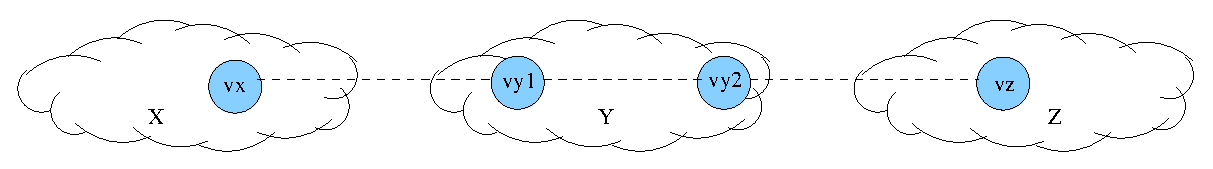
\includegraphics{rlogic/figures/policy_ex.eps}}
\end{psfrags}
\caption[Expressing policy-conformant paths at the AS-level in BGP.]{An example
  illustrating policy-conformant paths at the AS-level in BGP.}
\label{fig:policy_ex}
\end{figure}


%The policy function $\P$ allows an operator to restrict paths that do
%not conform to some policy by expressing $\P(v_{i-1},v_i,v_{i+1},d)$,
%where $v_{i-1}$, $v_i$, and $v_{i+1}$ are nodes in three different ASes.
Although the policy function is defined at the level of nodes, it is in
fact expressive enough to capture many AS-level policies that network
operators commonly want to express.  For example, suppose an operator
wants to express that AS $Y$ should not forward traffic between two other
ASes, $X$ and $Z$, for some destination $d$, as
pictured in Figure~\ref{fig:policy_ex}.  Recall that a path with some
nodes removed still constitutes a path.  As such, it is possible 
to express this policy in terms of the nodes in ASes $X$ and $Z$
along the path.  For example, in Figure~\ref{fig:policy_ex}, the policy can be
expressed as $\P(s, v_X, v_i, v_Z, d) = 0$.  In a more complicated
scenario, if AS $Y$ has multiple nodes that are adjacent to nodes in
ASes $X$ and $Z$, the AS-level policy would be
expressed as an enumeration over node-level policies.



\section{Route Validity}\label{sec:validity_def}

In this section, we motivate and describe {\em route validity}.
Informally, route validity says that any route that the routing protocol
propagates should correspond to a usable path in the topology.  Route
validity concerns the properties of the paths induced by the routes that
the routing protocol propagates.

\begin{defn}[Route validity]\label{defn:rv}
A route for a destination $d$ is valid if, and only if, the path induced
by the route (1)~is consistent, (2)~is policy-conformant for all sources
that use the route, and
(3)~terminates at $d$.  We say that a routing protocol satisfies route
validity if the protocol propagates only valid routes for all
destinations.
\end{defn}


\begin{figure}
\centering
\begin{psfrags}
%\epsfig{file=policy/figures/lemdr.eps,width=0.25\textwidth}
%
\psfrag{vi}{ $v_i$}
\psfrag{vid}{ $v_n \in d$}
\psfrag{vnd}{ $v_n \in d$}
\psfrag{vi1}{$v_{i-1}$}
\psfrag{v0}{$v_0$}
\psfrag{v1}{$v_1$}
\psfrag{dr}{$(d \rightarrow v_i)$}
\psfrag{d}{$d$}
%
%\hspace{-0.7in}
\resizebox{\textwidth}{!}{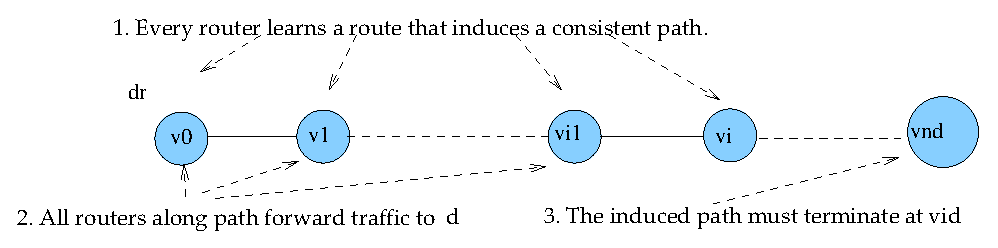
\includegraphics{rlogic/figures/rv_expl.eps}}
\end{psfrags}
%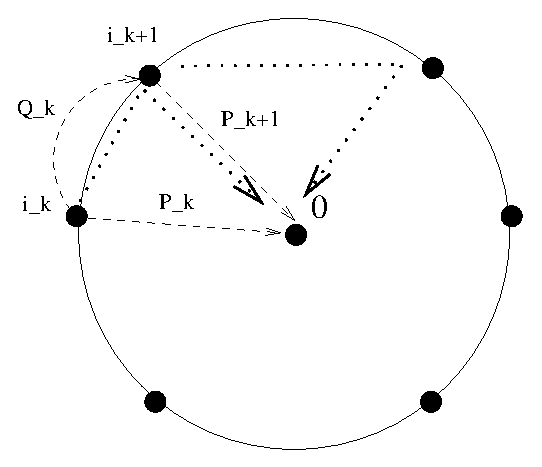
\epsfig{file=policy/figures/dw.eps,width=0.28\textwidth}
\caption[The conditions of route validity.]{The conditions of route
  validity.  A route is valid if it induces a consistent,
  policy-conformant path at every node along the path from $v_0$ to some
  $v_i \in d$.}
\label{fig:rv_expl}
\end{figure}


Figure~\ref{fig:rv_expl} illustrates the conditions of route validity.
The first condition of route validity enforces consistency
along the path between $v_0$ and the node $v_i$ towards which $v_0$
sends traffic en route to $d$.
%If all intermediate nodes
%between $v_0$ and $v_i$ have the same next-hop, $v_i$, then there can be
%no forwarding loops between $v_0$ and $v_i$.  
Furthermore, the induced path from $v_0$ to $v_i$ must be
policy-conformant; that is, every node along the path $(v_0, \ldots, v_i)$
must forward traffic from its predecessor to its next hop en route to
$d$.  Verifying policy conformance is difficult for
paths that traverse multiple ASes, because operators do not explicitly
specify the policy function $\P$.  The final condition says that the
path induced by the route must actually terminate at some node $v_n \in
d$.
%The final condition of route validity says that, once
%traffic reaches the node $v_i$, then that node also has a route to the
%destination that satisfies route validity.


%%%%%%%%%%%%%%%%%%%%%%%%%%%%%%%%%%%%%%%%%%%%%%%%%%%%%%%%%%%%

Because a source $v_0$ and a destination $d$ may be in different ASes,
guaranteeing that BGP satisfies route validity is difficult in practice.
Determining both the induced path to $d$ and determining whether that
path is policy-conformant requires knowledge of the configurations of
multiple ASes.  Fortunately, the properties of route validity (\ie,
consistency and policy-conformance) are composable.

\begin{observation}\label{obs:composable}
Composing a path by concatenating two consistent, policy-conformant
paths results in a new consistent, policy-conformant path.
\end{observation}

This observation implies that if the routing protocols in each AS en
route to a destination induce only consistent and policy-conformant
paths to some destination $d$, then BGP will only induce consistent,
policy-conformant paths for that destination $d$.  For the purposes of
this chapter, we assume that all paths are policy-conformant, because
detecting violations of policy are difficult to verify in practice; we will
return to this issue in Section~\ref{sec:validity}.  We also assume that
all eBGP sessions are point-to-point (\ie, immediately connected at the
IP layer), which is almost always the case in practice: service
providers typically apply policies at AS boundaries, rather than on
paths within an AS.  Finally, we assume that the IGP already satisfies
route validity; detecting route validity faults in internal routing
protocols is beyond the scope of this dissertation.



%% \begin{proof}
%% We must show that, when a route gives rise to a path where any $v_i$ and
%% $v_{i+1}$ are in different ASes, then the path that traverses the two
%% ASes still satisfies the conditions for route validity.  Since the path
%% segment $v_i, v_{i+1}$ is a point-to-point link, then $v_i$ selects the
%% route $(d \rightarrow v_{i+1})$, and the first condition is satisfied.
%% The third condition is satisfied by the inductive assumption.  
%% \end{proof}


Modulo policy-conformance, guaranteeing that BGP satisfies route
validity boils down to ensuring that iBGP always induces consistent
paths within each AS.  Guaranteeing this property is the focus of
the remainder of this section.  We first focus on how to guarantee that
``full mesh'' iBGP configurations (and protocol modifications that
would allow every
router to the complete set of ``best'' eBGP-learned routes) always
induce consistent paths; we 
then derive conditions on iBGP configurations that use route reflection
that guarantee that iBGP only induces consistent paths.

\subsection{Case \#1: Every router learns all ``best'' eBGP routes.}
\label{sec:mesh}

If different routers within an AS receive different sets of candidate
routes for some destination $d$, then the routers along a path from $v_0$
to $v_i$ may not ultimately select the route $(d \rightarrow v_i)$.  It
turns out that the default iBGP configuration, where every eBGP-speaking
router has an iBGP session with every other eBGP-speaking router in the
AS (\ie, a ``full mesh'' iBGP configuration, as described in
Section~\ref{sec:dissemination}, Figure~\ref{fig:fullmesh}) satisfies
route validity.

\begin{figure}
\centering
\begin{psfrags}
%\epsfig{file=policy/figures/lemdr.eps,width=0.25\textwidth}
%
\psfrag{v_i}{{\LARGE $v_i$}}
\psfrag{v_j}{{\LARGE$v_j$}}
\psfrag{a}{{\LARGE $a$}}
\psfrag{b}{{\LARGE$b$}}
\psfrag{s}{{\LARGE$v_0$}}
%
%\hspace{-0.7in}
\resizebox{0.5\textwidth}{!}{\includegraphics{rlogic/figures/fm_validity.eps}}
\end{psfrags}
%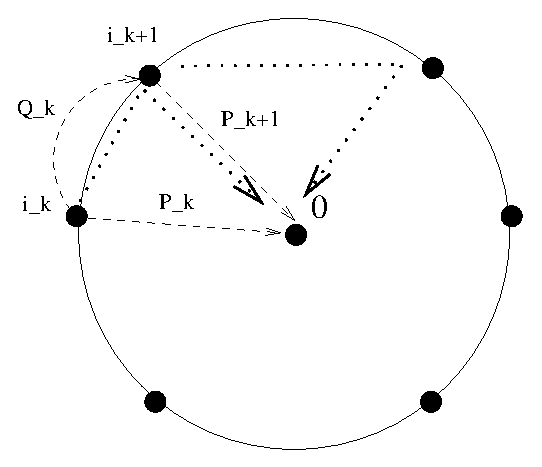
\epsfig{file=policy/figures/dw.eps,width=0.28\textwidth}
\caption[The main idea of the proof of
  Theorem~\ref{th:mesh}]{This figure illustrates the main idea of the proof of
  Theorem~\ref{th:mesh}.  Dashed lines represent iBGP sessions, and
  solid line represent IGP links.  If routes $a$ and $b$ do not have equal
  local preference, AS path length, origin type, or MED, then $v_0$,
  $v_i$, and $v_j$ will all select the same route.  If these attributes
  are equal for both $a$ and $b$, then $v_0$ selects either $a$ or $b$
  depending on whether $v_i$ or $v_j$ has a shorter IGP path.  If $v_j$
  selects route $a$ and $v_i$ selects route $b$, then $v_0$'s shortest IGP
  path to the next hop corresponding to the chosen route must be direct.}
\label{fig:fm_validity}
\end{figure}


\begin{theorem}\label{th:mesh}
If (1)~every router learns the BGP routes selected by the complete set of
eBGP-speaking routers, and
(2)~iBGP-speaking routers do not modify route attributes (\ie, local
preference, origin type, MED, or next hop), then 
all paths induced by iBGP (within the AS) will be consistent.
\end{theorem}

\begin{proof}
If each router eventually learns of the route selected by every
eBGP-speaking router, then there are two cases for any router $v_0$ in
the AS: either (1)~$v_0$ selects a route via a $v_i$ in a neighboring
AS, or (2)~$v_0$ selects a route via $v_i$ in the same AS, where $v_i$ is an
eBGP-speaking router and, hence, in turn selects a route such that
$v_{i+i}$ is in a neighboring AS.  The first case corresponds to a
point-to-point eBGP session; the second case corresponds to an iBGP
session where the route's next hop $v_i$ learned the route via a
point-to-point eBGP session but may be multiple IP hops away.  For the
proof of this theorem, we are only concerned with the latter case; we
rely on Observation~\ref{obs:composable} to ensure that iBGP induces
only consistent paths in neighboring ASes.

%% Route validity holds in the first case, because $v_i$ is in a
%% neighboring AS, and, by assumption, the remainder of the path is
%% consistent.  In the case where $v_i$ is in the same AS, the path $(v_0,
%% \ldots, v_i)$ may include multiple nodes (\ie, routers) in the same AS.
%% We know that $v_i$ selects a route that induces a consistent path
%% because $v_i$ selects a route from a neighboring AS.  

To show that iBGP induces only consistent paths within the AS, we show
that all routers on the path $(v_0, \ldots, v_i)$ select the route $(d
\rightarrow v_i)$, for any $v_i\in G$.  Because all eBGP-speaking
routers have an iBGP session with every other router in the AS, all
routers (and, in particular, all routers along the path $(v_0, \ldots,
v_i)$) learn the same set of ``best'' routes.  All of these routers
would thus select a route with the highest local preference, shortest AS
path length, lowest origin type, and lowest MED.

As a result, we know that all routers along the path $(v_0, \ldots,
v_i)$ select {\em some} iBGP learned route with the shortest IGP path
among candidate iBGP routes.  Suppose that some router on this path, say
$v_j$, selects a route other than $(d \rightarrow v_i)$, say $(d
\rightarrow v_k)$, because $(v_j, \ldots, v_k)$ has a shorter path cost
than $(v_j, \ldots, v_i)$.  Then, the nodes in $(v_0, \ldots, v_k)$ {\em
also} have a shorter IGP path cost than $(v_0, \ldots, v_i)$ and, hence,
all nodes in $(v_0, \ldots, v_{k-1})$ would also select $(d \rightarrow
v_k)$.
\end{proof}

A full mesh iBGP configuration can guarantee the first condition of
Theorem~\ref{th:mesh}.  Another approach to ensuring that every router
learns the set of routes selected by the complete set of eBGP-speaking
routers is to alter how route reflectors readvertise routes to their
clients.  By a similar argument as in the proof of
Theorem~\ref{th:mesh}, such a modification would cause iBGP to induce
only consistent paths.  Such a configuration not only guarantees
consistent paths, but it also prevents certain types of persistent route
oscillation (a pathology we examine in more detail in
Section~\ref{sec:safety_def})~\cite{Basu2002}. Unfortunately,
implementing such a configuration in practice requires modifying the
large deployed base of BGP routers.  Alternatively, an architecture such
as either the Routing Control Platform
(RCP)~\cite{caesar2004,feamster:fdna2004} or the recent proposal for
more versatile route reflectors~\cite{id-versatile-rr} could implement
this type of iBGP configuration.


%% \begin{defn}[RR-Reflect-All]
%% A route reflector configuration for an AS is {\em RR-Reflect-All} if all
%% route reflectors for that AS advertise all routes to a particular
%% destination (as opposed to simply the best route), and route reflectors
%% readvertise all routes with each other (\ie, path visibility is
%% satisfied among router reflectors).
%% \end{defn}

%% \begin{theorem}\label{th:rr_reflect}
%% If the route reflectors in an AS are configured according to {\em
%% RR-Reflect-All}, then all paths induced by iBGP are consistent.
%% \end{theorem}

%% \begin{proof}

%% In an {\em RR-Reflect-All} iBGP configuration, all routers ultimately
%% receive all routes to a destination $d$.  There are two cases:
%% (1)~there exists only one route that is better according to the first
%% four steps of the BGP route selection process (local preference, AS path
%% length, 
%% origin type, MED); (2)~there exists more than one route to $d$, and ties
%% between multiple candidate routes are broken after the first four steps.
%% In the first case, all routers will select that single route with common
%% next hop, so route validity is satisfied because every router selects
%% the same next hop.  In the second case, either a router $v_0$ selects a
%% route via its own eBGP session, if one exists (in which case route
%% validity is trivially satisfied again) or it selects a route that
%% traverses other routers in the same AS to reach the next hop $v_i$.
%% Because every router receives all routes to a destination, if some
%% router on the shortest path between $v_0$ and $v_i$ selects a route with a
%% next-hop other than $v_i$, then $v_0$ would have also selected the route
%% with that next hop, by the same argument in Theorem~\ref{th:mesh}.
%% \end{proof}





\subsection{Case \#2: Each router learns only some ``best'' eBGP routes}

If full mesh iBGP were the only intra-AS BGP configuration,
guaranteeing that iBGP satisfied route validity would be easy.
Unfortunately, as discussed in Section~\ref{sec:dissemination}, this
technique does not scale to large ASes because it requires $O(|R|^2)$
iBGP sessions, where $|R|$ is the number of routers in the AS.  Large
ASes typically use a 
technique called route 
reflection, where a single route reflector selects a route on behalf of
its client routers.


\begin{figure}
\begin{center}
\begin{psfrags}
\psfrag{RR1}{{\LARGE $RR_1$}}
\psfrag{RR2}{{\LARGE $RR_2$}}
\psfrag{C1}{{\LARGE $C_1$}}
\psfrag{C2}{{\LARGE $C_2$}}
\psfrag{d}{{\LARGE $d$}}
%\centering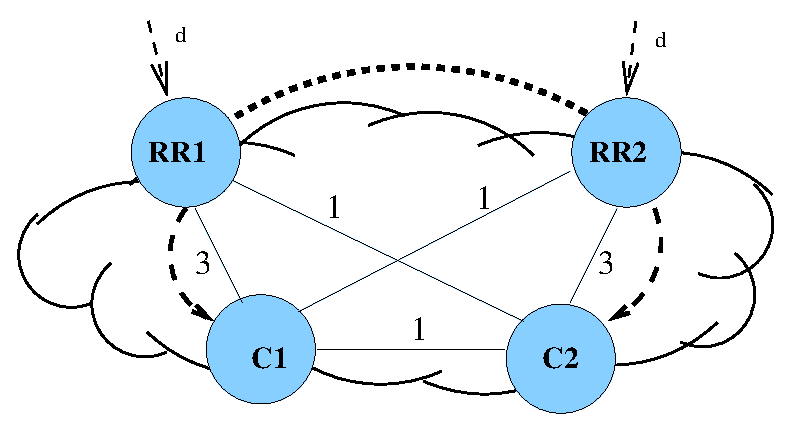
\epsfig{file=rlogic/figures/dube.eps,width=0.7\textwidth}
\resizebox{0.5\textwidth}{!}{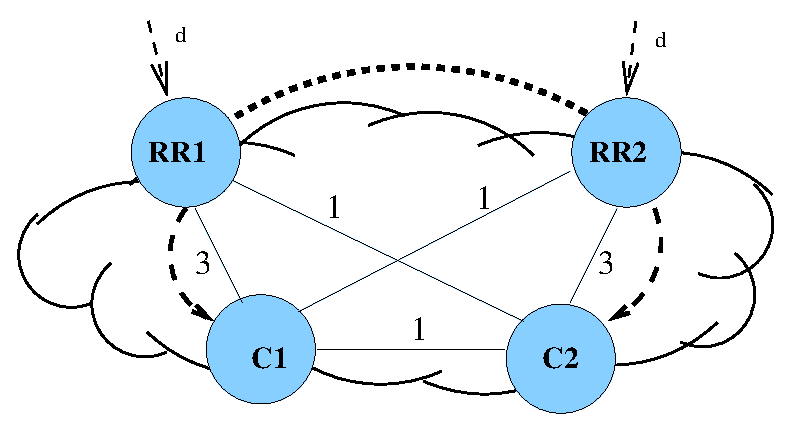
\includegraphics{rlogic/figures/dube.eps}}
\end{psfrags}
\end{center}
\caption[The interaction of IGP and route reflection may cause
  forwarding loops.]{The interaction of IGP and route reflection in iBGP
  may cause route validity violations resulting in forwarding
  loops~\cite{Dube99}. 
  Note that this topology satisfies path visibility but not route
  validity.  Dashed lines represent iBGP sessions; a directed edge
  indicates an iBGP sessions from a route reflector to its client.}
\label{fig:dube}
\end{figure}


Guaranteeing route validity in an iBGP topology with route reflectors is
not easy.  Previous work has observed that the interactions between the
IGP topology and an iBGP topology with route reflectors can give rise to route
validity violations~\cite{Dube99}.  Figure~\ref{fig:dube} shows one such
example.  Route reflectors $RR_1$ and $RR_2$ both receive a route to
destination $d$ and have clients $C_1$ and $C_2$ respectively.  Hence,
$C_1$ may receive and select the route $(d \rightarrow RR_1)$, and $C_2$
may receive and select the route $(d \rightarrow RR_2)$.  If the
shortest IGP path (\ie, the induced path) between $A$ and $RR_1$ is via
$B$, and the shortest 
IGP path between $B$ and $RR_2$ is via $A$, then traffic en route to $d$
that traverses either router $A$ or $B$ will be caught in a persistent
{\em forwarding loop}: that is, traffic destined for $d$ will never
reach $d$ but instead will repeatedly visit a cycle of two or
more nodes.  A forwarding loop is simply a special case of a route
validity violation.

Our goal is to detect whether a configuration of route reflectors and
clients induces only consistent paths with a simple algorithm that
examines only the static iBGP and IGP topologies.  One such sufficient
condition that guarantees this property requires that the iBGP topology
be {\em RR-IGP-Consistent}, defined as follows:

\begin{defn}[RR-IGP-Consistent]\label{defn:igp-consistent}
A route reflector configuration is {\em RR-IGP-Consistent} if, for all
nodes, every shortest IGP path between that node and its possible egress
nodes (\ie, the set of eBGP-speaking routers) traverses that node's
route reflector before any other node's route reflector and the egress
node's route reflector before the egress node itself.
\end{defn}
In previous work, Dube suggested placing route
reflectors on the shortest IGP path to their clients~\cite{Dube99}.  We
now prove that this condition guarantees that the iBGP configuration
will only induce consistent paths.  

\begin{theorem}\label{th:rr_safe}
If an iBGP configuration is {\em RR-IGP-Consistent}, then
all paths induced by iBGP are consistent.
\end{theorem}

\begin{proof}
Suppose not.  Then, there must exist a
destination $d$ and a path $P = (v_0, \ldots, v_n)$ for which some node $v_j$
between $v_0$ and $v_n$ selects a route $(d \rightarrow v_i)$, where $i
\neq n$.  There are two cases: (1)~$v_j$ is on the path from $v_0$ to the
route reflector of $v_0$; and (2)~$v_j$ is on the path from the route
reflector of $v_0$ to $v_n$.  

In the first case, if $v_0$ and $v_j$ select different next hops then, by
definition, they must be clients of different route reflectors.
By definition, then, the iBGP topology is not {\em RR-IGP-Consistent}.
%Then,
%it must be the case that either $v_0$'s path to $v_n$ goes through $v_j$'s
%route reflector before its own route reflector, or $v_j$'s path to $v_n$
%goes through $v_0$'s route reflector before its own route reflector.
%Either case implies that {\em RR-IGP-Consistent} is not satisfied.
The second case reduces to a similar argument as in
Theorem~\ref{th:mesh}: if $v_j$ selects a route with a next hop other
than $v_n$, then the route reflector of $v_0$ would have also learned that
route and selected it (otherwise, $v_j$ would not have been on the route
reflector's shortest path to $v_n$, by the same argument as in
Theorem~\ref{th:mesh}).
\end{proof}

Although this result is a helpful sufficient condition, it does not
guarantee that route validity will be satisfied when arbitrary links
fail, thus causing shortest IGP paths to change.  Designing an {\em
RR-IGP-Consistent} iBGP topology that is robust to link failures is a
difficult task.  Recent work has proposed using graph separators as a
way of efficiently placing route reflectors in an iBGP topology 
to guarantee that route validity is satisfied~\cite{Vutukuru2005}.  


%%%%%%%%%%%%%%%%%%%%%%%%%%%%%%%%%%%%%%%%%%%%%%%%%%%%%%%%%%%%

\section{Path Visibility}\label{sec:visibility_def}

Path visibility says that if there exists one or more policy-conformant
paths between two 
nodes, then the routing protocol should propagate routes that 
induce at least one of those paths.  Path visibility is an important
property for a number of reasons.  First, if a routing protocol
satisfies this property, then every node is guaranteed to have the
necessary information to reach all other nodes.
%Essentially, it states that the routing protocol is propagating
%enough information to allow any node to reach any other node for which
%it has a path in the underlying topology.  
%Second, as is evident from the
%theorems of Section~\ref{sec:validity_def}, an iBGP configuration must
%satisfy path visibility in order to satisfy route validity.

\begin{defn}[Path visibility]\label{defn:pv}
A routing protocol satisfies {\em path visibility} if, for all $v_0\in
V$ and for all destinations $d$, the existence of a policy-conformant
path $P = (v_0, \ldots, v_n)$ implies that $v_0$ learns a valid route
$(d \rightarrow v_j)$ for some $0 \leq j \leq n$.
\end{defn}

Path visibility states that if there is a policy-conformant
path from $v_0$ to $d$, then $v_0$ should learn {\em at least one} valid
route to $d$.  Note that the definition does not require $v_0$ to learn
all routes to $d$, nor does it require that $v_0$ learn the ``best''
route to $d$ by any metric.  Path visibility also does not require that
the route that $v_0$ learns correspond to the actual path that traffic
takes from $v_0$ to $d$.
%Although these might all be
%desirable properties, path visibility only requires the minimal
%conditions for correctness: as long as there is a policy-conformant path
%from $v_0$ to $d$, the routing protocol should propagate information that
%allows $v_0$ to send traffic to $d$.

By definition, path visibility violations result when some router fails
to propagate usable routes. These failures in route propagation 
range from the mundane (\eg, misconfigured filters that fail to
install or advertise routes for a policy-conformant path) to the subtle
(\eg, errors in iBGP configuration).

\begin{figure}
\begin{center}
\begin{psfrags}
\psfrag{R1}{{\LARGE $RR_1$}}
\psfrag{R2}{{\LARGE $RR_2$}}
\psfrag{R3}{{\LARGE $RR_3$}}
\psfrag{X}{{\LARGE $C_1$}}
\psfrag{Y}{{\LARGE $C_2$}}
\psfrag{Z}{{\LARGE $C_3$}}
\resizebox{0.6\textwidth}{!}{\includegraphics{rlogic/figures/ibgp_rr_pv.eps}}
\end{psfrags}
\end{center}
\caption[A simple iBGP topology that violates path visibility.]{A simple
  iBGP topology that violates path visibility.  Routes learned via eBGP
  at $RR_1$ or $C_1$ will not be propagated to $RR_3$ or $C_3$ (and vice
  versa).}
\label{fig:rl:ibgp_rr}
\end{figure}


Because of the way iBGP readvertises routes, an arbitrary iBGP
configuration is not guaranteed to satisfy path visibility.  In fact,
even the very 
simple iBGP topology in Figure~\ref{fig:rl:ibgp_rr} does not satisfy
path visibility: if the route reflector $RR_1$ (or its client, $C_1$)
receives a route for some destination via an eBGP session, then neither
$RR_3$ nor $C_3$ will receive a route to the destination, and vice
versa.  


Path visibility is important because it ensures that, if the network
remains connected at lower layers, the routing protocol does not create
any new network partitions.  Path visibility also reduces the likelihood of
suboptimal routing.  For example, in Figure~\ref{fig:rl:ibgp_rr}, even if
all clients learned {\em some} route to the destination via eBGP, the
clients would not be guaranteed to discover the {\em best} route to the
destination (\eg, if a client of the route reflector on the far left
learned a route with a shorter AS path, neither the route reflector on
the far right nor its clients would learn it).  As such, it is important
that an AS's iBGP configuration satisfy path visibility.  In the
remainder of this section, we derive the constraints on the iBGP
configuration that must be satisfied to guarantee path visibility.  We
first consider iBGP topologies that do not employ route reflection.


\begin{theorem}\label{th:mesh_visibility}
For an iBGP topology without route reflectors,
satisfying path visibility requires a full mesh iBGP configuration.
%that every router have an iBGP
%session with every router that may learn a route via eBGP (\ie, all
%routers are ``fully meshed'' with the eBGP-speaking routers).
\end{theorem}

\begin{proof}
Consider a router $v_i$, which learns a route $r$ for some destination $d$ via
eBGP, and a router $v_0$ within the same AS that does not have an iBGP
session to $v_i$.  Then, $v_i$ will readvertise $r$ to the routers to which
it has iBGP sessions, but none of those routers will advertise the route
to $v_0$, because they all learned the route via iBGP.
\end{proof}

%% Note that an iBGP configuration without route reflectors does {\em not}
%% require every router to have an iBGP session with every other router (as
%% is commonly stated): the routers that do not receive any routes to a
%% destination via eBGP need not have iBGP sessions with each other.


In large networks, a route reflector may itself be a client
of another route reflector.  Any router may also have ``normal'' (\ie,
peer) iBGP sessions with other routers.  We use the set of
reflector-client relationships between routers in an AS to define a
graph $\I$, where each router is a node and each session is either a
directed or undirected edge: a client-reflector session is a directed
edge from client to reflector, and peer iBGP sessions are undirected
edges. We say that $\I$ is {\em acyclic} if $\I$ has no sequence of
directed and undirected edges that form a cycle.  In typical iBGP
hierarchy designs, $\I$ is acyclic (previous work states that $\I$ should
be acyclic to prevent protocol oscillations~\cite{Griffin2000}---and it
is a good design decision anyway---although
we will see in Section~\ref{sec:safety_def} that this constraint is
unnecessary).  We now define the topological constraints on $\I$ to
guarantee path visibility.


\begin{theorem}\label{thm:vis}
Suppose that the graph defined by an AS's iBGP relationships, $\I$, is
acyclic.  Then, $\I$ does not have a signaling partition if, and only
if, the eBGP-speaking routers that are not route reflector clients form
a clique. 
\end{theorem}

\begin{figure}
\centering
\begin{psfrags}
\psfrag{c0}{}
\psfrag{c1}{}
\psfrag{c2}{}
\psfrag{RR0}{$RR_0$}
\psfrag{RR1}{$RR_1$}
\psfrag{RR2}{$RR_2$}
\resizebox{0.5\linewidth}{!}{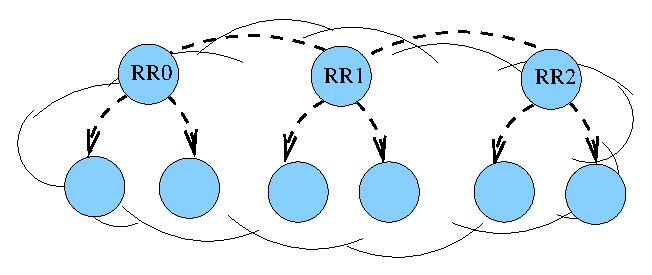
\includegraphics{rlogic/figures/path_vis_ibgp.eps}}
\end{psfrags}
\caption[The main idea of the proof of
  Theorem~\ref{thm:vis}.]{Illustrating the main idea of the proof of
  Theorem~\ref{thm:vis}.}
\label{fig:path_vis_ibgp}
\end{figure}

\begin{proof}
Call the set of routers that are not reflector clients the ``top layer''
of $\I$.  If the top layer is not a clique, then there are two routers
with no iBGP session between them, such that no route learned via eBGP
at $RR_i$ will ever be disseminated to $RR_j$, since no router
readvertises an iBGP-learned route (\eg, $RR_0$ and $RR_2$ in
Figure~\ref{fig:path_vis_ibgp}), and vice versa.  Furthermore, no route that
is learned via eBGP at any of $RR_i$'s clients will be disseminated to
$RR_j$ or $RR_j$'s clients, and vice versa.

Conversely, suppose the top layer is a clique. Observe that if a route
reflector has a route to the destination, then all of its clients have a
route as well.  Thus, if every router in the top layer has a route, all
routers in the AS will have a route.  If any router in the top layer
learns a route through eBGP, then all the top layer routers will hear of
the route (because the top layer is a clique).  Alternatively, if no
router at the top layer hears an eBGP-learned route, but some other
router in the AS does, then that route propagates up a chain of route
reflectors (each client sends it to its reflector, and the reflector
sends it on all its iBGP sessions) to the top layer, from there to all
the other top-layer routers, and from there to the other routers in the
AS.
\end{proof}

The results in this section suggest that path visibility can be
guaranteed by checking relatively simple constraints on the iBGP
topology, which can be determined by analyzing the static configuration
files alone.  Although, in the long term, architectural changes could be
made to guarantee that no configuration ever violates path
visibility~\cite{id-versatile-rr, caesar2004, feamster:fdna2004},
relatively simple checks against routing configuration can guarantee
path visibility today (as we will see in Chapter~\ref{chap:rcc}). 



\section{Safety}\label{sec:safety_def}

%In this section, we discuss properties related to improving
%predictability in Internet routing: {\em safety} and {\em determinism}.
Violations of safety can cause the routing protocol
to continually send routing updates that do not reflect changes in the
underlying topology.  We provide an informal definition of
safety and defer a formal definition to Chapter~\ref{chap:policy}
(Definition~\ref{def:safety}).

\begin{defn}[Safety]
A routing protocol satisfies {\em safety} if and only if, given no
changes to available paths after time $t_0$, then, at some finite time
$t_s > t_0$, each node $v\in G$ selects some route $r$ and does not
select a route $r'\neq r$ for any $t > t_s$.
\end{defn}

Safety is an important property because it guarantees that changes in
{\em routes} (\ie, routing update messages) correspond directly to
changes in available {\em paths}.  This invariant is important for
several reasons.  First, if the routing protocol causes routers to
change routes unnecessarily (\ie, when the paths are in fact stable),
the protocol itself may cause performance degradations, such as lost or
reordered packets.  Second, if routing changes do not correspond to
changes in the actual topology, then debugging the cause of an
oscillation becomes more difficult, because an operator cannot determine
whether routing changes reflect problems with infrastructure (\eg, flaky
or failing equipment) or the routing protocol itself.

Safety problems arise for two reasons:
\begin{enumerate}
\itemsep=-1pt
\item Conflicting route selections within the same AS, caused by
  interactions between BGP route attributes and the IGP (iBGP safety).
\item Conflicting rankings, caused by conflicting policies between
  ASes (eBGP safety).
\end{enumerate}
In both cases, guaranteeing safety is hard.  The
rest of this section focuses on the constraints for guaranteeing safety
in iBGP.  Guaranteeing that eBGP satisfies safety requires either 
knowing the rankings of ASes across the {\em global} Internet (not
a realistic requirement, because ASes typically insist on keeping their
rankings private) or placing restrictions on how each AS can specify
rankings and filters.  This problem is the focus of
Chapter~\ref{chap:policy}.

Safety violations in iBGP occur because BGP's route selection process
(as described in Table~\ref{tab:background:decision},
Section~\ref{sec:bg:route_selection}) does 
not satisfy {\em determinism}.  Determinism essentially says that the
route each router ultimately selects should not depend on either 
(1)~the presence or absence of routes
that would not be selected in the first place or
(2)~the
order in which messages arrive.  We formally define
determinism and explain why guaranteeing this property is difficult in
practice.
\begin{defn}[Selection function]
A selection function at router $r$, $\lambda_r$, takes as input a set of
routes $R_d = \{r_1, \ldots, r_n\}$ for some destination $d$ and produces
a single route $r_i \in R_d$.  The route $r_i$ is often called the
router's ``best route'' to $d$.
\end{defn}

\begin{defn}[Determinism]\label{def:determinism}
A routing protocol satisfies {\em determinism} for destination $d$ if,
for all routers $r$, if $r$ has a set of routes $R_d$ to $d$,
$\lambda_r(R_d)$ satisfies the following two properties:
\begin{enumerate}
\itemsep=-1pt
\item $\lambda_r(R_d) = \lambda_r(R'_d)$, where $R'_d$ is any subset of
  $R_d$ that contains $\lambda_r(R_d)$, and
\item $\lambda_r(R_d)$ does not depend on the order in which the routes
  in $R_d$ arrived at router $r$.
\end{enumerate}
Determinism depends only on the
selection function, $\lambda_r$, for all routers $r$.  Thus, we may also
discuss a single selection function, $\lambda_r$, in terms of whether it
satisfies determinism.
%% Let $\Sigma(R_d) = \{\sigma_1(R_d), \ldots, \sigma_{n!}(R_d)\}$ as
%% the set of all permutations of $R_d$ (\ie, the set of all possible
%% arrival orders for the candidate routes to $r_d$.
%% %
%% Let $T(R_d) = \{t_1(R_d), \ldots, t_{2^n}(R_d)\}$ be the set of all
%% subsets of $R_d$. 
%% %
%% Then, determinism is satisfied if and only if, for all $r_i \in
%% R_d$, $\lambda_r(R_d) = r_i \Rightarrow (r_i \in t_i(R_d) \Rightarrow
%% \lambda_r(\sigma_i(t_i(R_d))) = r_i)$, for all $\sigma_i \in \Sigma(R_d),
%% t_i \in T(R_d)$.
\end{defn}

%% In other words, if a router $r$ selects a certain route as its best
%% route from a set of candidate routes, then it should {\em always} select
%% that route if other routes are removed from that candidate set, and it
%% should always select that route regardless of the order in which
%% those routes arrive at router $r$.
Determinism is important for predictability; moreover, as the following
observation shows, violations of determinism can induce safety
violations, even when the selection function of only one router violates
determinism.


\begin{figure}
\centering
\begin{psfrags}
\psfrag{R1}{{\Large $R_1$}}
\psfrag{R2}{{\Large $R_2$}}
\psfrag{1}{$1$}
\psfrag{2}{$2$}
\psfrag{A}{$A$}
\psfrag{B}{$B$}
\psfrag{C}{$C$}
\psfrag{r1}{$\lambda_{R_1}(\{A,B\}) = A$; $\lambda_{R_1}(\{A,C\}) = C$}
\psfrag{r2}{$\lambda_{R_2}(\{A,B, C\}) = C$;  $\lambda_{R_2}(\{B,C\}) = B$}
\psfrag{A/P}{$A/\phi$}
\psfrag{B/C}{$B/C$}
%
\hspace{-0.4in}
\resizebox{0.7\textwidth}{!}{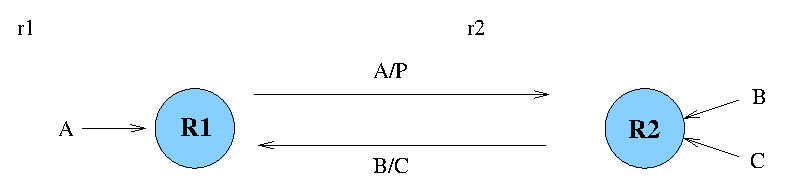
\includegraphics{rlogic/figures/det_a.eps}}
\end{psfrags}
%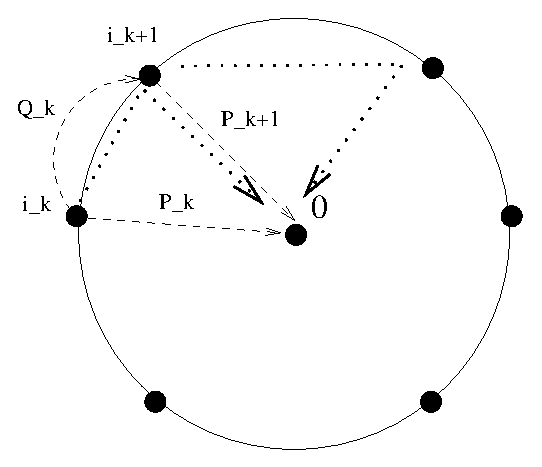
\epsfig{file=policy/figures/dw.eps,width=0.28\textwidth}
\caption[How determinism violations can cause safety
  violations.]{$\lambda_{R_2}$ does not satisfy determinism.  This violation
  can causes a safety violation.}
\label{fig:determinism}
\end{figure}


\begin{figure}
\centering
\begin{psfrags}
\psfrag{R1}{{\Large $R_1$}}
\psfrag{R2}{{\Large $R_2$}}
\psfrag{R3}{{\Large $R_3$}}
\psfrag{1}{$1$}
\psfrag{2}{$2$}
\psfrag{3}{$3$}
\psfrag{A}{$A$}
\psfrag{B}{$B$}
\psfrag{C}{$C$}
\psfrag{r1}{$\lambda_{R_1}(\{A,C\}) = C$;  $\lambda_{R_1}(\{A,B\}) = A$}
\psfrag{r2}{$\lambda_{R_2}(\{A,B, C\}) = C$;  $\lambda_{R_2}(\{B,C\}) = B$}
\psfrag{A/P}{$A/\phi$}
\psfrag{B/C}{$B/C$}
%
\hspace{-1.5in}
\resizebox{0.7\textwidth}{!}{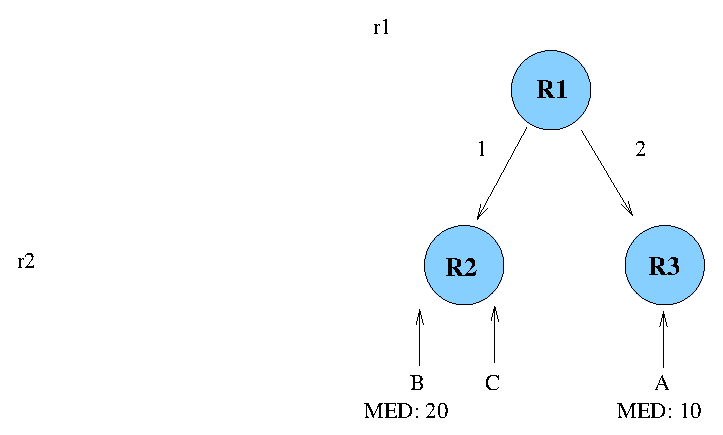
\includegraphics{rlogic/figures/det_b.eps}}
\end{psfrags}
%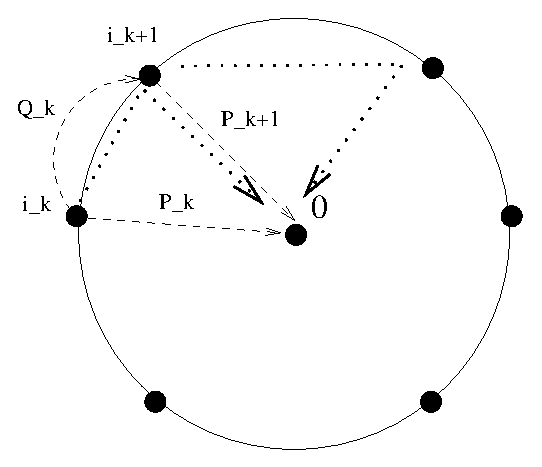
\epsfig{file=policy/figures/dw.eps,width=0.28\textwidth}
\caption[Instantiation of Figure~\ref{fig:determinism} in a BGP
  configuration.]{Instantiation of Figure~\ref{fig:determinism} in a BGP
  configuration.  Router $1$ is a route reflector with two clients, $R_2$
  and $R_3$.  Costs on edges are IGP path costs.  Router $R_2$ prefers route
  $B$ over route $C$ due to a tiebreak.}
\label{fig:determinism_bgp}
\end{figure}

\begin{observation}
If the selection function of even one router, $\lambda_r$, violates
determinism, then the routing protocol may also violate safety.
\end{observation}

\noindent
The following example illustrates this point.

\begin{example}\label{ex:med_det}
Consider Figure~\ref{fig:determinism}.  Router $R_1$ selects route $A$
given the choices $\{A, B\}$ and selects route $C$ given choices
$\{A,C\}$. This selection function satisfies determinism.
On the other hand, router $R_2$'s selection function violates determinism:
$\lambda_{R_2}(\{A,B,C\}) = C$, but $\lambda_{R_2}(\{B,C\}) = B$.  The
interaction of the two selection functions creates the following
oscillation: 
\begin{enumerate}
\itemsep=-1pt
\item Router $R_1$ receives only route $A$, selects it, and
  advertises this route to router $R_2$.
\item Router $R_2$ has received $\{A,B,C\}$, selects
  route $C$, and advertises it to router $R_1$.
\item Router $R_1$ has received $\{A,C\}$, selects
  route $C$, and sends a withdrawal ($\phi$) for route $A$ to router
  $R_2$. 
\item Router $R_2$ selects $B$ from the set $\{B,C\}$ and advertises it to
  router $R_1$, implicitly withdrawing route $C$. 
\item Router $R_1$ now has to select a route from the set $\{A,B\}$, selects
  route $A$, and advertises it to router $R_2$.
\end{enumerate}
This process repeats forever, violating safety.
\end{example}

\subsection{Determinism Violations in BGP: The MED Attribute}

It turns out that the above scenario can occur in BGP, because the MED
attribute causes each router's selection function to violate
determinism.  The addition of a third router, as shown in
Figure~\ref{fig:determinism_bgp}, gives rise to the oscillation from the
previous example.  In this case, router $R_1$ is a route reflector for
two clients: routers $R_2$ and $R_3$, with IGP costs as shown.  Routes
$A$ and $B$ are advertised by the same AS, and route $A$ has a lower MED
value (and, hence, is preferred to $B$).  In this setup, the selection
functions are exactly as described 
in the from Figure~\ref{fig:determinism}: when router $R_2$ learns $\{A,B,C\}$,
route $B$ is eliminated due to MED, and route $C$ is selected because it
is an eBGP-learned route.  When router $R_2$ learns only $\{B,C\}$, on
the other hand, it prefers route $B$ over route $C$ due to the router ID
tiebreak.  Similarly, router $R_1$ prefers route $C$ over route $A$ due
to IGP, but router $A$ over router $B$ due to MED.  The routing system
in this example oscillates in the same fashion as the one shown in
Figure~\ref{fig:determinism}. 

As the above example shows, the interaction between the MED attribute
and route reflection can cause BGP to violate safety.  Note that this
example satisfies the guidelines that were specifically proposed to
avoid these types of oscillations~\cite{rfc3345}.  Even though not all
safety violations are caused by violations of determinism, eliminating
BGP's determinism problem can eliminate all oscillations that do not
involve cyclic preferences over routes caused by setting the local
preference attribute.  Specifically, by making the MED attribute
comparable across {\em all} routes, rather than just those from the same
AS, each router's selection function can be made to satisfy determinism.
We now formally show this result.

\begin{lemma}\label{lem:det_med}
If a router's selection function compares the MED attribute across all
routes to a destination (rather than just across those from the same
neighboring AS), then its selection function satisfies determinism.
\end{lemma}

\begin{proof}
We must show that if the router's selection function compares the MED
attribute across all routes to a destination then: (1)~the route it
selects does not change when any route is removed from that set; and
(2)~the route it selects does not depend on the order in which the
router receives them.

When a router compares the MED attribute across all routes to a
destination, then all routes to a destination can be totally ordered.
Specifically, all routes can be sorted by local preference.  Each set of
routes with equal local preference can be sorted from shortest AS path
length to longest, and so forth.  Thus, the set of routes to a
destination can 
be totally ordered, and removing a route from that set that is not the
most preferred in the total ordering will not change the most preferred
route, since that route must have had a lower local preference, longer
AS path length, higher origin type, lower MED, etc.  

We must also show that the route a router $r$ selects, $\lambda_r(R_d)$,
does not depend on the order that $r$ receives the routes in $R_d$.
%Define two message arrival orders, $\sigma_i(R_d)$ and $\sigma_j(R_d)$,
%and suppose that $\lambda_r(\sigma_i(R_d)) = \rho_i \in R_d$, but
%$\lambda_r(\sigma_j(R_d)) = \rho_j \in R_d$, where $\rho_i \neq \rho_j$.
We know that the routes in $R_d$ are totally ordered, which means that
there is a preference relation between any two routes $\rho_i$ and
$\rho_j$ that is consistent for {\em any} subset of $R_d$ that contains
both $\rho_i$ and $\rho_j$.  We also know that $\lambda_r(R_d)$ will
ultimately select the route that is most preferred in that total
ordering.  Suppose that most preferred route is $\rho_i$.  When $\rho_i$
arrives, $r$ will select $\rho_i$ and continue to select it even after
other routes arrive.  Thus, if $\rho_j$ arrives before $\rho_i$, then
the router will not continue to select $\rho_j$ after $\rho_i$ arrives,
since $\rho_i$ is strictly better than $\rho_j$ in the total ordering.
Similarly, if $\rho_j$ arrives after $\rho_i$, then $r$ will continue to
select $\rho_i$, since it is better than $\rho_j$ in the total ordering.
\end{proof}

We explore how comparing the MED attribute across all routes affects
protocol operation, as well as how this might be done in practice, in
Section~\ref{sec:sandbox:med_disc}.  In short, the primary benefit of
making the route selection function deterministic is that a set of
routers {\em 
within a single AS} may violate safety if determinism is not
satisfied.  Although determinism prevents safety violations such as
those shown in Figures~\ref{fig:determinism}
and~\ref{fig:determinism_bgp}, it does not prevent {\em all} violations
of safety.  For that, we require a stronger notion of determinism, which
we call {\em egress determinism}.


\subsection{Egress Determinism Violations in BGP: Route Reflection}

Even if determinism is satisfied, an AS's iBGP topology can still cause
a routing protocol to violate
safety.  In particular, we can construct an oscillation that
involves the interaction between an AS's route reflector topology and
its IGP topology.  To better understand this interaction, we first
define the notion of {\em egress determinism}.  Egress determinism is a
stronger condition than determinism, as shown in
Figure~\ref{fig:determinism_venn}; essentially, it states that, given a
set of routes learned at {\em any} egress router in the AS, a router's
preference between any pair of those routes should not depend on either
the order in which those routes arrive or the presence or absence of
other routes.  Egress determinism implies determinism, but it also
states that every router's selection function should satisfy determinism
for all routes learned at {\em any} router in the AS, not just those
learned locally at that router.

\begin{figure}
\centering
\begin{psfrags}
\resizebox{0.4\textwidth}{!}{\includegraphics{rlogic/figures/det_venn.eps}}
\end{psfrags}
%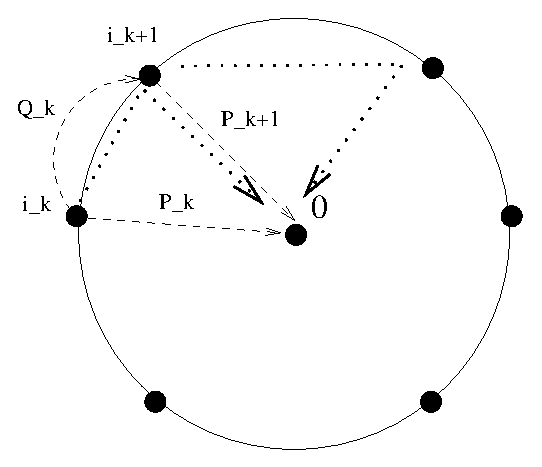
\epsfig{file=policy/figures/dw.eps,width=0.28\textwidth}
\caption[The relationship between determinism, egress determinism, and
  safety.]{The relationship between determinism, egress determinism, and
  safety.} 
\label{fig:determinism_venn}
\end{figure}


\begin{defn}[Egress Determinism]\label{def:egress_determinism}
Let $E_d$ be the set of routes for destination $d$ learned at {\em any}
router in the AS.  Then, a routing protocol satisfies {\em egress
determinism} for destination $d$ if $\lambda_r(E_d)$ satisfies the
following two properties:
\begin{enumerate}
\itemsep=-1pt
\item $\lambda_r(E_d) = \lambda_r(E'_d)$, where $E'_d$ is any subset of
  $E_d$ that contains $\lambda_r(E_d)$, and
\item $\lambda_r(E_d)$ does not depend on the order in which the routes
  in $E_d$ arrived at router $r$.
\end{enumerate}
\end{defn}

\begin{figure}
\centering
\begin{psfrags}
%
\psfrag{x}{{\LARGE $x$}}
\psfrag{y}{{\LARGE$y$}}
\psfrag{z}{{\LARGE $z$}}
\psfrag{X}{{\LARGE $X$}}
\psfrag{Y}{{\LARGE $Y$}}
\psfrag{Z}{{\LARGE $Z$}}
\psfrag{R1}{{\LARGE $R_1$}}
\psfrag{R2}{{\LARGE $R_2$}}
%
%\hspace{-0.7in}
\resizebox{0.6\textwidth}{!}{\includegraphics{rlogic/figures/det_violation_rr.eps}}
\end{psfrags}
%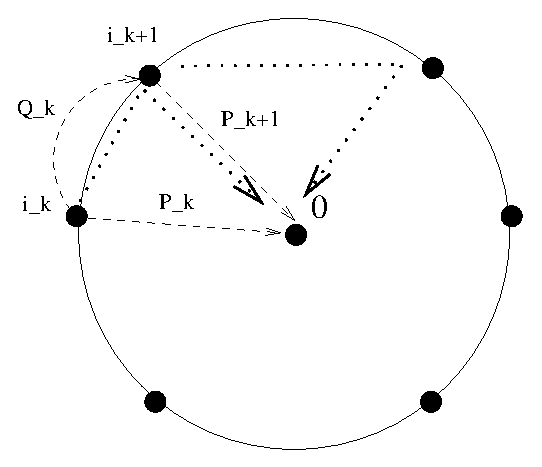
\epsfig{file=policy/figures/dw.eps,width=0.28\textwidth}
\caption[The interaction of IGP and iBGP can cause a violation of egress
  determinism.]{The interaction of IGP and iBGP can cause a violation of egress
  determinism. $\lambda_{R_1}$ is equal to either $x$ or $y$ depending
  on whether $z \in E_d$.}
\label{fig:det_violation_rr}
\end{figure}

Note that egress determinism is a stronger condition than determinism
because it states
properties that $\lambda_r$ must satisfy over the set of routes learned
by all routers in the AS, not just the routes learned at $r$.

If every router in the AS always learned all routes in $E_d$, then
violations of egress determinism would never cause oscillations: given a
fixed set of routes $E_d$, every router would always see that set and
select the same route.  In an iBGP topology with route reflectors,
however, most routers will see some subset of $E_d$, which means that
violations of egress determinism may cause safety violations.  Consider
Figure~\ref{fig:det_violation_rr}: $X$ is a route reflector client of
$R_1$, and $Y$ and $Z$ are clients of route reflector $R_2$. Suppose
that routers $X$, $Y$, and $Z$ all learn routes for some destination $d$
with equal local preference, AS path length, origin type, and MED
attributes, causing routers within the pictured AS to resort to
preferring eBGP routes over iBGP routes, and, that being equal, to
prefer routes with the shortest IGP path cost.  If $E_d = \{x,y,z\}$,
then $\lambda_{R_1}(E_d) = x$: $R_2$ selects $z$ due to its shorter IGP
path cost to the next hop, and $R_1$, having learned $x$ and $z$,
selects route $x$.  If, on the other hand, $E_d = \{x,y\}$, then
$\lambda_{R_1}(E_d) = y$: $R_2$ selects $y$, and $R_1$, having learned
both $x$ and $y$, selects $y$ due to the shorter IGP path cost. Thus,
the first condition of egress determinism is violated.

\begin{figure}
\centering
\begin{psfrags}
%
\psfrag{R1}{{\LARGE $R_1$}}
\psfrag{R2}{{\LARGE $R_2$}}
\psfrag{R3}{{\LARGE $R_3$}}
\psfrag{x}{{\LARGE $x$}}
\psfrag{y}{{\LARGE $y$}}
\psfrag{z}{{\LARGE $z$}}
\psfrag{r1}{{\LARGE $\lambda_{R_1}(\{x,y\}) = y$;
    $\lambda_{R_1}(\{x,y,z\}) = x$}}
\psfrag{r2}{{\LARGE $\lambda_{R_2}(\{x,z\}) = z$;
    $\lambda_{R_2}(\{x,y,z\}) = x$}} 
\psfrag{r3}{{\LARGE $\lambda_{R_3}(\{y,z\}) = z$;
    $\lambda_{R_3}(\{x,y,z\}) = y$}}
\psfrag{x/y}{{\LARGE $x/y$}}
\psfrag{y/z}{{\LARGE $y/z$}}
\psfrag{x/z}{{\LARGE $x/z$}}
%
\hspace{-0.7in}
\resizebox{0.85\textwidth}{!}{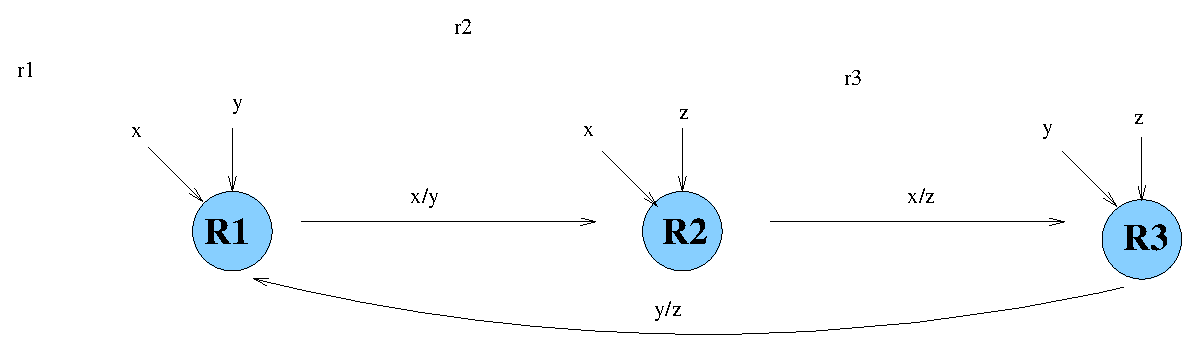
\includegraphics{rlogic/figures/abstract_sd.eps}}

\end{psfrags}
%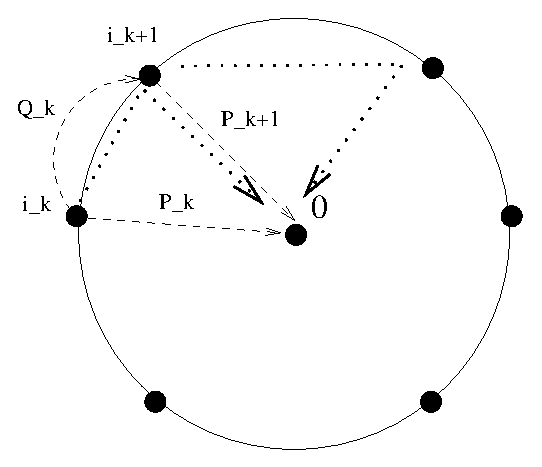
\epsfig{file=policy/figures/dw.eps,width=0.28\textwidth}
\caption[Egress determinism violations can cause safety
  violations.]{Violations of egress determinism can also cause the
  routing protocol to violate safety.}
\label{fig:abstract_sd}
\end{figure}


Like determinism violations, egress determinism violations can cause the
routing protocol to violate safety.  Consider three routers whose
selection functions violate egress determinism, as shown in
Figure~\ref{fig:abstract_sd}; $R_1$'s selection function is identical to
that in Figure~\ref{fig:det_violation_rr}. Each router prefers one route
or the other depending on the presence or absence of a third route.  In
this case, there is no stable assignment of routes $x$, $y$, and $z$ to
routers $R_1$, $R_2$, and $R_3$.  For example, if $R_1$ selects $x$,
then $R_2$ selects $z$ and $R_3$ selects $y$, prompting $R_1$ to select
$y$, and so on.  This very scenario can be realized in BGP today if
three routers' route selection functions fail to satisfy egress
determinism, as shown in Figure~\ref{fig:sd_violation_rr_osc}.


\begin{figure}[t]
\centering
\begin{psfrags}
%
\psfrag{x}{{\LARGE $x$}}
\psfrag{y}{{\LARGE$y$}}
\psfrag{z}{{\LARGE $z$}}
\psfrag{X}{{\LARGE $X$}}
\psfrag{Y}{{\LARGE $Y$}}
\psfrag{Z}{{\LARGE $Z$}}
\psfrag{R1}{{\LARGE $R_1$}}
\psfrag{R2}{{\LARGE $R_2$}}
\psfrag{R3}{{\LARGE $R_3$}}
%
%\hspace{-0.7in}
\resizebox{0.6\textwidth}{!}{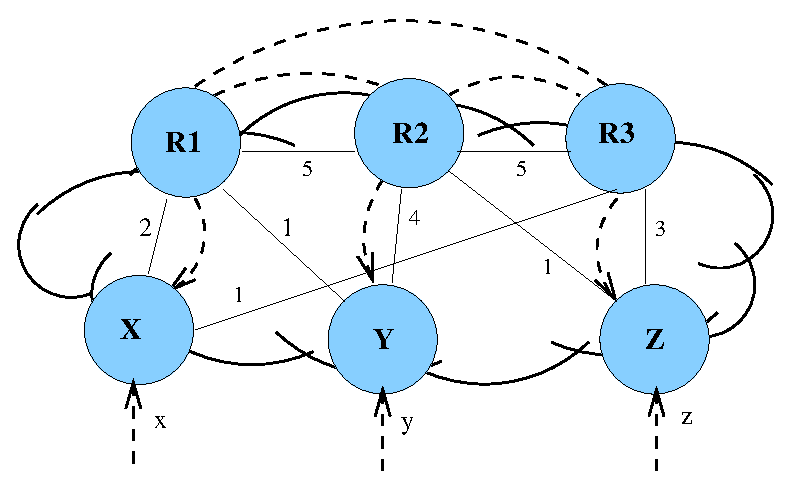
\includegraphics{rlogic/figures/sd_violation_rr_osc.eps}} 

\end{psfrags}
%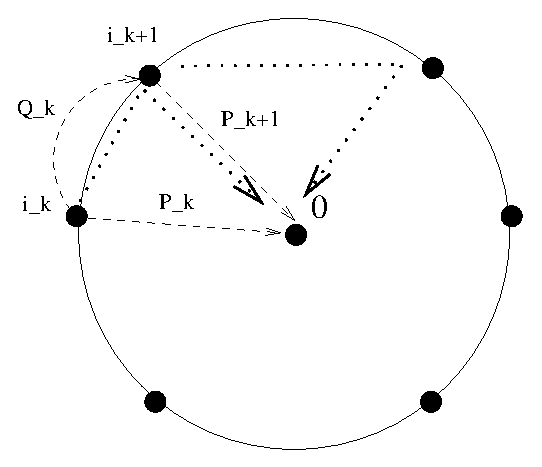
\epsfig{file=policy/figures/dw.eps,width=0.28\textwidth}
\caption[The interaction of IGP and iBGP can cause a violation of egress
  determinism.]{The interaction of IGP and iBGP can cause a violation of egress
  determinism that induces a safety violation.  This figure shows the
  instantiation of Figure~\ref{fig:abstract_sd} in BGP.  Previous work has
  also observed that violations of this type could occur~\cite{Griffin2002}
  but did not observe that these could be constructed in general by
  composing egress determinism violations.}
\label{fig:sd_violation_rr_osc}
\end{figure}


\begin{figure}
\begin{center}
\begin{psfrags}
\psfrag{R1}{{\LARGE $R_1$}}
\psfrag{R2}{{\LARGE $R_2$}}
\psfrag{X}{{\LARGE $X$}}
\psfrag{Y}{{\LARGE $Y$}}
\psfrag{Z}{{\LARGE $Z$}}
\psfrag{x}{{\Large $x$}}
\psfrag{y}{{\Large $y$}}
\psfrag{z}{{\Large $z$}}
\psfrag{l1}{{\Large $l_r$}}
\psfrag{ly}{{\Large $l_y$}}
\psfrag{lx}{{\Large $l_x$}}
\psfrag{lz}{{\Large $l_z$}}
\resizebox{0.45\textwidth}{!}{\includegraphics{rlogic/figures/det_igp.eps}}
\end{psfrags}
\end{center}
\caption[The main idea of the proof of
  Lemma~\ref{lem:det_igp}.  ]{The main idea of the proof of
  Lemma~\ref{lem:det_igp}.  
%
If $R_2$ prefers $z$ over $x$, then $l_z \leq l_x$.
%
If $R_1$ prefers $x$, given routes $x$, $y$, and $z$, then $l_y \geq
  l_r + l_x$.  If $R_2$ is on the shortest IGP path between $R_1$ and
  both $X$ and $Z$, it follows that $l_y \geq l_r + l_z$ (and, hence,
  $R_1$ would {\em not} have selected route $y$).  Thus, for $R_1$ to
  prefer route $y$ when it learns routes $x$ and $z$, its shortest path
  to either egress router $Y$ or $Z$ must not traverse $R_2$. (The links
  labeled with $l_x$, $l_y$, and $l_z$ are shown as single IGP links,
  but the argument generalizes to IGP paths.)}
\label{fig:det_igp}
\end{figure}



\begin{lemma}\label{lem:det_igp}
If an AS's iBGP topology is {\em RR-IGP-Consistent}, and every router's
selection function satisfies determinism, then every router's selection
function also satisfies egress determinism.
\end{lemma}

\begin{proof}
Suppose that there exists some router $R_1$ and routes $x$, $y$, and $z$
(not necessarily learned via eBGP at $R_1$) such that
$\lambda_{R_1}(\{x,y,z\}) = y$, but $\lambda_{R_1}(\{x,y\}) = x$.  
%
First, because $\lambda_{R_1}$ satisfies determinism, it must be the case
that (1)~$R_1$ learns $x$ via iBGP and (2)~some router $R_2$ in the iBGP
topology withdraws the eBGP-learned 
route $x$ from router $R_1$ upon learning the route $z$, thereby
preventing router $R_1$ from receiving route $x$ (if $R_1$ had learned
$x$ directly via eBGP, it would continue to select route $x$).
%
Second, $R_2$ must have selected $z$ over $x$ because it had a shorter
IGP path to the router from which it learned $z$---if $x$ had been less
desirable based on some other attribute (\eg, AS path length), then $r$
would have also selected the route $z$ upon learning it from $R_2$,
rather than selecting $y$ instead.
%
Third, because $R_1$ selects $y$ after learning $z$ from $R_2$, its IGP
path to the egress router that learned $y$ must be shorter than its IGP
path to the router that learned $z$, yet longer than its IGP path to the
router that learned $x$.   
%
This relation among distances to egresses is only possible if the
shortest path between $R_1$ and either the egress router that learned
route $x$ or $z$ does not traverse $R_2$ (\ie, the iBGP topology is not
{\em RR-IGP-Consistent}).  Figure~\ref{fig:det_igp} shows why this
relation is not possible in an iBGP topology that is {\em
RR-IGP-Consistent}.
\end{proof}

We now state the conditions for iBGP to satisfy safety using our results
involving determinism and egress determinism.  Specifically, we show
that if MED is compared across all routes (\ie, every router's selection
function satisfies determinism) and if the iBGP topology is {\em
RR-IGP-Consistent} (\ie, egress determinism is satisfied), then iBGP
satisfies safety.

\begin{figure}
\begin{center}
\begin{psfrags}
\psfrag{R1}{{\LARGE $R_1$}}
\psfrag{R2}{{\LARGE $R_2$}}
\psfrag{C1}{{\LARGE $C_1$}}
\psfrag{C2}{{\LARGE $C_2$}}
\resizebox{0.55\textwidth}{!}{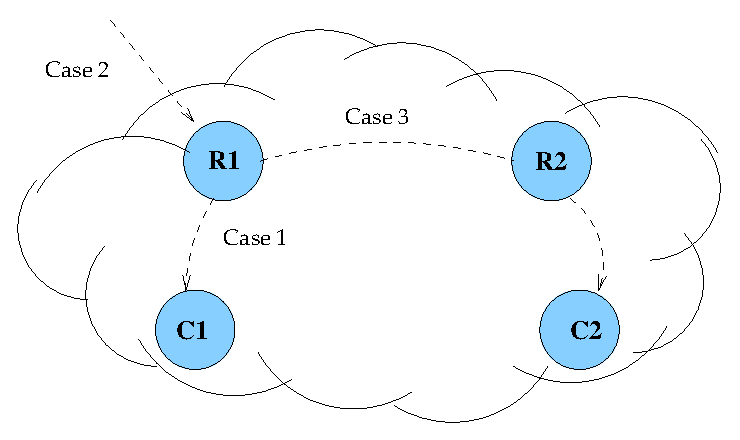
\includegraphics{rlogic/figures/always_compare.eps}} 
\end{psfrags}
\end{center}
\caption[The three cases in the proof of
  Theorem~\ref{th:always_compare}.]{The three cases in the proof of
  Theorem~\ref{th:always_compare}.}
\label{fig:always_compare}
\end{figure}



\begin{theorem}\label{th:always_compare}
If every router's selection function compares MED attribute across all
routes and the iBGP topology is {\em RR-IGP-Consistent}, then iBGP
satisfies safety.
\end{theorem}

\begin{proof}
The proof follows from Lemmas~\ref{lem:det_med} and~\ref{lem:det_igp}.
If the conditions of the theorem hold, then BGP satisfies both
determinism and egress determinism.  It remains to show that no iBGP
topology can violate safety if it satisfies both determinism and egress
determinism.  

We must show that, for any route that a router ultimately selects, other
routers in the AS will not select routes that ultimately causes the
original router to change the route it selects.  For simplicity, we will
consider an iBGP route reflector hierarchy with one level.  The argument
can be extended to a multiple-level hierarchy, and to a network with
multiple top-level routers or multiple clients per route reflector,
without loss of generality.  Consider the possible propagation of BGP
routes between routers $C_1$ and $C_2$ and their route reflectors $R_1$
and $R_2$, as shown in Figure~\ref{fig:always_compare}.  Suppose $C_1$
and $C_2$ initially select routes via eBGP; each will readvertise these
routes to $R_1$ and $R_2$.  Then, there are three cases:

\begin{enumerate}
\itemsep=-1pt
\item {\em $R_1$ prefers the route through its client $C_1$.}
In this case, $R_1$'s selection of the route through $C_1$ will
obviously not cause either $R_1$ or $C_1$ to switch paths.  
%
\item {\em $R_1$ prefers its own eBGP-learned route (analogously for
$R_2$).}  In this case, $C_1$ learns a route via $R_1$. If it
continues to prefer its own route, neither router will select a new
route. If, on the other hand, it prefers the route through $R_1$, then
it will withdraw its eBGP-learned route from $R_1$.  However, since
$\lambda_{R_1}$ satisfies determinism, $R_1$ will continue to select its
own eBGP-learned route when it receives this withdrawal.
%
\item {\em $R_1$ prefers a route via $R_2$ or $C_2$ (analogously for
$R_2$).}  A similar argument can be used to show that
neither $R_1$ nor $C_1$ will select a new route once $R_1$ selects a
route via $C_1$.  For the third case, we must also show that $R_1$'s
withdrawal of either its own route or the route via $C_1$ from $R_2$
will cause neither $R_2$ nor $C_2$ to change routes.  Since $R_1$
prefers a route via $R_2$ then $R_2$ selected its own route
or the route via $C_2$; egress determinism guarantees that $R_1$'s
withdrawal will not cause either $C_2$ or $R_2$ to change its route
selection.
\end{enumerate}
\end{proof}

Our definitions have allowed us to derive sufficient
conditions on safety that are significantly weaker (and therefore, the
result is stronger) than in
previous work~\cite{Griffin2000}.  In particular, {\em our results show
that assuming that the relationships between route reflectors and their
clients are acyclic is unnecessary} (although a cyclic topology may make
an oscillation more likely if egress determinism is
violated).  It turns out that the only way for a cyclic iBGP topology
to cause oscillations would be for either the iBGP topology to not be
{\em RR-IGP-Consistent} or for some IGP edges to have
negative edge weights.

\begin{figure}
\centering
\begin{psfrags}
%
\psfrag{x}{{\LARGE $x$}}
\psfrag{y}{{\LARGE$y$}}
\psfrag{z}{{\LARGE $z$}}
\psfrag{X}{{\LARGE $X$}}
\psfrag{Y}{{\LARGE $Y$}}
\psfrag{Z}{{\LARGE $Z$}}
\psfrag{R1}{{\LARGE $R_1$}}
\psfrag{R2}{{\LARGE $R_2$}}
\psfrag{R3}{{\LARGE $R_3$}}
\psfrag{l1}{{\LARGE $l_1$}}
\psfrag{l2}{{\LARGE $l_2$}}
\psfrag{l3}{{\LARGE $l_3$}}
\psfrag{l4}{{\LARGE $l_4$}}
\psfrag{l5}{{\LARGE $l_5$}}
\psfrag{l6}{{\LARGE $l_6$}}
%
%\hspace{-0.7in}
\resizebox{0.7\textwidth}{!}{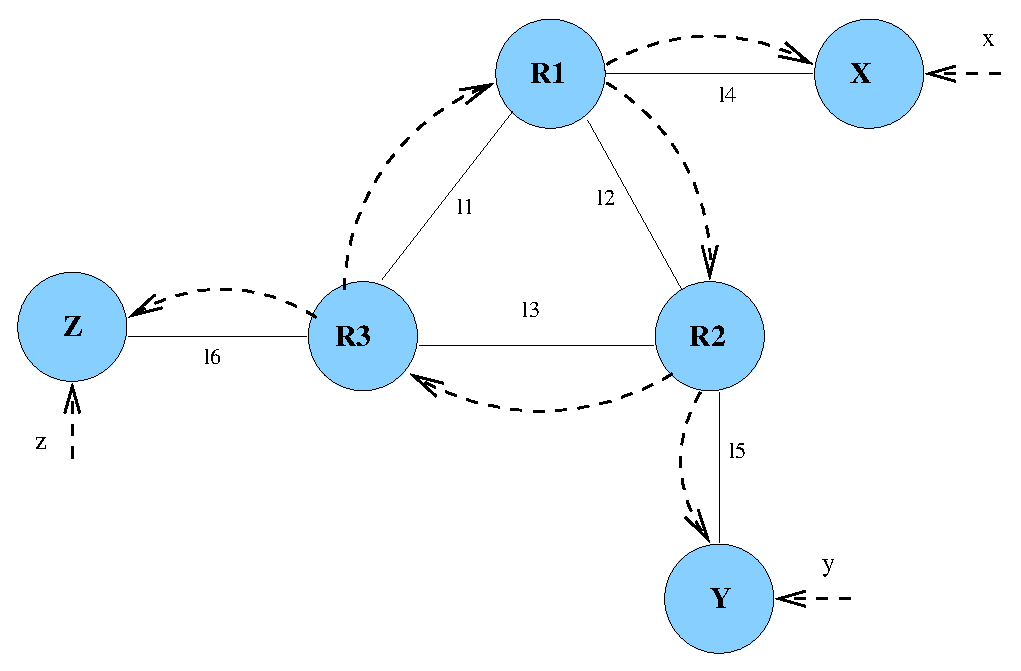
\includegraphics{rlogic/figures/ibgp_cycle.eps}} 

\end{psfrags}
%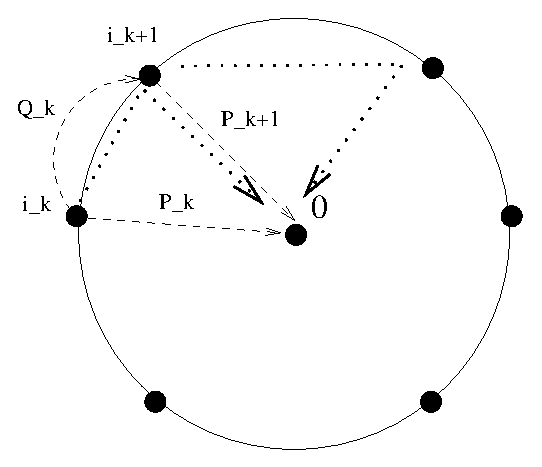
\epsfig{file=policy/figures/dw.eps,width=0.28\textwidth}
\caption[When iBGP satisfies egress determinism,
  a cyclic iBGP topology typically do not cause safety violations.]{When iBGP
  violates safety but satisfies egress determinism, the only way a
  cyclic iBGP topology can 
  violate safety is if the IGP allows negative edge weights.  This
  example shows an iBGP hierarchy that includes only six routers, but it
  generalizes: $R_i$ could be any cyclic relationship at the top of the
  hierarchy, $X$ could be a path through a sequence of iBGP sessions to
  the egress router $X$ (\eg, a sequence of route reflector-client
  sessions) and $l_4$ could be the cost of that path, and so forth.}
\label{fig:ibgp_cycle}
\end{figure}



To understand why cycles in the iBGP hierarchy do not cause problems if
the topology is {\em 
RR-IGP-Consistent}, see Figure~\ref{fig:ibgp_cycle}.  In this example,
if egress determinism is satisfied, then the only case where an
oscillation might result is where $R_1$ prefers route $y$ over route
$x$, $R_2$ prefers route $z$ over $y$, and $R_3$ prefers $x$ over $z$.
All other cases where oscillation might occur (\ie, those caused by
violations of egress determinism) require some shortest IGP path between
a router and another egress to not traverse that router's route reflector.
For safety to be violated in this example, routes $x$, $y$, and $z$ must
all have equal local preference, AS path length, origin type and MED
(otherwise, all routers would select the most preferable route or
routes).  Presuming that all routes are equally good up to the step in
route selection involving the IGP tiebreak, then the only way for such a
situation to occur is if the following inequalities were satisfied:
\begin{eqnarray*}
l_1 + l_4 & < & l_6 \\
l_2 + l_5 & < & l_4 \\
l_3 + l_6 & < & l_5 
\end{eqnarray*}
which implies that $l_1 + l_2 + l_3 < 0$, or that some IGP edge weights
must be negative.

Theorem~\ref{th:always_compare} is significant because
the conditions on the iBGP topology that are required to guarantee
safety are identical those for guaranteeing route validity, as stated in
Theorem~\ref{th:rr_safe}.  Furthermore, because there are now known
techniques for {\em generating} these
configurations~\cite{Vutukuru2005}, our results are prescriptive, since
this technique that was designed to generate iBGP topologies that
guarantee route validity also happens to generate topologies that
guarantee safety.

This section has described safety violations that result from
protocol interactions {\em within a single AS}.  However, safety is a somewhat
unique property because it inherently depends on how different ASes are
allowed to rank candidate routes to a destination (\ie,
Observation~\ref{obs:composable} is not satisfied).  Whereas, in iBGP, a
router's rankings are constrained by the underlying IGP
topology, in eBGP, an AS's rankings can be arbitrary.
Verifying a property that involves analyzing the interactions
between the configurations of multiple ASes is challenging:
because these ASes compete with one another, no single AS has knowledge 
of the configurations of other ASes.  Chapter~\ref{chap:policy} explores
how safety can be guaranteed {\em across multiple ASes} without
requiring each AS to expose its configurations to other ASes.


\section{Summary}

Detecting problems in Internet routing requires a precise
specification of correct behavior and a framework for reasoning about
whether that specification is satisfied.  In this chapter, we presented
a three-part correctness specification: route validity, path visibility,
and safety. We explained why each of these properties is important for the
fundamental operation of Internet routing and reasoned about how these
properties may be satisfied or violated in the context of BGP.

In the subsequent chapters of this dissertation, we will use the
specification constraints to guide the operations and design of correct
Internet routing.  In Chapter~\ref{chap:rcc}, we will explore how static
configuration analysis can be used to guarantee that two of these
properties---route validity and path
visibility---hold. 
Theorems~\ref{th:mesh}--\ref{thm:vis}
%, \ref{th:rr_safe},
%\ref{th:mesh_visibility}
%, and~\ref{thm:vis} 
suggest invariants on
configuration that could be verified by detecting when the configuration
violates certain invariants, and both Theorem~\ref{th:always_compare}
and the discussion at the end of
Section~\ref{sec:mesh}
suggest possible protocol modifications.  In
Chapter~\ref{chap:sandbox}, we will exploit the fact that, when the
routing protocol satisfies certain aspects of this specification
(specifically, path visibility, safety, and, in some cases,
determinism), we can design algorithms that efficiently predict the
routes that each router in an AS will ultimately select.
Chapter~\ref{chap:policy} tackles the problem of guaranteeing safety in
the context of eBGP, which is challenging since it inherently involves
dependencies between the policies of multiple independent (and often
competing) ASes.
%Chapter~\ref{chap:beyond} explores how both analysis of
%routing protocol dynamics and modifications to the routing architecture
%itself can complement static configuration analysis.





\qchapter{\textit{Things could be worse. \\  Suppose your errors were
    counted and published every day, \\ like those of a baseball player.}
    \vskip 0.1em  - Unknown}{\rccns: Detecting BGP Configuration Faults with Static
  Analysis}\label{chap:rcc} 

%\section{Introduction}

\cs{T}his chapter describes the design, implementation, and evaluation of
\textbf{\rccns},
the router configuration checker, a tool
that uses static analysis to detect faults in Border Gateway Protocol
(BGP) 
configuration.  
By finding faults over a
distributed set of router configurations, \rcc enables network
operators to test and debug configurations before deploying them in an
operational network. This approach improves on the status quo of
``stimulus-response'' debugging where operators need to run
configurations in an operational network before finding faults.

As described in Chapter~\ref{chap:related} (Section~\ref{sec:conf}),
network operators use router configurations to provide reachability,
express routing policy (\eg, transit and peering
relationships~\cite{Norton2000}, inbound and outbound
routes~\cite{Beijnum2002}, etc.), configure primary and backup
links~\cite{Gao2001b}, and perform traffic engineering across multiple
links~\cite{Feamster2004}.  The complex process of configuring routers
is exacerbated by the number of lines of code, by configuration being
distributed across the routers in the network, by the absence of useful
high-level primitives in today's configuration languages, by the
diversity in vendor-specific configuration languages, and by the number
of ways in which the same high-level functionality can be expressed in a
configuration language.  

Router configuration gives network operators the flexibility to control
traffic and implement complex business relationships, but its complexity
also means that router configurations are prone to
faults~\cite{Beijnum2002,Mahajan2002}.  Configuration faults include
invalid routes (including hijacked and leaked routes); contract
violations~\cite{Feamster2004b}; unstable routes~\cite{labovitz:ton01};
routing loops~\cite{Dube99,Feamster2003b}; and persistently oscillating
routes~\cite{Basu2002,Griffin99,Varadhan2000}.
%Section~\ref{s:nanogproblems} discusses the problems observed in
%operational networks in detail.  
As summarized in
Table~\ref{tab:empirical_results} (Section~\ref{sec:rcc_related}), BGP
configuration faults can seriously affect end-to-end Internet
connectivity, leading to lost packets, forwarding loops, and unintended
paths between hosts or ASes.  


\begin{figure}[t]
\begin{center}
%\resizebox{0.8\columnwidth}{!}{\includegraphics*[viewport=100 200 500 650]{rcc/figures/nanog_table.pdf}}
\centering\epsfig{file=rcc/figures/nanog_table.eps, angle=270, width=\linewidth}
\end{center}
\caption{Number of threads discussing routing
  faults on the NANOG mailing list.
}
\label{tab:nanogerrors}
\end{figure}


%% Chapter~\ref{chap:related} (Section~\ref{sec:configuration})
%% describes how BGP's configuration affects which routes are originated
%% and propagated, how routes are modified as they propagate, which route
%% each router selects from multiple options, and how routes propagate
%% between routers.  
To understand the extent to which this complex configuration is
responsible for the types of failures that occur in practice, we studied
the archives of the North American Network Operators Group (NANOG)
mailing list, where network operators report operational problems,
discuss operational issues, etc.~\cite{nanog-list}.  Because the list
has received about 75,000 emails over the course of ten years, we first
clustered the emails by thread and pruned threads based on a list of
about fifteen keywords (\eg, ``BGP'', ``issue'', ``loop'', ``problem'',
``outage'').  We then reviewed these threads and classified each of them
into one or more of the categories shown in
Figure~\ref{tab:nanogerrors}.  This informal study shows some clear
trends.  First, many routing problems are caused by configuration
faults.  Second, the same types of problems continually appear.  Third,
BGP configuration problems continually perplex even experienced network
operators.  A tool like \rcc that can {\em proactively} detect
configuration faults will 
clearly benefit network operators.



Remarkably, static configuration analysis
can detect many of these configuration faults before the faulty
configuration is ever deployed on a live network.

Detecting BGP configuration faults poses several challenges beyond
simply defining a correctness specification.
%
First, a high-level correctness specification, such as the one defined
in Chapter~\ref{chap:rlogic}, must be used to derive a set of
constraints that can be tested against the actual configuration.
%
Second, BGP configuration is distributed---analyzing routing
configuration requires both synthesizing distributed configuration
fragments and representing the configuration in a form that makes it
easy to test constraints.
%
This chapter tackles these challenges and makes the following
two contributions:


\begin{enumerate}
\itemsep=-1pt
\item We present the design and implementation of {\bf \rccns}.
\rcc focuses on detecting faults that have the potential to cause {\em
  persistent} routing failures.  \rcc is not concerned with
correctness during convergence (since any distributed protocol will
have transient inconsistencies during convergence).  \rccns's goal is
to detect problems that may exist in the steady state, even when the
protocol converges to some stable outcome.

\item We use \rcc to explore the extent of real-world BGP
configuration faults; this chapter presents the first published analysis
of BGP configuration faults in real-world ISPs.  
We have analyzed real-world,
deployed configurations from 17 different ASes and detected more than
1,000 BGP configuration faults that had previously gone undetected by
operators.  These faults ranged from simple ``single router'' faults
(\eg, undefined variables) to complex, {\em network-wide} faults
involving interactions between multiple routers.  
To date, \rcc has been downloaded by over seventy network operators.
\end{enumerate}

\rcc is intended to be used {\em before} configurations are
deployed, but we also used \rcc to study the deployed configurations of live,
operational networks.  In these networks, \rcc discovered many
faults that could potentially cause failures.  These include: (1) faults
that could have caused network partitions due to errors in how external
BGP information was being propagated to routers inside an AS, (2) faults
that caused invalid routes to propagate inside an AS, and (3) faults in
policy expression that caused routers to advertise routes (and hence
potentially forward packets) in a manner inconsistent with the AS's
desired policies.
%
Our findings indicate that configuration faults that can
cause serious failures are often not immediately apparent (\ie, the
failure that results 
from a configuration fault may only be triggered by a specific failure
scenario or sequence of route advertisements).  If \rcc were used before
BGP configuration was deployed, we expect that it would be able to
detect faults that immediately caused routing failures as well.

Our analysis of real-world configurations suggests that most
configuration faults stem from three main causes.  First, the mechanisms
for propagating routes within a network are overly complex.  The main
techniques used to propagate routes scalably within a network (\eg,
``route reflection with clusters'') are easily misconfigured.  Second,
many configuration faults arise because configuration is distributed
across routers: even simple policy specifications require configuration
fragments on multiple routers in a network.  Third, configuring policy
often involves low-level mechanisms (\eg, ``route maps'', ``community
lists'', etc.)  that should be hidden from network operators.

The rest of this chapter proceeds as follows.
Section~\ref{sec:rcc_overview} describes the design of \rccns.
Sections~\ref{sec:visibility} and~\ref{sec:validity} highlight some of \rccns's
path visibility and route validity tests.
Section~\ref{sec:implementation} describes implementation details.
Section~\ref{sec:evaluation} presents configuration faults that \rcc
discovered in 17 operational networks.  Section~\ref{sec:rcc_lessons}
summarizes the take-away lessons from this study, and
Section~\ref{s:rcc_concl} concludes.

%\section{Motivation}
\label{s:background}
\label{s:nanogproblems}




\begin{figure}[t]
\begin{center}
\centering\epsfig{file=rcc/figures/nanog_table.eps, angle=270, width=\linewidth}
\end{center}
\caption{Number of threads discussing routing
  faults on the NANOG mailing list.
}
\label{tab:nanogerrors}
\end{figure}


Chapter~\ref{chap:related} (Section~\ref{sec:configuration})
describes how BGP's configuration affects which routes are originated
and propagated, how routes are modified as they propagate, which route
each router selects from multiple options, and how routes propagate
between routers.  
To understand the extent to which this complex configuration is
responsible for the types of failures that occur in practice, we studied
the archives of the North American Network Operators Group (NANOG)
mailing list, where network operators report operational problems,
discuss operational issues, etc.~\cite{nanog-list}.  Because the list
has received about 75,000 emails over the course of ten years, we first
clustered the emails by thread and pruned threads based on a list of
about fifteen keywords (\eg, ``BGP'', ``issue'', ``loop'', ``problem'',
``outage'').  We then reviewed these threads and classified each of them
into one or more of the categories shown in
Figure~\ref{tab:nanogerrors}.

This informal study shows some clear trends.  First, many routing
problems are caused by configuration faults.  Second, the same
types of problems continually appear.  Third, BGP
configuration problems continually perplex even experienced network
operators.  A tool that can detect configuration faults will clearly
benefit network operators.

\input{rcc/overview}
\input{rcc/signaling}
\section{Route Validity Faults}\label{sec:validity}

BGP should satisfy {\em route validity}, as defined formally in
Chapter~\ref{chap:rlogic} (Definition~\ref{defn:rv}).
%BGP configuration affects which routes each router accepts, selects, and
%readvertises.  
Table~\ref{tab:rcc_tests} summarizes the route validity faults that \rcc
checks.  The biggest challenge for checking route validity is
that the definition says that the routes the routers in an AS select
should induce only policy-conformant paths (see
Definition~\ref{defn:pcp}), but \rcc operates without a specification of
the intended policy.  This section focuses on \rccns's approach to
detecting potential policy-related problems.

Requiring operators to provide a high-level policy specification would
require designing a specification language and convincing operators to
use it, and it provides no guarantees that the results would be more
accurate, since errors may be introduced into the specification itself.
Instead, \rcc forms {\em beliefs} about a network operator's intended
policy in two ways: (1)~assuming that intended policies conform to best
common practice and (2)~analyzing the configuration for common patterns
and looking for deviations from those patterns.  (The idea of forming
beliefs about intended protocol behavior is inspired from similar ideas
in systems~\cite{Engler01}.)  \rcc then finds cases
where the configuration appears to violate these beliefs.  It is
noteworthy that, even in the absence of a policy specification, this
technique detects many meaningful configuration faults and generates few
false positives.

%% An AS's customers will sometimes advertise smaller prefixes to its upstream
%% AS to load balance its inbound traffic, but it will tag those prefixes
%% with an instruction to its upstream to not readvertise these
%% prefixes~\cite{rfc1997}.  The export policies on an AS's routers should
%% always ensure that such a route is not readvertised to any neighbors.
%% Network operators also control the export of routes between
%% their peers and providers.  Static analysis can check this property by
%% analyzing the configuration files to verify that every eBGP session has
%% a filter that matches routes that have this instruction and prevents
%% them from being readvertised to other ASes.

\subsection{Violations of Best Common Practice}

We can derive some notions of high-level policy from our knowledge of
best common practice (\ie, the manner in which many ASes
tend to configure their 
networks).  In particular, \rcc looks for two violations of best common
practice: (1)~advertising a route from one ``peer'' to another (\ie, a
violation of the common business practices defined in
Table~\ref{tab:business} (Section~\ref{sec:semantics}); and (2)~not
advertising routes in a consistent manner at all peering
points~\cite{Feamster2004b}.  In this section, we explain both of these
practices in more detail.

A route that an AS learns from one of its ``peers'' should not be
readvertised to another peer.  Checking this condition requires
determining how a route propagates through an AS.
Figure~\ref{fig:policy_closure} illustrates how \rcc performs this
check.  Suppose that \rcc is analyzing the configuration from AS $X$ and
needs to determine that no routes learned from AS $B$ are exported to
AS $A$.  First, \rcc determines all routes that AS $X$ exports to AS $A$,
typically a set of routes that satisfy certain constraints on their
attributes. For example, router $R_1$ may export to AS $A$ only routes
that are ``tagged'' with the label ``$1000$''.  As described in
Section~\ref{sec:conf}, ASes often assign such ``community'' labels to a
route to
control how other routers rank or filter it. \rcc then checks the {\em
import} policies for all sessions to AS $B$, ensuring that no import
policy will set route attributes on any incoming route that would place
it in the set of routes that would be exported to AS $A$.  To perform
this check, \rcc must know which of an AS's neighboring ASes are peers;
thus, this check requires this additional input from the network
operator.

Additionally, an AS should advertise routes with equally good attributes
to each peer at every peering point.  An AS should not advertise routes
with inconsistent attributes, since doing so may prevent its peer from
implementing ``hot potato'' routing:
If ASes $1$ and $2$ are
peers, then the export policies of the routers in AS $1$ should export
routes to AS $2$ that have equal AS path length and MED values.  If not,
router $X$ could be forced to send traffic to AS $1$ via router $Y$
(``cold potato'' routing).
This behavior typically violates peering
agreements.  Recent work has observed that this type of inconsistent
route advertisement sometimes occurs in practice~\cite{Feamster2004b}.

An AS's policies may violate this best common practice for two reasons.
First, an AS may apply different export policies at different routers to
the same peer.  Checking for consistent export involves comparing export
policies on each router that has an eBGP session with a particular peer.
Static configuration analysis is useful because it can efficiently
compare policies on 
many different routers.  In practice, this comparison is not
straightforward because differences in policy definitions are difficult
to detect by direct inspection of the distributed router configurations.
\rcc facilitates comparing export policies across sets of routers by
normalizing all of the export policies for an AS, as described in
Table~\ref{tab:if} (Section~\ref{sec:rcc_overview}).  Second, an iBGP
signaling partition can 
create inconsistent export policies because routes with equally good
attributes may not propagate to all peering routes.  For example,
consider Figure~\ref{f:ibgp_vis_violation} again.  If routers $W$ and
$Z$ both learn routes to some destination $d$, then route $W$ may learn
a ``better'' route to $d$, but routers $Y$ and $Z$ will continue to
select the less attractive route.  If routers $X$ and $Y$ readvertise
their routes to a peer, then the routes advertised by $X$ and $Y$ will
not be equally good.  Thus, \rcc also checks whether routers that
advertise routes to the same peer are in the same iBGP signaling
partition (as described in Section~\ref{sec:visibility}, \rcc checks for
all iBGP signaling partitions, but ones that cause inconsistent
advertisement are particularly serious).

\subsection{Configuration Anomalies}

\begin{figure}
\begin{center}
\begin{psfrags}
\psfrag{AS A}{AS $A$}
\psfrag{AS B}{AS $B$}
\psfrag{AS X}{{\LARGE AS $X$}}
\psfrag{R1}{$R_1$}
\resizebox{0.85\textwidth}{!}{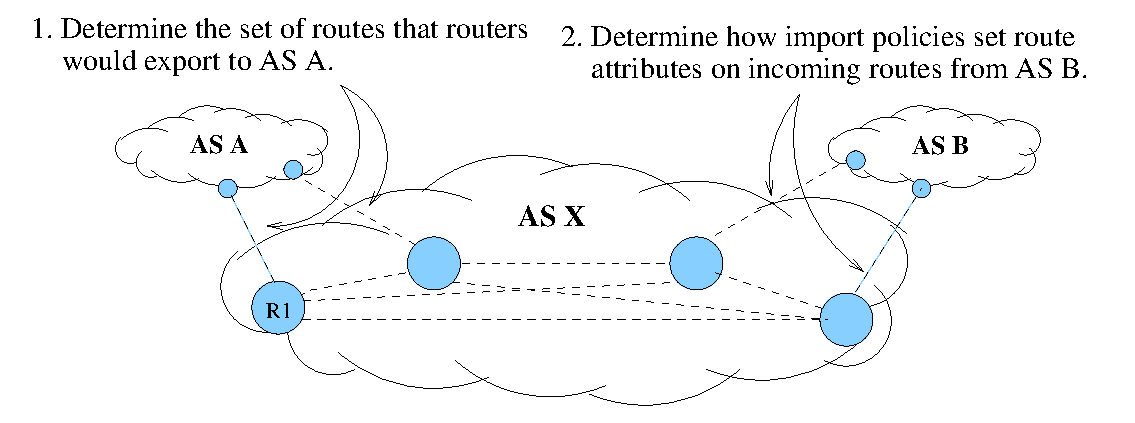
\includegraphics{rcc/figures/policy_closure.eps}}
\end{psfrags}
\end{center}
\caption{How \rcc computes route propagation.}
\label{fig:policy_closure}
\end{figure}

When the configurations for sessions at different routers to a
neighboring AS are the same except at one or two routers, the deviations
are likely to be mistakes.  This test relies on the belief that, if an
AS exchanges routes with a neighboring AS on many sessions and most of
those sessions have identical policies, then the sessions with slightly
different policies may be misconfigurations.  Of course, this test could
result in many false positives because there are legitimate reasons for
having slightly different import policies on sessions to the same
neighboring AS (\eg, outbound traffic engineering), but it does provide
a useful sanity check.

%% that all
%% routes received from a peer look equally good up to the IGP tiebreak
%% step, thus allowing it to use nearest exit (``hot potato'') routing with
%% its peers.  Of course, an AS cannot ensure that it receives AS paths of
%% equal length at all peering points with its peer, but it can take
%% precautions such as resetting the MED value on import and ensuring that
%% the local preference value is the same everywhere.  


\input{rcc/implementation}
\input{rcc/evaluation}
\section{Take-away Lessons}\label{sec:rcc_lessons}


In recent years, much work has been done to understand BGP's
behavior, and much has been written about the wide range of problems it
has.  Some argue that BGP has outlived its purpose and should be
replaced; others argue that faults arise
because today's configuration languages are not
well-designed.  We believe that our evaluation of faults in
today's BGP configuration provides a better understanding of the
types of errors that appear in today's BGP configuration and the
problems in today's configuration languages.  
%
%Our evaluation of real-world BGP configuration from operational networks
%suggests several higher-level lessons about the nature of today's
%configuration process.  
We now briefly explore how our findings may help inform the design
of Internet routing systems in the future.

First, operational networks---even large, well-known, and well-managed
ones---have faults.  Even the most competent of operators find it
difficult to manage BGP configuration.  In particular, iBGP is
misconfigured often.  In fact, in the absence of a guideline such as
Theorem~\ref{thm:vis}, it is hard for a network operator to know what
properties the iBGP signaling graph should have.  Ideally, network
operators should be able to configure an AS without having to worry
about whether these types of constraints are satisfied in the first
place; in other words, a network operator should not be allowed to
express a configuration that violate properties such as path visibility
and route validity.  In Chapter~\ref{chap:concl}
(Section~\ref{sec:rcp}), we discuss a system for disseminating BGP
routes within an AS called the Routing Control Platform
(RCP)~\cite{caesar2004,feamster:fdna2004}, which could explicitly
enforce properties such as route validity and path visibility.

%
Second, we found that route filters are poorly maintained.  Routes that
should never be seen on the global Internet (\eg, routes for private
addresses) are rarely filtered, and the filters that are used are often
misconfigured and outdated.  We can make significant strides towards
fixing these types of problems simply by changing the default behavior
of router filters.  For example, because private address space (\ie, as
specified in RFC 3330~\cite{rfc3330}) should not be advertised on the
global Internet, routers could, by default, prevent routes for this
address space from leaking across AS boundaries.  Of course, network
operators who required routes for this address space to be advertised
across AS boundaries (\eg, in cases where a single administrative domain
comprises multiple ASes) could configure that behavior as an {\em
exception}, but the default behavior would reduce the likelihood of
erroneous route leaks.

%
Third, the majority of the configuration faults that \rcc detected
resulted from the fact that an AS's configuration is distributed across
its routers.  Maintaining network-wide policy consistency appears to be
difficult; invariably, in most ASes there are routers whose
configuration appears to contradict the AS's desired policy.  A routing
architecture or configuration management system that enabled an operator
to configure the network from a centralized location with a high-level
language would likely prevent many serious faults.

%
Finally, although operators use tools that automate some aspects of
configuration, these tools are not a panacea.  In fact, we found cases
where the incorrect use of these tools {\em caused} configuration
faults.  This observation suggests that static configuration
analysis will play an important role in the configuration
workflow, regardless of future improvements in configuration languages
or routing architectures.  As long as the routing protocol offers
flexible configuration, the potential for incorrect behavior exists.
Our work has demonstrated that detecting incorrect behavior {\em
proactively} using static configuration analysis is not only
surprisingly effective, but it is also necessary for detecting faulty
configurations before they introduce erroneous behavior on a live
network. 



\section{Summary}
\label{s:rcc_concl}


Despite the fact that BGP is almost 10 years old, operators continually make
the same mistakes as they did during BGP's infancy.   Our work takes a
step towards improving this state of 
affairs by making the following contributions:
%\vspace*{-0.05in}
\begin{itemize}
\itemsep=-1pt
%\item We define a high-level correctness specification for BGP and
%  map that specification to conditions that can be tested with static
%  analysis.
\item We use the correctness specification from Chapter~\ref{chap:rlogic}
  to design and implement 
  \rccns, a static analysis tool that detects faults by analyzing the
  BGP configuration across a single AS.  With \rccns, network operators
  can find many faults {\em before} deploying configurations in
  an operational network.  \rcc has been downloaded by over seventy network
  operators.
\item We use \rcc to explore the extent of real-world BGP
      misconfigurations.  We have analyzed
      real-world, deployed configurations from 17 different ASes and
      detected more than 1,000 BGP configuration faults that had
      previously gone undetected by operators.
\end{itemize}



%framework to the design and implementation of \rccns, a tool that uses
%static analysis to verify BGP configuration correctness.  Our tool has
%helped operators debug real-world BGP configuration.  Third, we
%present our findings on BGP configuration errors and anomalies from
%static analysis of real-world BGP configurations.  This paper is the
%first to explore BGP configuration errors using analysis of real-world
%BGP configuration files.  Finally, we suggest concrete ways to improve
%BGP's correctness, distinguishing problems that should be fixed with
%protocol modifications from those that should be fixed with a better
%configuration language.

In light of our findings, we suggest two ways to make interdomain
routing less prone to configuration faults.  First, protocol
improvements, particularly in intra-AS route dissemination, could avert
many BGP configuration faults.  The current approach to scaling iBGP
should be replaced.  Route reflection serves a single, relatively simple
purpose, but it is the source of many faults, many of which cannot be
checked with static analysis of BGP configuration
alone~\cite{Griffin2002}.  The protocol that disseminates BGP routes
within an AS should enforce path visibility and route validity; the
Routing Control Platform offers one possible solution.

Second, BGP should be configured with a centralized, higher-level
specification language.  Today's BGP configuration languages enable an
operator to specify router-level {\em mechanisms} that implement
high-level policy, but the distributed, low-level nature of the
configuration languages introduces complexity, obscurity, and
opportunities for misconfiguration rather than design flexibility or
expressiveness.  For example, \rcc detects many faults in implementation
of some high-level policies in low-level configuration; these faults
arise because there are many ways to implement the same high-level
policy, and the low-level configuration is unintuitive.  Ideally, a
network operator would never touch low-level mechanisms (\eg, the
community attribute) in the common case.  Rather than configuring
routers with a low-level language, an operator should configure the {\em
network} using a language that directly reflects high-level
policies.



%, and this specification could be ``compiled'' into
%configuration statements that implement the policies.
% (Such a specification would also be much easier to analyze
%with a tool like \rccns.)



%XXX FUTURE WORK: IGP/iBGP...

%% The hard stuff, like iBGP, isn't going to get better.  Same with things
%% like MED osc.  For these, we need protocol changes.  This is part of our
%% ongoing work (\eg, route servers to impose a total ordering, scrap iBGP
%% to avoid partitions, guarantee consistent export, etc.)

%% Same thing with safety.  It's fundamental to the protocol (Arrow's
%% impossibility thm), and protocol changes must happen to solve this
%% problem correctly.

%% For other stuff that people mess up, we need better interfaces.  These
%% interfaces should reflect that there are only a handful of tasks that
%% operators need to perform.


% Herb Caen:  "The clock doesn't matter in baseball. Time stands still or moves backwards. Theoretically, one game could go on forever. Some seem to."

%"Slow it down to stay ahead of it to stay on top of it." -Tony LaRussa

%"There are three types of baseball players: those who make it happen,
%those who watch it happen, and those who wonder what happens." - Tommy Lasorda

%Abbott: Now, on the St. Louis team we have Who's on first, What's on
%second, I Don't Know is on third. Costello: That's what I want to find
%out.

% I say Who's on first, What's on second, I Don't Know's on third.
%- Lou Costello 


\qchapter{\textit{There are three types of baseball players: those who
make it happen, \\ those who watch it happen, and those who wonder what
happens.} \vskip 0.1em - Tommy Lasorda}{Predicting BGP Routes with
Static Analysis}\label{chap:sandbox}

%% \cs{T}he complexity of Internet routing configuration and protocol
%% dynamics mandates a framework for understanding and manipulating
%% Internet routing at a level of abstraction that facilitates reasoning
%% about whether or not the protocol is behaving ``correctly''.  Naturally,
%% the first step in this process is defining what it means for a routing
%% protocol to operate correctly in the first place.  Specifying
%% correctness is not easy, because it requires distilling a high-level
%% description of how the routing protocol should behave from the myriad
%% technical minutia of the operation of the protocol.

\cs{T}he flexibility offered by Internet routing configuration
allows the protocol to scale well and enables operators to express a wide
variety of policies, but it increases the complexity of the system.  This
complexity makes it difficult to reason about the behavior of Internet
routing, leading to {\em ad hoc} fixes to observed problems that
ultimately only worsen this complexity.  Today, network operators (who
continually tweak routing configuration) and protocol designers
(who repeatedly propose ``point'' solutions to various problems) have
no way of reasoning about whether their modifications to Internet
routing will
operate as intended.  Worse yet, operators and designers do not even
have a {\em specification} of properties that Internet routing should
satisfy.  This chapter seeks to remedy this situation by specifying
correctness properties
that any routing protocol should satisfy.

We introduce three properties to
classify the behavior of a routing protocol.  We briefly describe
these properties below and explain why they are critical for
correct routing.

\begin{enumerate}
\itemsep=-1pt
\item {\em Route validity} states that if a router has a route to a
destination, then a usable path corresponding to that route exists in
the underlying topology.  If route
validity is violated, then end users could experience a failure of
end-to-end connectivity, because routers could forward packets along
non-existent paths.
%; for example, routers may ``blackhole'' traffic,
%or the traffic may get caught in a loop and may never reach the
%destination.
\item {\em Path visibility} states that if there is a usable path
between two nodes, then the routing protocol will propagate information
about that path.  A failure of path visibility could disrupt
end-to-end communication by preventing two connected nodes from learning
routes between one another.
\item {\em Safety} states that the routing protocol converges to a
stable route assignment, regardless of the order in which routing
messages are exchanged.  A routing protocol that violates safety will
induce persistent route oscillations, causing routing changes that
are unrelated to changes in topology or policy.
\end{enumerate}
\noindent
This chapter defines and investigates these properties and
demonstrates how they can 
deepen our understanding of network routing.
This correctness specification addresses {\em static} properties of
network routing, {\em not} dynamic behavior (\ie, its response to
changing inputs, convergence time, etc.). Internet routing, like any
distributed protocol, may experience periods of transient incorrectness
in response to changing inputs, but we are concerned with persistent
misbehavior.

Chapter~\ref{chap:rcc} presents an approach to detect when two
of these properties (route validity and path visibility) are violated.
Chapter~\ref{chap:sandbox} exploits
these properties to predict which
of many possible routes each router in the network will select.
Chapter~\ref{chap:policy} deals with the 
challenges of guaranteeing safety, an inherently global property.
%Chapter~\ref{chap:beyond} discusses how both dynamic analysis and
%routing protocol improvements can help guarantee these properties.

%Previous work in wide-area protocol design
%has focused on specific modifications to BGP that fix a particular
%problem but often spur unintended negative side effects.  Furthermore,
%designers of new wide-area routing protocols require a mechanism that
%enables them to reason about the circumstances under which the protocol
%will behave ``correctly''.  To help reason about modifications to
%existing routing protocols and to aid in the sound design of new ones in
%the future, we propose that routing protocols be classified in terms of
%specific high-level properties.

After we introduce some basic terminology in
Section~\ref{sec:definitions}, we motivate and describe the correctness
properties.  Sections~\ref{sec:validity_def},
\ref{sec:visibility_def},~and
\ref{sec:safety_def} 
describe route validity, path visibility, and safety, respectively, and
explain how various aspects of the operation and configuration
of the Internet's routing protocols can cause each of these to be
violated in practice.   

%%%
%%% setup.tex
%%%


\section{Modeling Constraints and Algorithm Overview}
\label{sec:setup}
%%%
%%% Introduction
%%%
In this section, we impose three constraints that the routing system
must satisfy to enable efficient and accurate route prediction.  

Next, we describe how these constraints enable us to decompose the
algorithm into three stages---applying the import policy to eBGP-learned
routes, selecting the best BGP route at each router, and computing the
forwarding path.  The algorithm takes as input the router configuration
and a static snapshot of the routes learned via eBGP and outputs the
route that each router in the AS selects, for each destination.  Because
the first and third stages of the algorithm are relatively simple, the
rest of the chapter focuses on the second stage of computing the best
BGP route at each router for each destination prefix.



\subsection{Modeling Constraints}
%%%
%%% Feasibility of such a model
%%%
Efficiently computing the effects of a configuration or topology change
is possible 
when three important conditions hold.  These constraints include the
various correctness properties specified in
Chapter~\ref{chap:rlogic} that can be verified with static configuration
analysis (Chapter~\ref{chap:rcc}).  Specifically, we assume that safety,
and the second condition of determinism are satisfied.  Imposing these
constraints free our prediction algorithms from needing to consider
whether different orderings of routing will produce different results.
This property allows us to focus on designing algorithms that emulate a
particular message ordering that prevents the algorithm from having to
revisit routers where it has already made a prediction.  The rest of
this section explains how these constraints and others help simplify the
prediction algorithms.

First, the inputs to the algorithm must be stable.  In particular,

\begin{constraint}[Slowly changing inputs]
\label{a:ebgp}
The eBGP-learned routes change slowly with respect to the timescale of
network engineering decisions.
\end{constraint}

\vspace*{0.1in}
\noindent
If the eBGP-learned routes change frequently, the internal routing
system does not have time to propagate the effects of one eBGP
advertisement before the next one arrives.  In practice, most BGP
routes are stable for days or weeks at a time~\cite{labovitz99}, and
the vast majority of traffic is associated with these stable
routes~\cite{Rexford:stability2002}.  This allows the routing algorithm to operate on
a static snapshot of the eBGP routes.  Any eBGP routing change can be
treated as a separate problem instance.

Second, the routers in the AS must ultimately reach a stable
outcome.  In particular,

\begin{constraint}[Safety and uniqueness]
\label{a:ibgp}
Given stable eBGP-learned routes and fixed iBGP and IGP topologies,
each router inside the AS converges to a unique routing decision.
\end{constraint}

\vspace*{0.1in}
\noindent
If the routers continually change the routes that they select,
accurately predicting how the flow of data traffic becomes significantly
more challenging.  Fortunately, previous work~\cite{Griffin2002} has
identified sufficient conditions for an internal routing configuration
to satisfy Constraint~\ref{a:ibgp}.  We describe these conditions in
more detail in Section~\ref{sec:best_egress} when we address the
challenges introduced by route reflectors.

Third, the routing decisions at each router should not depend on
message ordering or timing:

\begin{constraint}[Determinism, Condition \#2]
\label{a:determ}
The routing decision at each router depends only on the routes received
from its neighbors and {\em not} the order or timing of these routing
messages. 
\end{constraint}

\vspace*{0.1in}
\noindent
Some router vendors have an additional step in the BGP
decision process that favors the ``oldest'' route before the final
tie-breaking step of comparing the router IDs.  The ``age-based
tie-breaking'' favors more stable routes, making the outcome of the
BGP decision process dependent on the {\em order\/} the router
receives the advertisements (and, hence, violating determinism).
Disabling age-based tie-breaking forces 
a deterministic selection based on the smallest router ID, as in
Figure~\ref{tab:background:decision}; other BGP features, such as route flap
damping~\cite{rfc2439}, can help reduce the likelihood of selecting
unstable routes.


Constraint~\ref{a:ibgp}, which guarantees that the routing system will
converge to a unique outcome, and~\ref{a:determ}, which guarantees that
this outcome does not depend on the ordering of routing messages, allow
us to make the following observation:

\vspace{0.15in}
\begin{center}
\framebox{
\parbox{0.85\linewidth}{
\begin{observation}
\label{t:order}
If a routing system is guaranteed to converge to a unique outcome,
that outcome is independent of the order in which routers exchange routes
and apply the decision process.
\end{observation}
}
}
\end{center}
\vspace*{0.1in}
\noindent
This observation implies that the algorithm can consider the evolution
of the routing system under {\em any particular message ordering},
without the risk of arriving at the wrong answer.

%% note the properties that the algorithms do {\em not} require

It is worth noting that our algorithms do not require the routing system
to satisfy route validity or the first condition of determinism (recall
that determinism is only a sufficient condition for iBGP to satisfy
safety but is not necessary).  The algorithms in this chapter are only
concerned with predicting the outcome of BGP selection process, not
whether the resulting routes induce paths that violate route validity.  In
Sections~\ref{sec:med_model} and~\ref{sec:best_egress}, we permit
routers' selection functions to violate the first condition of
determinism because these violations capture BGP's default behavior
(\ie, this condition is violated whenever routers only compare the MED
attribute across routes received from the same neighboring AS).  The
algorithms do not explicitly require path visibility; rather, the
algorithms in
Sections~\ref{sec:simple} and~\ref{sec:med_model} implicitly assume path
visibility is satisfied (\ie, they assume a ``full mesh'' iBGP
configuration).

\subsection{Overview: Decomposing BGP Route Selection into Three
  Stages}\label{sec:decompose} 

\begin{figure*}
\centering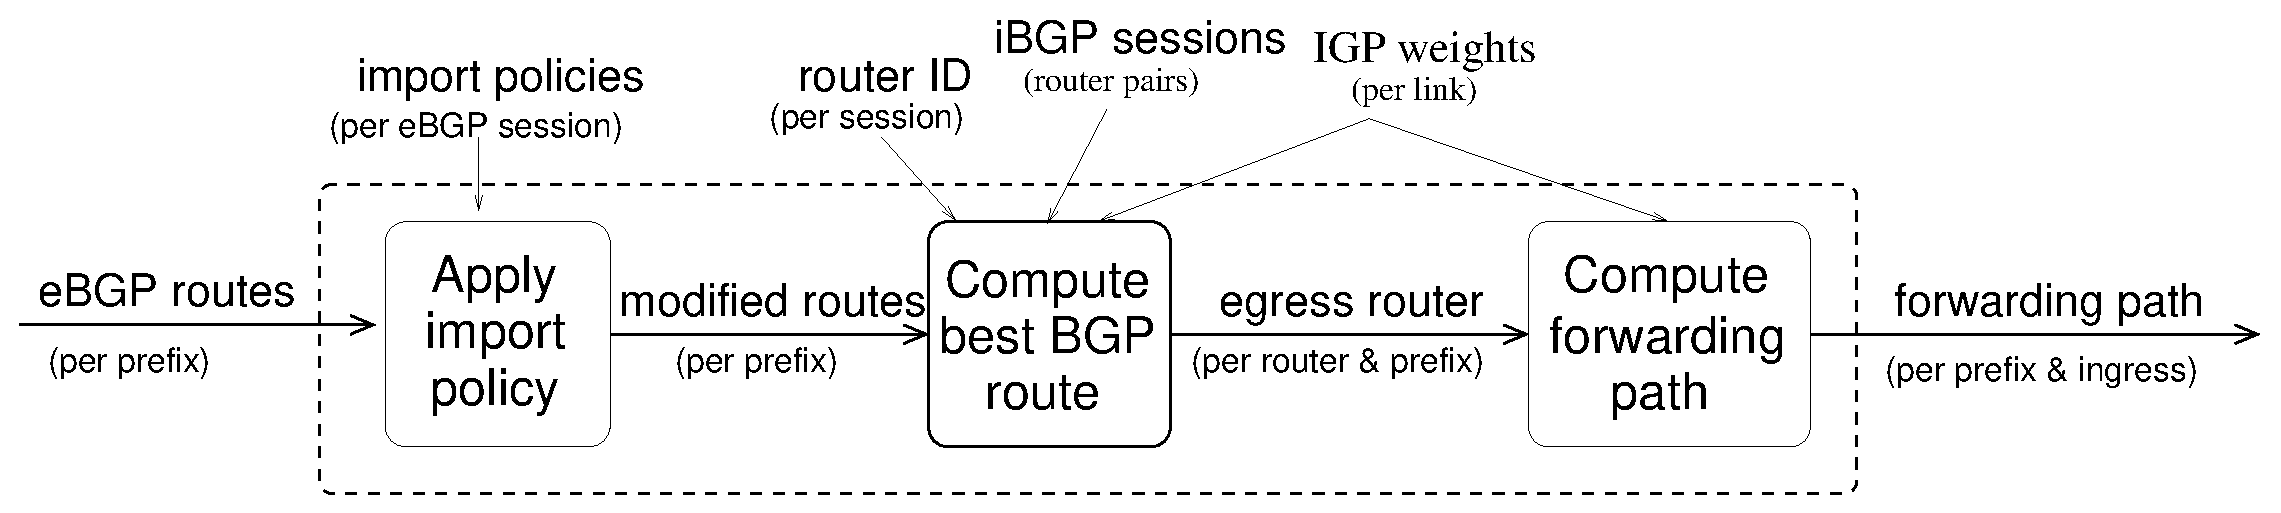
\epsfig{file=sandbox/figures/bigpic4.eps,width=\textwidth}
\caption[Decomposing BGP route selection into three
  independent stages.]{Our algorithms decompose network-wide BGP route
  selection into three independent stages.  The algorithms take as input
  the eBGP-learned routes from neighboring ASes, the router IDs of each
  BGP session, and the routing configurations from all of the routers in
  the AS, which provide information about the IGP topology, the iBGP
  topology, and the import policies (\ie, rankings) of each router.}
\label{fig:modules}
\end{figure*}

Following the approach applied in other recent
work~\cite{Feamster2005b,Gao2001a}, the algorithms in this chapter
compute the effects of a particular message ordering using an {\em
activation sequence\/}, an {\em offline} analysis technique that
``activates'' one or more routers at each discrete step.  When
activated, a router applies the decision process in
Table~\ref{tab:background:decision} and propagates the best route to its
iBGP neighbors.  Our algorithms are based on an activation sequence that
allows us to decompose route prediction into three distinct stages, as
shown in Figure~\ref{fig:modules}:

\textbf{1. Receiving the eBGP routes and applying import policy.} This
stage takes as input all of the eBGP-learned routes at each router and
applies the appropriate import policies at each router {\em before
exchanging any iBGP update messages} and outputs the set of eBGP-learned
routes after these import policies have been applied.  This stage
activates all of the edge routers at the same time.  

Each eBGP-learned route has attributes (such as the destination prefix
and the AS path) and is associated with an eBGP session.  The import
policy may filter the route or set certain attributes such as local
preference, origin type, and multiple-exit discriminator (MED),
according to attributes in the advertised route (\eg, based on ASes in
the AS path).  Because applying the import policy is a local operation
for each eBGP-learned route at each router, the first stage emulates the
operations a real router would perform upon receiving each of the eBGP
routes.  These routes, with modified attributes, are the input to the
second stage.

\textbf{2. Computing the best BGP route at each router.}  When iBGP
satisfies path visibility, many routes from the first stage could never
be selected by any router as the best route.  For example, an
eBGP-learned route with a local preference of 90 would {\em never} be
selected over another route with a local preference of 100.  In
addition, different routers in the AS may select different best BGP
routes because they have different IGP path costs to the egress router.
Also, a router can only consider the routes advertised by its iBGP and
eBGP neighbors, which may influence the final decision at that router.
%Deriving accurate and
%efficient algorithms for computing the best BGP route at each router
%is the main contribution of this paper.  
This stage takes as input the set of eBGP-learned routes after the
import policies of each router have been applied and outputs a single
best egress router for each ingress router and destination prefix.
Constructing an efficient activation sequence for this stage is
challenging, and is the focus of the next four sections of the chapter.

Using Observation~\ref{t:order}, our goal is to devise an {\em
activation sequence\/}, which ``activates'' one or more routers at any
given phase.  When activated, a router $r$ applies the BGP decision
process to compute a best route from its available candidate routes,
which it then may propagate to other routers via iBGP.  In an actual
network, routers may be activated in any order and may change their best
route many times before the network converges.  This chapter focuses on
devising activation sequences that allow us to efficiently compute
the final routing decision.


\textbf{3. Computing the forwarding path through the AS:} The third
stage of the algorithms compute the effects of the IGP link weights on
the construction of the forwarding path through the AS from an ingress
router toward a destination prefix.  Given the selected BGP route, the
ingress router forwards packets along the outgoing link (or links) along
shortest paths to the egress router, and the process repeats at the next
router.  Ideally, the traffic flows along the shortest path (or paths)
all the way from the ingress router to the selected egress router.
However, in practice, routers along the shortest path may have selected a
{\em different} egress router, thus violating route validity
(Definition~\ref{defn:rv}).  These 
violations can occur if the iBGP session configuration limits the
BGP routing options at the routers~\cite{Griffin2002}.  By considering
one router at a time, the third stage can compute an accurate view of
the forwarding path(s) even when deflections occur.

While all three steps are necessary for determining the flow of traffic
through a network from a static snapshot of the network state, the rest
of this chapter focuses on the second step (\ie, computing the best BGP
route at each router), since performing this step correctly and
efficiently is considerably more difficult than either of the other two
steps.

\input{sandbox/prediction}
\input{sandbox/implementation}
\section{Proposed Improvements to BGP}\label{sec:discussion}

Thus far, this chapter has focused on predicting BGP route selection
inside a single AS.  Notably, two artifacts, the MED attribute and route
reflection, complicate this process.  Not only do these attributes make
route prediction difficult, {\em they also create problems with the
  operation of 
BGP itself}.  The use of MED, both with and without route reflection has
been shown to cause oscillation~\cite{Basu2002}; route reflection can
also prevent convergence and cause forwarding loops~\cite{Griffin2002}.
The MED attribute is intended to allow a neighboring AS to dictate
preferred exit points on routes advertised at multiple exit points, but
it prevents a router from forming a consistent ordering of preferences
over routes.  Route reflectors were introduced to allow an iBGP topology
to scale, but they do so in a way that prevents routers from 
discovering the complete set of eBGP-learned routes.  

In this section, we explore possible solutions to the problems
introduced by MED and route reflection.  A major lesson one should draw
from this section is that a system that had visibility into an AS's
topology, configuration, and available BGP routes could actively {\em
control} the BGP route selection process, rather than simply trying to
predict its outcome.  The Routing Control Platform
(RCP)~\cite{caesar2004,feamster:fdna2004}, whose design we will 
discuss in Chapter~\ref{chap:concl}, can thus not only help
ensure correctness (as discussed briefly in
Section~\ref{sec:rcc_lessons}), but also make Internet routing easier to
control (and, hence, predict).

\subsection{MED-ication for Late-Exit Semantics}\label{sec:sandbox:med_disc}


The MED attribute causes problems because it is not comparable across
routes from different neighboring ASes, which prevents a router from
producing a consistent total ordering over all possible routes.  Also,
in networks without route reflection, inconsistent
preferences between pairs of routes is based on the router ID attribute,
an arbitrary tiebreak that carries no meaningful semantics (as in
Figure~\ref{fig:med}, for example).  

Before we consider solutions to the problems introduced by MED, it is
worth noting that MED, as it operates today and when used with
route reflection {\em may not have the intended effect on route selection}.
Consider the example shown in Figure~\ref{fig:ibgp2}.  A neighboring AS
sending routes $a$ and $b$ with MED values $10$ and $20$, respectively,
expects that the AS shown would always prefer route $a$ over route $b$,
as long as both existed, causing router $X$ to perform late-exit routing
(\ie, send its traffic via route $b$ via router $Y$).  Unfortunately,
the AS shown will {\em not} do so: $RR$ prefers route $c$, so router $X$
will never learn route $b$, and it will continue to forward packets via
route $a$.

We observe that if MED values are {\em remapped} into an explicit
ranking across neighboring ASes, rather than arbitrary values, then the MED
attribute 
{\em can} be compared across all routes at step~4 of the route selection
process (as it is today).  Comparing an exit-rank across
all routes can sometimes result in different outcomes than BGP today,
but in many cases the differences do not affect the important semantics
of BGP.  For example, consider Figure~\ref{fig:med}, but where the MED
attribute is compared across all routes.  Suppose that the route
selection process retains the MED comparison step, but that AS 2's MED
values of $10$ and $20$ are remapped to $1$ and $2$, and that the
highest MED value of any eBGP-learned route, $2$, is added to the MED
value on every route learned via iBGP (this transformation guarantees
that comparing MEDs across all routes would not cause iBGP-learned
routes to be preferred over eBGP-learned routes).  In this case, routers
$X$ and $Y$ would ultimately select routes $c$ and $d$, respectively, as
opposed to $a$ and $d$ in BGP today.  Although $X$ selects $c$ instead
of $a$, its preference between these two routes was based on the
arbitrary router ID tiebreak; therefore, having router $X$ select $c$
instead does not destroy any meaningful semantics.

The type of remapping we have described preserves MED's semantics,
%(as opposed MED's operation today, which provides no such guarantee),
but implementing an exit-rank requires visibility into the set of
available routes that is not available today.  Unfortunately, MED values
are typically based on dynamic values (\eg, IGP path costs across the
network), so an AS that sends routes with MED values cannot simply
configure a static 
ranking.  Given today's architectures, neither the sending nor receiving
AS could perform a remapping of MED values into an exit-rank, since no
single router learns the complete set of routes advertised from a
neighboring AS.  Performing such a remapping would require either the
sending or receiving AS to have complete visibility over all routes
being sent or received for a destination.  On the other hand, the
Routing Control Platform (RCP)~\cite{feamster:fdna2004} or similar
recently proposed architectures~\cite{id-versatile-rr} can perform such
a remapping, since RCP has full visibility of routes sent from a
neighboring AS (as well as full control over the routes that it sends to
a neighboring AS).
%
This modification allow the algorithm from Figure~\ref{fig:b2_tot_order}
to correctly compute 
the outcome of BGP route selection, and it would also eliminate intra-AS
safety problems.


\subsection{Scalability without Route Reflection} 

%% \begin{figure}[t]
%% \centering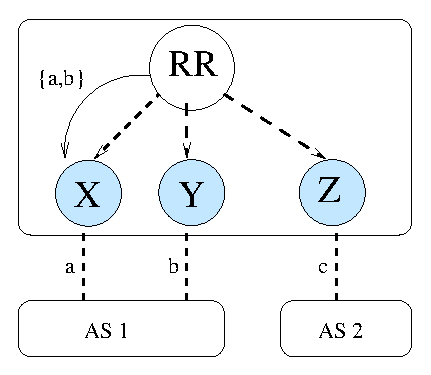
\epsfig{file=sandbox/figures/deflect.eps,width=0.45\linewidth}
%% \caption{Previous solutions~\protect\cite{Basu2002} to the MED
%%   oscillation problem can cause deflections and loops in some cases.  If
%%   $RR$ selects route $b$ but sends both $b$ and $c$ to router $X$, then
%%   $X$ might select route $c$ (\eg, for traffic engineering reasons,
%%   such as offloading traffic to AS 2).  However, packets forwarded from
%%   $X$ to $RR$ will still use $RR$'s best route $b$.}
%% \label{fig:deflect}
%% \end{figure}


Route reflectors allow iBGP topologies to scale to large number of
routers because they obviate the need to have a ``full mesh''
topology with $O(|R|^2)$ sessions. Unfortunately, they restrict route
visibility 
because they only send a single best route from all of the routes they
have learned.  In this chapter, we have explained how this restriction
complicates predicting the outcome of BGP route selection; previous work
has also 
noted that it can cause persistent oscillation and forwarding
loops~\cite{Basu2002, Griffin2002}.   

To remedy the problems with persistent oscillation, Basu {\em et al.}
proposed that route reflectors forward {\em all routes} that are equally
good up to and including the MED comparison.  It turns out that this
modification correctly emulates a full mesh iBGP topology; thus, it is
possible to model the outcome of their modified protocol with the
algorithm from Figure~\ref{fig:b2_no_tot_order}.  
Unfortunately,
this proposal
% has two significant drawbacks.  First, 
requires modifications to the routers, since each router readvertises
multiple routes instead of a single best route.  Additionally, because
each router readvertises multiple routes to its neighboring routers,
every router must select routes using a {\em consistent} selection criterion.
Otherwise, given multiple routes, some router along the path to an egress
router might select a different route, violating route
validity (Definition~\ref{defn:rv}).  This 
restriction precludes certain policies and configurations (\eg, a
router may not manipulate attributes on a route learned via iBGP).

%% Second, having a route
%% reflector advertise multiple routes while forwarding packets only on the
%% locally best route can cause deflections in circumstances where not all
%% routers along the path to an exit router select the same route.
%% Consider Figure~\ref{fig:deflect}.  Suppose $RR$ selects route $b$ and
%% sends routes $b$ and $c$ to router $X$.  Also assume that router $X$
%% prefers route $c$ over route $b$; such a situation could occur, for
%% example, if (1)~a network operator explicitly lowered the local
%% preference of routes from AS $1$ on router $X$ to offload some traffic
%% on that link, or (2)~the router ID tiebreak at router $X$ selects route
%% $c$.  If $X$ prefers $c$ over $b$, but its path to $Z$ traverses $RR$,
%% then $RR$ will forward packets intended for route $c$ via route $b$
%% instead. 

Architectures such as RCP propose separating route selection from the
routers and placing this functionality in a system that computes routes
on behalf of all of the routers within an AS~\cite{feamster:fdna2004}.
Rather than returning only a single best route to all of its clients (as
a route reflector does), RCP advertises to each router {\em the route
that it would have selected in a full mesh iBGP configuration}.  This
architecture allows the network to scale in the same way that route
reflectors do, but it provides some important additional advantages.
First, because RCP explicitly assigns routes to all routers in the
network, it can {\em guarantee} that the route assignments satisfy route
validity.  Second, RCP allows for a more 
scalable network design.  Furthermore, RCP does not have to make the
same routing decisions as its clients (as route reflectors do today).
As a result, unlike route reflectors, RCP nodes can be replicated at
arbitrary places in the IGP topology.


%%%
%%% conclusions.tex
%%%

\section{Summary}
\label{sec:sandbox_concl}

To perform everyday network engineering tasks effectively, efficiently,
and with minimal unnecessary changes to the live network, 
operators need a way to predict the behavior of a routing protocol
before deploying that configuration.  
%The model we have presented is a necessary step for advancing the state
%of the art of network engineering.
%, because it allows network operators (and protocol designers) to {\em
%reason} about BGP's behavior, rather than blindly tweaking the
%protocol with no understanding of the complex dynamics and protocol
%interactions.  
This chapter has presented route prediction algorithms that predict the
outcome of BGP route selection based on only a static snapshot of the
network state.

In addition to helping network operators accomplish traffic engineering
tasks, these algorithms provide useful insight into the subtleties of
network-wide BGP route selection and suggest several directions for
improvements to the Internet routing system.  For instance,
network-wide BGP route prediction could be combined with traffic
measurements to help network operators select BGP configuration changes
that achieve various traffic engineering goals.  In addition, the
emulator could be combined with higher-level mechanisms that spot
misconfiguration or check that other constraints
are satisfied~\cite{Feamster2004h}.

Although the diagram in Figure~\ref{fig:modules} shows only three
stages, we envision that network operators could incorporate other
phases.  For example, another phase could
combine the predicted forwarding paths with traffic data to predict
the load on each link in the network.  Using the model for traffic
engineering assumes that traffic volumes are relatively stable, and
that they remain stable in response to configuration changes.  In
previous work, we found that prefixes responsible for large amounts of
traffic have relatively stable traffic volumes over long
timescales~\cite{Feamster2003e}.  Operators could use the routing model to
test configuration changes on reasonably slow timescales that affect
prefixes with stable traffic volumes.  A network operator could also
combine measurements or estimates of the traffic arriving at each
ingress router for each destination prefix~\cite{Feldmann2001b} with the
link-level paths to predict the load on each link in the network.
Another phase might evaluate the optimality of the these link-level
paths in terms of propagation delay or link utilization and could
search for good configuration changes before applying them on a live
network.

Finally, we note that modeling BGP routing is more difficult than
it should be.  In the future, we hope that routing protocol designers
will consider predictability as a design goal; as we describe in
Section~\ref{sec:discussion}, some of these simplifications that aid
protocol modeling also fix problems with protocol {\em operation}.
Routing protocols that are easy to model and reason about will make
everyday network engineering tasks more tractable.


%% The prototype depends on many inputs including router 
%% configuration files, BGP table dumps, and BGP session information 
%% for every BGP-speaking router in the AS.  In reality, operators may not 
%% have access to all of these inputs, and some inputs may be incomplete 
%% or out-of-date.  Producing approximate results in the absence of  
%% complete information is a promising area for future work.

%In this section, we describe how
%operators can improvise in the face of incomplete or missing inputs.
%% The import policy application module relies on router configuration
%% files and a priori knowledge of what updates will be advertised via eBGP
%% from neighboring AS's.  Because the latter is impossible to know, we
%% approximate this using the externally learned routes in the BGP table
%% dumps (including alternate routes).  When some, but not all, routing
%% tables are available, it may be possible to approximate the missing
%% routing tables given knowledge of the other routing tables.  For
%% example, one simplifying assumption that may be valid for many networks
%% is to assume that all eBGP-speaking routers hear the same routing
%% advertisements.  \textbf{XXX how valid is this assumption?}


\section{Route Validity Faults}\label{sec:validity}

BGP should satisfy {\em route validity}, as defined formally in
Chapter~\ref{chap:rlogic} (Definition~\ref{defn:rv}).
%BGP configuration affects which routes each router accepts, selects, and
%readvertises.  
Table~\ref{tab:rcc_tests} summarizes the route validity faults that \rcc
checks.  The biggest challenge for checking route validity is
that the definition says that the routes the routers in an AS select
should induce only policy-conformant paths (see
Definition~\ref{defn:pcp}), but \rcc operates without a specification of
the intended policy.  This section focuses on \rccns's approach to
detecting potential policy-related problems.

Requiring operators to provide a high-level policy specification would
require designing a specification language and convincing operators to
use it, and it provides no guarantees that the results would be more
accurate, since errors may be introduced into the specification itself.
Instead, \rcc forms {\em beliefs} about a network operator's intended
policy in two ways: (1)~assuming that intended policies conform to best
common practice and (2)~analyzing the configuration for common patterns
and looking for deviations from those patterns.  (The idea of forming
beliefs about intended protocol behavior is inspired from similar ideas
in systems~\cite{Engler01}.)  \rcc then finds cases
where the configuration appears to violate these beliefs.  It is
noteworthy that, even in the absence of a policy specification, this
technique detects many meaningful configuration faults and generates few
false positives.

%% An AS's customers will sometimes advertise smaller prefixes to its upstream
%% AS to load balance its inbound traffic, but it will tag those prefixes
%% with an instruction to its upstream to not readvertise these
%% prefixes~\cite{rfc1997}.  The export policies on an AS's routers should
%% always ensure that such a route is not readvertised to any neighbors.
%% Network operators also control the export of routes between
%% their peers and providers.  Static analysis can check this property by
%% analyzing the configuration files to verify that every eBGP session has
%% a filter that matches routes that have this instruction and prevents
%% them from being readvertised to other ASes.

\subsection{Violations of Best Common Practice}

We can derive some notions of high-level policy from our knowledge of
best common practice (\ie, the manner in which many ASes
tend to configure their 
networks).  In particular, \rcc looks for two violations of best common
practice: (1)~advertising a route from one ``peer'' to another (\ie, a
violation of the common business practices defined in
Table~\ref{tab:business} (Section~\ref{sec:semantics}); and (2)~not
advertising routes in a consistent manner at all peering
points~\cite{Feamster2004b}.  In this section, we explain both of these
practices in more detail.

A route that an AS learns from one of its ``peers'' should not be
readvertised to another peer.  Checking this condition requires
determining how a route propagates through an AS.
Figure~\ref{fig:policy_closure} illustrates how \rcc performs this
check.  Suppose that \rcc is analyzing the configuration from AS $X$ and
needs to determine that no routes learned from AS $B$ are exported to
AS $A$.  First, \rcc determines all routes that AS $X$ exports to AS $A$,
typically a set of routes that satisfy certain constraints on their
attributes. For example, router $R_1$ may export to AS $A$ only routes
that are ``tagged'' with the label ``$1000$''.  As described in
Section~\ref{sec:conf}, ASes often assign such ``community'' labels to a
route to
control how other routers rank or filter it. \rcc then checks the {\em
import} policies for all sessions to AS $B$, ensuring that no import
policy will set route attributes on any incoming route that would place
it in the set of routes that would be exported to AS $A$.  To perform
this check, \rcc must know which of an AS's neighboring ASes are peers;
thus, this check requires this additional input from the network
operator.

Additionally, an AS should advertise routes with equally good attributes
to each peer at every peering point.  An AS should not advertise routes
with inconsistent attributes, since doing so may prevent its peer from
implementing ``hot potato'' routing:
If ASes $1$ and $2$ are
peers, then the export policies of the routers in AS $1$ should export
routes to AS $2$ that have equal AS path length and MED values.  If not,
router $X$ could be forced to send traffic to AS $1$ via router $Y$
(``cold potato'' routing).
This behavior typically violates peering
agreements.  Recent work has observed that this type of inconsistent
route advertisement sometimes occurs in practice~\cite{Feamster2004b}.

An AS's policies may violate this best common practice for two reasons.
First, an AS may apply different export policies at different routers to
the same peer.  Checking for consistent export involves comparing export
policies on each router that has an eBGP session with a particular peer.
Static configuration analysis is useful because it can efficiently
compare policies on 
many different routers.  In practice, this comparison is not
straightforward because differences in policy definitions are difficult
to detect by direct inspection of the distributed router configurations.
\rcc facilitates comparing export policies across sets of routers by
normalizing all of the export policies for an AS, as described in
Table~\ref{tab:if} (Section~\ref{sec:rcc_overview}).  Second, an iBGP
signaling partition can 
create inconsistent export policies because routes with equally good
attributes may not propagate to all peering routes.  For example,
consider Figure~\ref{f:ibgp_vis_violation} again.  If routers $W$ and
$Z$ both learn routes to some destination $d$, then route $W$ may learn
a ``better'' route to $d$, but routers $Y$ and $Z$ will continue to
select the less attractive route.  If routers $X$ and $Y$ readvertise
their routes to a peer, then the routes advertised by $X$ and $Y$ will
not be equally good.  Thus, \rcc also checks whether routers that
advertise routes to the same peer are in the same iBGP signaling
partition (as described in Section~\ref{sec:visibility}, \rcc checks for
all iBGP signaling partitions, but ones that cause inconsistent
advertisement are particularly serious).

\subsection{Configuration Anomalies}

\begin{figure}
\begin{center}
\begin{psfrags}
\psfrag{AS A}{AS $A$}
\psfrag{AS B}{AS $B$}
\psfrag{AS X}{{\LARGE AS $X$}}
\psfrag{R1}{$R_1$}
\resizebox{0.85\textwidth}{!}{\includegraphics{rcc/figures/policy_closure.eps}}
\end{psfrags}
\end{center}
\caption{How \rcc computes route propagation.}
\label{fig:policy_closure}
\end{figure}

When the configurations for sessions at different routers to a
neighboring AS are the same except at one or two routers, the deviations
are likely to be mistakes.  This test relies on the belief that, if an
AS exchanges routes with a neighboring AS on many sessions and most of
those sessions have identical policies, then the sessions with slightly
different policies may be misconfigurations.  Of course, this test could
result in many false positives because there are legitimate reasons for
having slightly different import policies on sessions to the same
neighboring AS (\eg, outbound traffic engineering), but it does provide
a useful sanity check.

%% that all
%% routes received from a peer look equally good up to the IGP tiebreak
%% step, thus allowing it to use nearest exit (``hot potato'') routing with
%% its peers.  Of course, an AS cannot ensure that it receives AS paths of
%% equal length at all peering points with its peer, but it can take
%% precautions such as resetting the MED value on import and ensuring that
%% the local preference value is the same everywhere.  



\qchapter{\textit{Why does everyone talk about the past? All that counts is
  tomorrow's game.}\vskip 0.1in - Roberto Clemente}{Conclusion}
\label{chap:concl}

Despite the fact that communication on the Internet relies on correct
and predictable operation of the routing protocols, today's Internet
routing infrastructure is surprisingly fragile.  The behavior of
Internet routing depends heavily on how today's {\em de facto} standard
Internet routing protocol, BGP, is configured.  Although BGP's
configuration is precisely what allows operators to realize complex
economic and policy goals, the resulting ``programmability'' of the
protocol creates the potential for incorrect and unpredictable behavior.
This dissertation has presented {\em proactive} techniques for improving
the correctness and predictability of Internet routing.  In this
chapter, we briefly review the causes for incorrect and unpredictable
behavior.  After summarizing the contributions of this dissertation in
Section~\ref{sec:concl:contrib}, we return in
Section~\ref{sec:concl:lessons} to the lessons learned 
from this work (see Section~\ref{sec:lessons}) and
propose some possible steps forward based on these lessons.
%Section~\ref{sec:concl:security} 
%briefly discusses open questions related to Internet routing security
%(\ie, how to guarantee correct and predictable behavior in the face of
%adversaries), and 
Section~\ref{sec:final} concludes.

\section{Reasons for Correctness and Predictability Problems}

Routing on the Internet involves the interaction between tens of
thousands of independently operated networks, or autonomous systems
(ASes), each of which may have anywhere from one to hundreds of
independently configured routers.  Although a network operator
configures each router independently, the behavior of the protocol may in
fact depend on the configurations of multiple routers, as well as the
dependencies between these configurations.  These
inter-router dependencies make configuring a network of
routers akin to writing a very large distributed program.  In light of the
fact that, until now, there have been no tools or techniques to help
network operators reason about the configuration of the network {\em as
a whole}, it is not surprising that network operators make mistakes
configuring their routers.

Even if network operators could be assured that the protocol would
always behave ``correctly'', they would still have no assurance
regarding what would actually happen to traffic in response to a
particular routing configuration.  Various protocol artifacts (\eg, the
MED attribute and route reflection), as well as the interaction of BGP
with interior routing protocols make it hard to predict route
assignments and traffic flow.
As such, to determine the effects of a potential configuration change on
the flow of traffic (and, hence, to determine whether such a
configuration change meets traffic engineering goals), an operator
currently has no choice but to test that configuration change on a
running network.  

Additionally, the operation of Internet routing depends on the
interactions of configurations across multiple administrative domains,
but network operators typically do not have access to the
configurations of these neighboring domains.  As a result of this
opacity, a network operator has no way to guarantee that the policies
configured in his own network will not conflict with those in
neighboring networks; worse yet, that operator has no way to debug a
problem caused by conflicting configurations when one does arise.
For example, as described in Chapters~\ref{chap:rlogic}
and~\ref{chap:policy}, ASes with conflicting policies can 
violate 
safety: unlike a shortest paths routing protocol, policy-based routing
protocols may never converge to a stable outcome if the policies in
neighboring ASes conflict~\cite{Varadhan1996}.  

\section{Summary of Contributions}\label{sec:concl:contrib}

This dissertation posited that the complexity of routing protocol
configuration is a major 
impediment to 
correct and predictable Internet routing and has presented {\em
proactive} techniques for improving the correctness and
predictability of Internet routing.  These techniques are based on 
a rigorous correctness specification for routing, which we presented in
Chapter~\ref{chap:rlogic}.  This specification has three aspects:
route validity, path visibility, and safety.  Although we have explored
the correctness specification in the context of today's Internet routing
system, we hope that it will prove useful for evaluating the behavior of
any routing protocol, particularly ones involving complex routing
policies (\eg, modifications to or replacements for BGP). 

Using this correctness specification as a guide, we have developed tools
and techniques that allow a network operator to detect problems and
predict routing protocol behavior {\em before} the configuration is deployed by
analyzing the static configuration files of the routers within a single
AS.  In particular, we presented two such tools:

\begin{itemize}
\itemsep=-1pt
\item \rcc, presented in Chapter~\ref{chap:rcc}, detects faults in the router
configurations within a single 
AS (\ie, violations of route validity, path visibility) by
analyzing the static configuration files.  \rcc has been downloaded by
over seventy network operators to date and is available for download at
\url{http://nms.lcs.mit.edu/rcc/}.
%
\item The route prediction algorithms presented in
Chapter~\ref{chap:sandbox} (and the associated prototype, the {\em routing
sandbox}) allows an operator to determine which routes each router will
ultimately select, given only a static snapshot of the router
configuration and the routes learned via eBGP.  We developed a prototype
of this tool and determined that our route computation algorithms are
both accurate and fast enough to be used to compute routes for a large
tier-1 ISP. 
\end{itemize}

In addition to providing these tools to help network operators
configure the Internet routing system, we also derive the constraints
that each AS's 
rankings must be subject to in order for the global routing system to
satisfy safety, presuming that each AS
retains complete autonomy in how it specifies both rankings and filters
(Chapter~\ref{chap:policy}). 
While the constraints we derived could certainly be implemented in \rccns, it
turns out that they are too restrictive: guaranteeing safety under such
circumstances essentially requires that each AS constrain its rankings
to be consistent with shortest paths routing.  We also speculated on the
implications of these results for the design of future Internet routing
systems. 

\section{Moving Forward from the Lessons Learned}\label{sec:concl:lessons}

Some researchers have lamented the ``ossification'' of the Internet
routing system and have argued that it is difficult to have real impact in
this area~\cite{Peterson2004}.  Indeed, much networking research either
analyzes the problems with the routing system or proposes solutions that
work within (or around) the limitations of BGP.  Arguably, the growing
research interest in overlay networks reflects the community's general
frustration with the difficulty of effecting real, substantive change in
the Internet's underlying routing system.  However, fixing the routing
system is an important and challenging goal that the networking research
community needs to address.  We believe that there are many open and
{\em important} problems related to these challenges where networking
researchers can have impact.

We now revisit the lessons learned (Section~\ref{sec:lessons}) and
discuss possible steps forward in terms of the two philosophies posed at
the end of Chapter~\ref{chap:intro}: (1)~leaving the routing infrastructure
largely unchanged and focusing on tools and techniques to make the
existing infrastructure more correct and predictable; or (2)~modifying
the existing architecture and infrastructure so that it is inherently
more correct and predictable.  In addition to revisiting the lessons
from Section~\ref{sec:lessons}, in 
Section~\ref{sec:concl:security}, we consider imminent open problems in
Internet 
routing security (\ie, how to guarantee correctness and predictability
in the face of adversaries).

\subsection{Static configuration analysis detects many faults}

One of the important lessons to take away from our experience with \rcc
is that static configuration
analysis detects many faults in deployed routing configurations.  
Of course, this lesson also begs the question of identifying and
detecting the types of faults that
cannot be detected with static analysis alone.  In general, there appear to be many
classes of events that are of interest to network operators that will
not be apparent from static analysis alone but can nevertheless exploit 
static analysis to help network operators drill down on the source of an
observed problem:

\begin{itemize}
\itemsep=-1pt
\item {\bf Shifts in traffic flow.}  Operators can use existing
monitoring infrastructure and anomaly detection tools to help them
detect shifts in traffic flow, but identifying the cause of a traffic
shift typically requires knowledge of many factors, including the
configuration.  For example, to determine whether a traffic shift was
caused by a change in demand or a change in routing, an operator may
want to see how the routes advertised from neighboring ASes have
changed or determine whether the configuration has changed.
The techniques described in Chapter~\ref{chap:sandbox} can help determine
how these changes would likely affect the flow of traffic.
%
\item {\bf Contract violations.}  Statically detecting faults in one's own
network provides no guarantees that neighboring networks will behave
correctly or scrupulously.  In these cases, dynamic analysis is
critical, but static 
analysis also plays a crucial role in helping operators identify
perpetrators. For example, recent work has developed an algorithm to
detect inconsistent route advertisements from neighboring
ASes~\cite{Feamster2004b}; this technique exploits static 
analysis of import policies to discount cases where an apparent
inconsistent route advertisement was in fact caused by the AS's own
import policies.
%
\item {\bf Performance degradations.}  While
static analysis alone cannot detect performance degradations, it can
help detect (or eliminate) possible causes for these degradations.  For
example, the checks for path visibility in iBGP (\eg,
Theorem~\ref{thm:vis}) can help a network 
operator quickly determine the source of dropped packets and can also
eliminate some potential causes of the problem.  In the case of routing
failures that affect end-to-end performance, the fastest way to
determine that a problem exists in 
the first place is to observe the end-to-end performance of Internet
paths, but static analysis may still play a useful diagnostic role in
many cases.

\item {\bf Route instability.}
In other cases, such as protocol oscillation cause by interaction between
MED and route reflectors or by interaction of policies between ASes,
static analysis is only useful for determining whether a route
oscillation {\em might} happen.  Careful analysis of the routing
announcements themselves, in conjunction with analysis of local policies,
may help determine when such oscillations actually arise and merit
attention. 
%
\item {\bf Security problems.}  Static analysis can help defend against
some routing security problems (\eg, advertising private address space
into the public Internet), but detecting route hijacks or otherwise
invalid route announcements in general is a challenging problem.  
Real-time analysis and detection of suspicious routing
announcements will play an important role in Internet routing security.
%\item {\bf Configuration faults.}
\end{itemize}

Dynamic analysis may play an important complementary role in solving
each of these problems, but an important open question is recognizing
that, for each case, a different ``signal'' may be necessary.  Existing
work that analyzes traffic patterns for anomalies faces a somewhat less
challenging problem because the timeseries to analyze is obvious (\ie,
amount of traffic per unit time).  With routing, the timeseries is less
obvious.  For example, when is it appropriate to analyze number of
prefixes advertised per unit time versus the total number of prefixes
announced by an AS versus the AS path length of a prefix over time, and
what techniques are most appropriate for analyzing
these signals?

\subsection{Distributed configuration causes faults}

Because {\em distributed} configuration is responsible for many
configuration faults, a natural possible step forward is to consider
ways to configure the network from a single, centralized point.
Refactoring configuration in this fashion would allow a network operator
to configure the {\em network}, rather than configuring routers.  This
proposal seems appealing, but several challenges stand in its way:

\begin{itemize}
\itemsep=-1pt
\item What type of language should such a centralized scheme use?  
\item What types of techniques would network operators be most likely to
adopt?
\item How can the expression of high-level policies be separated from
the low-level mechanisms that implement those policies?
\end{itemize}


Approaches to fault detection fall into two general categories: those
that take the existing configuration languages as given and analyze
deployed configuration for faults (analysis), and those that try to
design higher-level constructs to automatically generate low-level
router configuration (synthesis).  Both approaches can benefit
from better configuration languages that more closely correspond to the
network operator's intent.  For example, analysis techniques could
greatly benefit if they could check the actual routing configuration
against a specification of the intended behavior of the routing
protocol.  Such a specification could serve as a high-level language for
automatically {\em generating} low-level configuration.

Most network operators are trained on existing configuration languages,
and learning a new process for configuring routers has a high cost.
This situation suggests that the best way to spur adoption would be to
design a configuration language that allows an operator to more easily
construct configuration fragments from templates, which could be
customized according to higher-level macros.

In some sense, these two questions are closely related: network
operators will most likely be willing to adopt a configuration language
that is similar to the ones they use today.  In light of this
propensity, one possible approach is to generate a system that gives an
operator the semblance of configuring each independent router but is, in
reality, a centralized system that is responsible for pushing
configuration to the routers but can automatically check for invariants
that must hold network-wide.  Such a system is actually not that
different from the \rcc paradigm: the main difference is that the
network would be checked {\em before} it is deployed on running routers
and the operator would alter configurations in a centralized repository,
rather than on the individual routers.  Once configuration were
centralized in this fashion, however, the system could recognize
commonalities (``design patterns'') that existed across various routers
and BGP sessions and assist an operator in automatically generating
these common configurations. 



\subsection{Safety + Autonomy $\Rightarrow$ Tight restrictions on
expressiveness}

Our results concerning safety in Chapter~\ref{chap:policy} suggest that,
if ASes are given both complete freedom to establish business contracts
(\ie, set filters) and complete autonomy (both reasonably design
requirements for the foreseeable future), then the only Internet routing
protocol that is guaranteed to converge on a fast timescale is one where
paths are ranked according to consistent path costs (\eg, shortest path
routing).  

This result suggests that, moving forward, future Internet routing
protocols should either: (1)~constrain rankings so that they are derived
from consistent path costs but still provide operators the
latitude they need to implement business relationships; (2)~relax
autonomy, designing the protocol in such a way that reveals the fact
that a policy conflict exists without divulging sensitive information;
or (3)~devise more reasonable constraints on filtering that might
permit more flexible rankings.
%
In any case, it is clear that the Internet routing protocol must
both converge on a fast timescale, for reasons of both performance and
diagnostics, and somehow make it possible for ASes to express
preferences over the next-hop AS to which they send traffic (and make it
possible to recognize whether such rankings conflict).
%

The work in this dissertation examines one end of this spectrum: that
is, we explore how expressiveness can rankings be, providing for
unlimited autonomy 
and unrestricted filters.  Our results suggest that, in this regime,
ASes have relatively little expressiveness over rankings, which implies
that exploring how to relax requirements such as autonomy may be
worthwhile.  In Section~\ref{sec:policy:conclusion}, we discussed
possible several future directions.  We now revisit the strawman
proposal for a new routing protocol that we proposed in
Section~\ref{sec:policy:implications} and pose some open questions
related to this proposal. 

Suppose that every edge in the inter-AS graph had a corresponding
weight, that the cost of a path was the sum of all inter-AS edge weights
from source to destination, and that each AS was required to prefer the
path with lowest path cost.  To give operators some
latitude in setting rankings, further suppose that each AS had the
freedom to set the edge weights for only those edges that were incident
to its own AS in the graph (\ie, those edges from it to the next-hop AS
towards the destination).   Now, we know that such a protocol is
guaranteed to converge on a fast timescale, because all rankings are based
on shortest paths routing.  On the other hand, this strawman proposal
introduces two obvious problems:

\begin{itemize}
\itemsep=-1pt
\item {\bf Potentially poor isolation.} When an inter-AS edge fails, an
operator might 
have to re-tune the weights on the edges incident to his AS to guarantee
that traffic will continue flowing through the chosen next-hop AS for
that destination.  Is it possible to either design a scheme that
automatically tunes these weights for the operator and is still
guaranteed to be stable or, alternatively, a way of setting edge weights
that is relatively robust to these types of failures?
\item {\bf Policy disputes.} This strawman proposal does not eliminate
policy disputes entirely; rather, it {\em moves} the policy disputes so
that the protocol oscillates on a slower timescale.  Of course, there is
another advantage to this 
slower-timescale oscillation, in that the policy dispute will be
apparent from the continually increasing path costs.  Can the Internet
routing infrastructure incorporate a protocol that automatically detects
these disputes and facilitates renegotiation of business relationships
to resolve them?
\end{itemize}



\subsection{Protocol design should consider correctness and
predictability}\label{sec:rcp} 


This dissertation focuses on techniques for improving correctness and
predictability within the current Internet routing architecture, but a
more fruitful approach in the long term is to design the routing
protocol or architecture with an eye towards
preventing incorrect and unpredictable behavior in the first place.
The routing architecture should be designed to explicitly
provide correct and predictable behavior. Correctness and predictability
should not depend on the routing protocol's configuration; rather, they
should be {\em intrinsic} to the protocol's design.


\subsubsection{Separate routing from forwarding}


Our work on detecting faults in router configuration suggests that many
router configuration faults result from distributed nature of the
configuration.  The configuration of some policies introduces
dependencies between the configurations of multiple routers: the correct
operation of a filter on one router may be based on a label that a
different router attaches to the route.  
%
Additionally, many of the problems with BGP's correctness and
predictability result from today's techniques for disseminating routes
within an AS (\ie, iBGP route reflection).  Existing techniques for
disseminating BGP routes were designed as scalable, easily deployable
extensions to BGP, but did not consider correctness or predictability as
first-order concerns.  Route reflectors~\cite{rfc2796} eliminate the
need for a full mesh between iBGP speakers, but they do not correctly
emulate a full mesh iBGP configuration and, as a result, may cause the
protocol to violate basic correctness properties, as described in
Chapter~\ref{chap:rlogic}.  
After first surveying some techniques that make minor modifications to
iBGP to improve correctness and predictability, we explore how more
radical modifications to iBGP---specifically, those that separate Internet 
routing from the individual routers---might help network operators and
protocol designers cope with the complexity of Internet routing's
techniques for achieving policy and scalability.

Previous work has suggested making small modifications to the way that
route reflectors advertise routes to guarantee various correctness
properties.  RFC 1863 proposed that route servers forward {\em all\/}
routes to clients, rather than just a single best
route~\cite{rfc1863} and suggested using an ``advertiser''
attribute to allow recipients to know who advertised the routes.  Basu
\ea proposed a small modification to guarantee safety: instead
of having route reflectors only a single route to their clients, this
work proposes that route reflectors
should advertise all routes that are equally good up to the MED step in
the selection process (Table~\ref{tab:background:decision},
Chapter~\ref{chap:related})~\cite{Basu2002}.  In
Chapter~\ref{chap:rlogic} (Section~\ref{sec:mesh}), we also note that a
similar modification 
would also guarantee route validity.  Work on
BGP scalable transport (BST) has proposed other changes to iBGP that prevent
oscillations~\cite{Jacobson2003}.  Unfortunately, because these
proposals require modifying BGP (which implies either convincing router
vendors to implement the change, effecting the change through a standards
body such as the Internet Engineering Task Force, or both), they have
not been widely adopted.

\begin{figure}
\centering
\subfigure[In a conventional iBGP topology, every router in the AS
participates in IGP and iBGP and selects routes independently.]{
\epsfig{file=figures/pre_rcp.eps, width=0.45\linewidth}}\hfill
\subfigure[RCP receives the iBGP routes and the IGP topology from the
routers in the AS and computes routes on behalf of every router in the
AS, and assigns those routes using
iBGP~\cite{feamster:fdna2004}.]{ 
\epsfig{file=figures/rcp.eps, width=0.45\linewidth}}
\caption[Overview of Routing Control Platform]{Overview of the Routing
Control Platform (RCP) architecture.}
\label{fig:rcp}
\end{figure}

Rather than modifying the deployed routing infrastructure, the functions
of Internet routing could reside in a separate system that gathers
information about the topology (\eg, via iBGP and IGP), computes the
route that each router should use on behalf of each router, and assigns
the appropriate route to each router.  The idea of having a control
system that is separate from the infrastructure that is responsible for
forwarding packets (\ie, the routers) is the central idea of the 
Routing Control Platform (RCP)~\cite{caesar2004,feamster:fdna2004}
(see Figure~\ref{fig:rcp}), as well as work on a ``more versatile
route reflector'' that computes different routing decisions on behalf of
its client routers~\cite{id-versatile-rr}.  The IETF ForCES working
group has also proposed a framework that separates an individual
network element into separate control and forwarding elements, which can
communicate over a variety of media (\eg, a backplane, Ethernet,
etc.)~\cite{forces-wg}.  The framework dictates that routing protocols
be implemented in the control elements~\cite{rfc3746}.

Because RCP has a view of the AS-wide iBGP and IGP topologies, it can
assign routes to each router in a way that guarantees that the routing
protocol satisfies various properties, such as those from the
correctness specification in Chapter~\ref{chap:rlogic}.  RCP may also
simplify routing configuration, because configuration can be done on an
AS-wide basis, rather than router-by-router.  Rather than implementing
these policies with specifications of mechanism that are distributed
across the routers themselves, RCP could allow an operator to specify a
policy {\em for the entire AS} and be agnostic to the mechanisms that
actually implement the policy on the routers themselves.  

Separating routing state from the routers can potentially introduce
additional robustness, scalability, speed, and consistency problems.  The RCP
architecture must address these challenges to be viable.  We have implemented
a preliminary prototype of RCP as an 
extension to Quagga~\cite{www-quagga} to examine the feasibility of
having RCP control route selection for all of the routers in a large
tier-1 ISP~\cite{caesar2004}.  To study the other feasibility issues, we
are presently implementing RCP as extensions to the XORP software
router~\cite{Handley2002}; we plan to make this prototype available to
the research community.

%\section{Preventing Faults in the First Place}\label{sec:rcp}
%
%%%%
%%% introduction.tex
%%%

%\subsection{Introduction}\label{sec:intro}



Internet routing protocol
functionality should be separated from the routers.  Stated somewhat glibly,
routing is too important and too complicated to be
left to today's routers!  IP ``routers'' should be
``lookup-and-forward'' switches, forwarding packets as rapidly as
possible without being concerned about path selection.  
A separate entity should be responsible for 
computing the best BGP paths on behalf 
of all the routers in a domain and disseminating the results to the
routers. 

%Routers should forward packets but should not be
%concerned with distributed path computation.  Rather, a single
%logically centralized entity should perform all route computation on
%behalf of the routers in a routing domain.


%%%% This para should say WHY we believe in our position (motivation)

Separating interdomain routing from the individual routers is one way to
cope with the increasing complexity of the routing system.
The growth of the Internet has introduced considerable complexity into
interdomain routing, as  
features have been added to BGP to support
more flexibility (\eg, new route attributes such as communities and
MED) and larger scale (\eg, route reflectors and route aggregation).
This complexity has made routing protocol
behavior increasingly unpredictable and error prone~\cite{Feamster2004h}.
Requiring the 
routers to perform complex path computation introduces the potential
for inconsistencies across routers, complicates the expression of
routing policy, and makes troubleshooting difficult.


\begin{figure}[t]
\centering\epsfig{file=rcp/figures/interas.eps, width=\linewidth}
\caption[A Routing Control Platform (RCP) for the Internet.]{A Routing
Control Platform (RCP) for the Internet.  Circles 
  represent conventional routers.}
\label{fig:interas}
\end{figure}

%%% 
%%% Enabling 
%%%
Instead, a separate {\em Routing Control Platform (RCP)} should have
the information needed to select routes for each router in a domain
(\eg, an AS) and exchange routing information with RCPs in other
domains.\footnote{We use the term ``RCP'' to refer to
both the architecture as a whole and to the specific instance of RCP
within a routing domain.}
Figure~\ref{fig:interas} illustrates this idea.
%The RCP exchanges routing information with other ASes and sends each
%router in the AS a route to use in constructing its local forwarding
%table.  
Each RCP could use a new way of selecting routes for each router
(rather than using today's unwieldy BGP decision process); RCPs 
could even exchange routes using an interdomain routing protocol other
than BGP.  By selecting routes on behalf of {\em all\/} routers in a
domain, RCP can avoid many internal BGP-related complications (\eg,
forwarding loops~\cite{Dube99} and signaling partitions~\cite{Feamster2004h}).
%
%We believe that separating interdomain routing functionality from
%individual routers will reduce the complexity of routing configuration
%and management.  
%In this paper, we will
%describe how a logically centralized 
This approach also facilitates traffic engineering, simpler and less
error-prone policy expression, more powerful diagnosis and
troubleshooting, more rapid deployment of protocol modifications and
features, enforceable consistency of routes, and verifiable
correctness properties.  
%
In contrast to previous approaches for centralizing interdomain routes
and policies at route servers~\cite{Govindan1998}, RCP also preserves
the autonomy of each AS for selecting paths and applying
policies.\footnote{RCP more closely resembles the
Network Control Point (NCP), introduced in the telephone network in the
early 1980s to simplify network management and support the rapid
introduction of new features (\eg, enhanced 1-800 service)~\cite{Horing82,Lawser82}.}

RCP's deployment path is as interesting
as the envisioned end state.  The deployment of RCP can proceed in
three stages, offering the following benefits to network operators as
RCP becomes more widely deployed:

\begin{enumerate}
\itemsep=-1pt
\item \textbf{Control over protocol interactions:} RCP customizes the
distribution of BGP routes within an AS by replacing internal BGP route
reflectors.  This stage does not require cooperation from
neighboring domains.  Because RCP has a complete view of the intra-AS
topology and selects routes on behalf of all routers in the domain, it
can prevent internal BGP routing anomalies and control 
traffic flow more directly.

\item \textbf{Network-wide path selection and policy:} By establishing
BGP sessions
directly with the routers in neighboring ASes, RCP can perform all
routing decisions for an AS, bypassing the BGP decision
process on the routers.  This approach simplifies configuration and allows an
AS to select routes based on high-level goals, rather than obscure
manipulation of BGP route attributes.

\item \textbf{Redefinition of inter-AS routing:} Using RCPs, rather than
routers, to exchange routes between ASes (as shown in
Figure~\ref{fig:interas}) enables the design of a new routing protocol
because interdomain routing is now separated from IP routers.  For
example, RCP can be used to implement a control overlay that selects
paths based on prices or performance statistics.
\end{enumerate}
\noindent
%% Each phase reduces management complexity
%% fosters innovation and is completely backwards compatible with existing
%% routers. 


In addition to providing substantial improvements over today's routing
architecture, RCP has a compelling deployment incentive (\ie, a
``tipping point''), so that an individual AS could deploy RCP and
still realize significant benefits.  Because the first two stages of
deployment substantially reduce management complexity for BGP routing
{\em within a single AS\/}, network operators have a compelling
incentive to deploy RCP regardless of whether other ASes do so.
%Many innovative ideas (\eg, QoS, multicast, IPv6) have not yet
%been widely deployed operational networks because deploying these
%services provides no return until other ASes also do so.
%We believe that effecting real change in
%the Internet routing architecture requires a ``tipping point''---a
%compelling incentive for an AS to migrate to a new approach
%independently of other ASes.
%%%
%%% Tipping point
%%%
%Routing within a large backbone network depends on external BGP (eBGP)
%to exchange routes with other ASes, internal BGP (iBGP) to propagate
%these routes inside the AS, and the IGP to select paths between the
%routers in the AS.
Managing routing configuration requires constant vigilance from
network operators.  Although network management systems can often
automate the most frequent tasks, working around and within the
constraints of the existing routing protocols makes these systems much
more complicated than necessary.  Additionally, the complexity of
modeling and managing the distributed configuration state in today's
routers has itself impeded the evolution of automated management
systems.  
%Simplifying the management of a single network provides an
%incentive for an AS to deploy RCP independently of other ASes.
%%%
%%% As few changes as possible
%%%
In addition, because it communicates routes to each router in the
AS using BGP, RCP is backwards compatible with existing routers; deploying
RCP requires no changes to router hardware and software, only to
router {\em configuration}.


%%%%
%%% strawman.tex
%%%


\subsection{Architectural Principles for Routing}\label{sec:principles}

%% In this subsection, we describe the challenges of managing BGP within a
%% backbone network. Managing intra-AS routing presents three primary
%% challenges: (1)~the outcome intra-AS routing
%% depends on interactions between multiple routing protocols,
%% (2)~operators have indirect control over BGP's behavior, and (3)~because
%% iBGP's routing decisions are decentralized, common network management
%% and diagnosis tasks become more difficult.  The rest of this subsection
%% surveys these problems in further detail.

%% Despite the aspects of BGP that introduce fundamental problems and
%% stifle innovation, little attention has focused on designing protocol
%% improvements that fix these problems.  This lack of attention is largely
%% due to the fact that today's routing architecture does not support
%% innovation.  In this subsection, we describe three architectural principles
%% that will help facilitate innovation in interdomain routing.  In the
%% process, we describe specific aspects of today's routing system that
%% violate these principles.

In this subsection, we present three architectural principles for
reducing interdomain routing complexity:

\begin{enumerate}
\itemsep=-1pt
% 1
\item The routing architecture must base its routing assignments
on a consistent view of routing state. 
% 2
\item The interfaces between the routing protocols must minimize
unexpected or unwanted interactions.
% 3
\item The interdomain routing mechanisms must
directly support flexible, expressive policies.
\end{enumerate}
Each paragraph in this subsection discusses one of these principles.
For each principle, we present a high-level rationale, followed
by specific examples of how today's interdomain routing architecture
violates the principle.  For each of these examples, we suggest how
adhering to the architectural principle helps solve the problem.

%% In this subsection, we propose several architectural principles for
%% interdomain routing, all of which are rooted in traditional systems
%% design arguments, with the following goals in mind: (1)~to enable
%% innovation by fostering a more open platform for interdomain routing;
%% and (2)~to mitigate complexity of the interdomain routing system in
%% order to make network management easier.  To make the deployment of an
%% extensible routing platform feasible, we must keep both
%% goals in mind; in particular, the latter goal is the ``tipping point''
%% that gives operators an incentive to deploy an architecture based on
%% these principles.

\paragraph{Compute Routes Using Consistent State}

Routing state and logic should be co-located with the system components
that are assigning routes.  The logical participants in an interdomain
routing protocol are the {\em ASes\/}, not the individual routers.  The
interdomain routing architecture should view each AS as a single
participant and base routing decisions on a network-wide view of
available routes and configuration state; the routers, on the other
hand, should forward data traffic without concern about how the routes
are computed.  The current interdomain routing system violates this
architectural principle in the following three ways:
%
%The network ``core'' should maintain as little state as possible and the
%intelligence in networks should exist at endpoints.  
%Although the original Internet routing architecture incorporated the
%spirit of the end-to-end argument, 

%This argument holds
%important lessons for interdomain routing.  
%Routing is a distributed program that assigns IP-level paths to each
%destination.  


%First, {\em placing the ``intelligence'' of the routing protocol in
%the routers themselves prevents experimentation with and rapid
%deployment of new features}.  Many of the features of the interdomain
%routing system have ended up in the hands of router vendors because,
%to date, the best (and, arguably, the only) place to add functionality
%to the network is in the routers themselves.  Unfortunately, because
%most innovation at the routing layer involves compliance with
%proprietary hardware and software, as well as the slow-moving
%standards process, innovations to the routing architecture have been
%incremental and difficult to deploy.  Router vendors often add
%functionality in response to requests for new features (such as
%route-flap damping or BGP communities).  Moving the routing protocol
%logic out of the routers to the extent possible would allow protocol
%designers and network operators to easily experiment with and quickly
%deploy protocol modifications, without being tied to router hardware
%and software development cycles.

{\bf Decomposing the routing configuration state across the routers
unnecessarily complicates policy expression}.  Although
distributing state to achieve scalability and reliability makes sense,
many aspects of configuration are not replicated, but rather {\em
decomposed} across routers.  
%This decomposition
%of policy across routers does not improve scalability or reliability,
%but complicates policy expression and makes configuration
%inconsistencies more likely.  
Configuration state should be logically
centralized because it simplifies policy expression without compromising
scalability or reliability.

\vspace{0.05in}
\noindent
{\em Problem:} Network operators must often implement high-level policies,
such as preventing routes learned from one AS from being advertised to
another.  Implementing this policy currently requires modifying the
configurations of multiple routers: the import policies must ``tag''
eBGP-learned routes appropriately, and the export policies of other
routers must filter routes with this tag when advertising to eBGP
neighbors.  

\vspace{0.05in}
\noindent
{\em Solution:} Defining routing policy on a network-wide basis would
obviate the need for this level of indirection.  A network-wide
configuration management entity could know the origin of all routes
based on the eBGP sessions that advertised them, which would allow
a direct expression of policies based on sessions.
\vspace{0.05in}

%Because complexity makes reasoning extremely
%difficult, operators may be less likely to modify configuration because
%they lack the ability to reason about high-level behavior and fear
%introducing mistakes into the configuration.
%Additionally, distributing configuration can introduce
%unnecessary dependencies that actually make the routing protocol more
%error-prone than it should be.  
%This complexity discourages makes operators reluctant to experiment with
%changes and improvements for fear of introducing unintended side effects
%or ``fixing something that isn't broken''.  
%Configuration state should
%be distributed when doing so enhances scalability or reliability;

{\bf Distributed path selection causes routing decisions at one router
  to depend on the configuration of other routers}.  Subtle
  configuration details
  affect the route that a router selects or whether that router learns a
  route at all.  Computing routes on a network-wide basis using a
  consistent view of routing state can reduce interdomain routing's
  dependencies on these subtle details.
%selection can both explicitly enforce correct operation and facilitate
%modeling of the protocol behavior.
%

\vspace{0.05in}
\noindent
{\em Problem:} 
Omitting a single iBGP
session in a full-mesh configuration can leave a router with no route
for certain destinations, even if the intradomain topology is connected.
Distributed path selection also makes 
predicting the effects of configuration changes on traffic
flow difficult~\cite{Feamster2004}. 

\vspace{0.05in}
\noindent
{\em Solution:} 
An entity that performs path assignment on behalf of all
routers could control path assignment to ensure that every router is
assigned a route for every destination.
%For example, consider
%Figure~\ref{fig:today}, which shows how eBGP, iBGP, and IGP
%interoperate.  A router that learns a route on an iBGP session will not
%readvertise that route to routers on other iBGP sessions because those
%routers should have heard the same route from the router that learned
%the route via eBGP; if the iBGP topology is configured such that the
%routers in the top-level of the route reflector are not fully meshed,
%iBGP may not propagate routes to every router in the AS.
%(Incorrect iBGP configuration can also cause routing loops and
%oscillations; we discuss this in Section~\ref{sec:layer}.) 
\vspace{0.05in}

{\bf Each router is unaware of the state at other routers; this lack of
  information may result in incorrect or suboptimal routing.}.
  Implementing BGP's many features on the routers makes these features
  difficult to reason about.  For example, replication of functionality
  that is intended to
  improve reliability can cause forwarding loops, and a feature intended
  to prevent routing instability can slow convergence.  A routing
  architecture should implement these features in a 
  module that has
  a complete view of the network state, rather than in the routers
  (each of which only has a partial view of network state); doing so
  would allow that module to ensure sensible, consistent network-wide
  route assignment and override any feature interactions that cause
  incorrect routing. 
%  Controlling these protocol interactions centrally also makes it much
%  easier to physically replicate the entity performing route
%  computation.

%
% route-flap damping
\vspace{0.05in}
\noindent
{\em Problems:} 
% MED
%As another example, BGP's MED attribute allows an AS to express
%preference for how its neighbor selects an egress point for sending
%traffic (\ie, ``cold-potato'' routing).  Because MEDs are
%compared only between routes learned from the same AS, a router cannot
%form a total ordering of routes, which can cause persistent route
%oscillation~\cite{Griffin2002}.
% RR replicas
A router typically has iBGP sessions to multiple
route reflectors to improve reliability.  When a route reflector
fails, protocol oscillation and forwarding loops can arise if the
second route reflector has a different view of the best routes.
Placing the two route reflectors close to each other reduces these
kinds of inconsistencies but introduces fate sharing (\ie, the risk of
shared failures). 
%On the other hand, we believe that 
As another example, BGP route flap damping suppresses
unstable routes that change frequently~\cite{rfc2439}.  Unfortunately,
sometimes a 
single failure can trigger many advertisements that can mistakenly
activate route flap damping~\cite{Mao2002}.  Network operators must work
backwards to select configuration parameters that prevent erroneous
damping.

\vspace{0.05in}
\noindent
{\em Solution:} 
An entity that performs route
computation using a consistent view of available routes and network
topology can be replicated using standard distributed 
systems algorithms. Unlike route reflectors, each replica would assign
the same route to each router, independently of its location in the
network.
A module with knowledge of the routes assigned to every router in the
AS could also detect when route changes are caused by path exploration and
avoid unnecessarily suppressing a route.

\vspace{0.05in}
%Whenever possible, routing-protocol functionality should be decoupled
%from the routers.  That is there is no fundamental reason why a
%separate, vendor-independent device could not choose paths on behalf
%of the routers.  We believe that much of the research community's
%affection for overlay networks comes from the desire to control
%Internet routing and the frustration that the IP routing architecture
%remains largely closed to innovation.  Separating the path-selection
%process from the routers would enable exactly the kind of
%experimentation enabled by overlays today, but with the hope of
%directly influencing the behavior of the {\em underlay\/} network.

%%XXX Mention vendor-specific configuration? XXX

%Allowing each router in the AS to perform path selection introduces a
%A participant in a dynamic routing protocol updates its path selection
%as available routes change.
%If the routing decisions at each router are coupled with
%the propagation of the routing messages themselves, inconsistent (and
%incorrect) paths can result as updates propagate.  

\paragraph{Control Routing Protocol Interaction}\label{sec:layer}

Dividing functionality into distinct modules with clear interfaces can
control complexity.  In the routing system, the {\em IGP\/} computes
paths between routers in an AS, {\em eBGP\/} computes paths between ASes,
and {\em iBGP\/} propagates eBGP-learned routes throughout an
AS.  At a higher 
layer, {\em overlay networks\/} route traffic along one or more end-host
hops, abstracting the IP substrate entirely.
%In this subsection, we argue that the process of network protocol design
%and operation should respect this layering.
%
%As shown in Figure~\ref{fig:today}, an AS's border routers use eBGP to
%exchange routes for global destinations with other ASes; we call the
%layer at which eBGP routes are exchanged the {\em eBGP layer}.  Each
%eBGP-speaking router uses iBGP to exchange routes for global
%destinations with other routers in its AS.  We will refer to the layer
%at which iBGP routes are exchanged the {\em iBGP layer}.  If one of
%these routers selects a route for some destination that it learned from
%another router via iBGP, it will forward packets for that destination to
%that other router using the IGP path.  We will refer to the layer at
%which routers forward packets within an AS as the {\em IGP layer}.
%
Unfortunately, the modules in today's
interdomain routing system interact in the following undesirable ways:

{\bf Hard-wired interactions between eBGP and the IGP constrain an
operator's control over path selection.}  Although the internal
topology should have some influence on BGP routing decisions (\eg, 
it allows nearest-exit routing), a
router's choice of egress point should be relatively insensitive to
small IGP changes.
%, but it should still use IGP
%information when it informs BGP route selection.
%% Although the
%% routing architecture should {\em enable\/} IGP path costs to influence
%% the BGP routing decision, the interaction between the IGP and eBGP
%% layers {\em should not be hard-wired\/}.
%A router may learn multiple routes to a destination over several iBGP 
%sessions.  That router then applies a {\em de facto}
%``decision process'' to select a single best route to a destination.
%One step in that decision process dictates that routes with lower cost
%IGP paths be preferred over routes with longer IGP paths to an exit
%point.  
%The interplay between BGP and IGP limits operator control in two ways:
%(1)~minor changes in IGP routing can cause disproportionate effects in
%BGP routing, and (2)~to effect changes in intra-AS routing for network
%engineering, network operators are often forced to adjust the interdomain
%protocol configuration.
%
%Despite the benefits of hot-potato routing, 
%This happens because the BGP path selection process introduces
%dependencies on the IGP, a layering violation.

\vspace{0.05in}
\noindent
{\em Problem:} 
The BGP decision process uses the IGP path cost to break
the tie between two ``equally good'' routes. Internal events, such as
link failures, planned maintenance, or traffic engineering often lead to
changes in the IGP path costs.  These IGP changes can cause a router to
change its best {\em BGP\/} route, causing abrupt, unwanted traffic
shifts~\cite{teixeira2004b}.  Additionally, an operator may sometimes {\em
want\/} to redirect traffic from one egress link to another.  Today,
this requires complex manipulation of the BGP import policies to make
some egress points less attractive than others~\cite{Feamster2003e}.

\vspace{0.05in}
\noindent
{\em Solution:} 
With better control over the interactions between eBGP and IGP, an
operator could directly assign new routes to some routers without changing
BGP routing policies.
\vspace{0.05in}

{\bf Inconsistencies between iBGP and IGP can cause
forwarding loops and route oscillation.}  Operators can test that
their iBGP configuration satisfies sufficient conditions for
correctness~\cite{Griffin2002}, but this 
approach is not robust because operators commonly misconfigure
iBGP~\cite{Feamster2004h}.  The routing architecture should
explicitly {\em enforce\/} correctness constraints.  

\vspace{0.05in}
\noindent
{\em Problem:}
An
iBGP route reflector selects and distributes one best BGP route for each
destination prefix.  As a result, the route-reflector clients do not
necessarily make the same BGP routing decisions as they would in a
full-mesh iBGP configuration.  In particular, a route reflector and
its clients may have different IGP path costs to the
egress routers, leading to different BGP routing decisions, as shown 
previously in Figure~\ref{fig:rr}. 
%A route reflector and its clients may have a different view of the IGP
%path costs, which could result in inconsistent paths to the same
%egress point.
These inconsistencies can lead to protocol oscillations or persistent
forwarding loops~\cite{Basu2002,Griffin2002,rfc3345} if a router
forwards a packet toward one egress point via a router that has
selected a BGP route with a {\em different} egress point.  These
``deflections'' can also cause the AS-level forwarding path to differ
from the BGP AS path, which can complicate debugging~\cite{Mao2003}.

\vspace{0.05in}
\noindent
{\em Solution:} 
Rather than being agnostic about IGP forwarding paths, the routing
architecture could use the available knowledge to explicitly enforce
consistency in router-level forwarding paths.
\vspace{0.05in}

%decision process, can cause persistent route oscillation if route
%reflectors and their clients are not configured
%correctly~\cite{Griffin2002b,rfc3345}.  Griffin {\em
%et al.} observed that iBGP and IGP suffer from {\em asymmetry}, where
%the path over which data travels (determined by the IGP) is not
%necessarily the reverse of the control traffic
%(determined by the iBGP signaling graph)~\cite{Griffin2002}.  Asymmetry
%between iBGP and IGP can cause loops or ``deflections'' (\ie, instances
%where the forwarding path does not match the path indicated by the
%corresponding route), because routers along the IGP
%path may not agree on the same route to a
%destination~\cite{Dube99,Griffin2002}. 

%The interactions between iBGP and IGP complicate route selection and
%router-level forwarding paths. Even if an operator could predict the
%route that each router selects for a destination, it is still often
%difficult to determine whether the path over which packets are forwarded
%will actually follow that route.  For example, although conventional
%wisdom holds that iBGP route reflection simulates the effects of a full
%mesh iBGP topology, route reflection does not in fact do this.  A route
%reflector effectively executes the BGP decision process on behalf of its
%clients {\em under the assumption that its clients would have selected
%the same best route}.  Thus, the route that a router selects depends on
%the configuration of the route reflector hierarchy.  Configuring the
%route reflector hierarchy to avoid persistent forwarding loops requires
%extreme care.
%
%Although following proposed configuration guidelines can mitigate the
%undesirable interactions between iBGP and IGP, these work\-arounds
%avoid the fundamental protocol design problems that must be addressed as
%part of a long-term solution.  Interactions between iBGP and IGP become
%more considerably complex as the number of routers in an AS increases.
%One way of mitigating this complexity is to divide a large AS into
%multiple smaller ASes (or ``confederations'') with fewer routers.
%However, each configuration must still use iBGP to propagate routes
%internally, and the resulting larger network now comprises multiple ASes
%which are subject to misconfigurations themselves.  Additionally,
%previous work has derived sufficient conditions that must exist for iBGP
%to converge to a stable, loop-free routing that correctly propagates
%routes~\cite{Griffin2002}, but the protocol does not explicitly enforce
%these conditions.
%Although this work
%presents a practical, immediate way to avoid certain iBGP correctness
%problems, 
%the sufficient conditions on routing configuration are merely
%The intra-AS routing protocol should be designed to {\em
%enforce} these correctness constraints and explicitly prevent unwanted
%interactions between routing layers.\footnote{Tunneling (expand this)
%(\eg, via MPLS or IP-in-IP encapsulation) prevents persistent
%forwarding loops because forwarding decisions within the AS are
%determined by tunnels, rather than destination-based routing.
%Essentially, this type of tunneling enforces a layer separation between
%iBGP and the intra-AS routing. XXX Doesn't solve everything.}

{\bf Interactions between overlay networks and the underlying
network can degrade performance}.  
Overlay networks measure end-to-end path performance and tune routing
at the edge of the network, but they typically lack (1)~detailed {\em
measurements\/} of traffic and routing that would help them make
better decisions and (2)~direct {\em control\/} over IP-layer
protocols and mechanisms. The routing architecture should provide the
information and control that overlays need via a well-defined
interface. 
%

\vspace{0.05in}
\noindent
{\em Problem:} 
Route control products~\cite{www-routescience,www-sockeye}
help multihomed ISPs select upstream routes for each destination,
whereas end-host overlays such as RON~\cite{Andersen01} circumvent
failures and congestion by directing traffic through an intermediate
host.
% why are they harmful
Because they lack complete information about routing and
traffic-engineering optimizations, these overlays sometimes increase
congestion and decrease the effectiveness of traffic engineering in the
underlay network~\cite{Qiu2003}, which can degrade user performance.

\vspace{0.05in}
\noindent
{\em Solution:} 
With more direct control, overlays could operate more efficiently (\eg,
by not sending the same traffic over congested links at the network
edge~\cite{Jannotti2002}).  With more information about routing
dynamics, overlays could
pre-emptively avoid some outages~\cite{Feamster2003}. 

%% A control overlay, with a node in each AS, could monitor the behavior of
%% the routing system and drive the selection of paths in the under
%% network.  With an appropriate interface, this control overlay could
%% provide invaluable support to conventional overlay networks.


%Overlays improve end-to-end path performance and increase routing
%flexibility, but giving overlays the appropriate interface to the IP
%layer can improve network performance further.  Rather than creating
%control loop interactions between overlays and IP routing, the network
%architecture could provide the overlay with some level of control over
%the IP layer path to a destination.  Conversely, the IP layer could
%take ``hints'' from the overlay about end-to-end path performance and
%incorporate this into path selection at the IP layer.


% {\em BGP confederations or separate ASes:} problem still exists in
%      each confederation or mini-AS (though maybe RRs can be avoided), and
%      you now have to model a multi-AS network.  (I need to read ``on being
%      the right size'').




\paragraph{Support Flexible, Expressive Policies}

%% <<<<<<< strawman.tex
%% When used appropriately, abstraction can mitigate the complexity in
%% complex systems.  

%% However, the indirection that interdomain routing employs actually
%% exposes complexity rather than hiding it.  BGP's configuration and
%% operation involves multiple levels of indirection, but the indirection
%% it uses serves to complicate the protocol by {\em exposing mechanism},
%% rather than abstracting these details.  An interdomain routing protocol
%% should allow operators to specify tasks at the appropriate level of
%% abstraction, in a way that hides the mechanistic details of the routing
%% protocol rather than exposing them.  Note that these problems are not
%% merely configuration problems but involve fundamental protocol design
%% principles.
%% =======

%Much of the complexity of interdomain routing comes from the need to
%support competing domains with complex, sometimes conflicting, policy
%goals.  In fact, 
The interdomain routing architecture must support flexible, expressive
policy.  The need for greater flexibility in selecting and exporting
routes has driven many of the extensions to BGP over the past fifteen
years, and we believe this trend is likely to continue.  Although BGP is
highly configurable, its operation is controlled by {\em indirect\/}
mechanisms that expose details rather than abstracting them.
Architectural simplifications and better abstractions can simplify
configuration languages and make policy specification simpler and more
expressive.  The following points illustrate why today's routing
architecture does not satisfy these goals:

%Complex systems often exhibit emergent properties and unintended side
%effects. For example, a feature that is added for a certain reason may
%interact with others in strange and unexpected ways.  To control these
%types of effects, system designers often apply {\em modularity}:
%dividing the components of a system into groups of components such that
%each group can be reasoned about independently.  Designers aim to divide
%a system into modules in a way that minimizes the number of
%interconnections between modules.  Modules then interact with each other
%and with the environment via well-defined interfaces.  BGP's design
%gives rise to feature interactions, unnecessarily exacerbating
%complexity.  BGP's configuration and operation involves multiple
%unnecessary levels of indirection, which complicate the protocol by {\em
%exposing mechanism}, rather than abstracting these details.  In the
%remainder of this subsection, we describe how BGP's design restricts
%flexibility and gives rise to complicated feature interactions.

{\bf BGP's mechanisms preclude the expression of certain policies
and make others difficult to express.}  Network operators influence the
outcome of the BGP decision process by configuring policies that modify
the attributes of BGP routes.  Better configuration languages would be
helpful, but the architecture should also provide more flexible support
for assigning paths to routers.  

\vspace{0.05in}
\noindent
{\em Problem:} 
Moving
traffic from one inter-AS link to another requires~\cite{Feamster2003e}:
(1)~identifying the subset of prefixes that carries the desired amount of
traffic, (2)~determining how to express that subset (\eg, by a common
AS path regular expression), (3)~modifying the import policies on one or
more routers to assign a smaller ``local preference'' for routes
matching those expressions, and (4)~observing the resulting traffic flow
and iterating as necessary.  

\vspace{0.05in}
\noindent
{\em Solution:} 
Although ``what if'' tools can help predict
the effects of policy changes~\cite{Feamster2004}, the routing architecture
should allow an operator to move traffic by {\em explicitly} assigning paths.

%% Additionally, BGP has a ``hold timer'' setting that
%% specifies how the router will wait in between BGP ``keepalive'' messages
%% before deciding that a session has failed.  The hold timer setting is an
%% indirect mechanism for expressing how fast a router should detect a
%% failure.  The setting of the hold timer is somewhat of an art: for
%% example, a short hold timer interval allows for quicker detection of
%% failed sessions, but the interval must be longer than IGP convergence
%% delay to prevent spurious session resets.

{\bf BGP's mechanisms impede multiple ASes from cooperating in
selecting routes that satisfy their goals.}  ASes must cooperate to
ensure end-to-end reachability, but today's routing architecture does
not directly support this type of cooperation.  Interdomain routing
policies are a tussle space~\cite{clark2002}: an AS must balance the
dependence on its neighbors for good connectivity to the rest of the
Internet and competition with neighbors for customers and revenue.
Operators must currently resolve these conflicts outside of the
infrastructure, but
the architecture should directly support route
selection based on negotiated preferences or financial incentives.

\vspace{0.05in}
\noindent
{\em Problem:} 
Suppose one AS wants to advertise a backup route to its
neighbor.  These two ASes must first negotiate a backup
``signal'' out of band.  The AS advertising the route must then modify
its export policies to attach this signal to the backup route, and the
neighbor must modify the import policies on its routers to lower
the ``local preference'' value for routes with this community.

\vspace{0.05in}
\noindent
{\em Solution:} 
Because route negotiation is fundamental to inter-AS
cooperation, the interdomain routing should support it directly. 

%Additionally, an
%upstream neighbor might have a strong preference for the second route
%but would not have an easy way to convey this interest.  Although such
%preferences could be conveyed out of band~\cite{mahajan2005}, each AS
%would need to reconfigure each router appropriately.


%% Finally, {\em router configuration languages dictate low-level
%% specification of protocol behavior, rather than high-level policy or
%% operator intent}.  Operators must express constraints on route
%% distribution using indirect methods of expression.  To do so, they
%% typically implement filters that control the distribution of routes
%% based on whether a route's attributes matches specified pattern.  For
%% example, an operator may configure a router to filter routes that have a
%% certain ``community'' attribute~\cite{rfc2519}.  Controlling route
%% propagation using communities involves definitions at three levels of
%% indirection: (1)~mapping a BGP session to the names of import and export
%% policies, (2)~mapping the name of each policy to a set of clauses, each
%% of which defines conditions for accepting or rejecting a route and
%% modifying route attributes, and (3)~defining various variables that are
%% used in the clause of a policy statement (\eg, specifying what AS
%% regular expression number $x$ refers to).  These levels of indirection
%% make controlling route distribution complicated and error-prone because
%% they specify {\em how} the protocol should implement a certain behavior,
%% rather than directly specifying the policy to implement.  A
%% protocol and configuration language that supported direct expression of
%% high-level policy would ease the burden of network management.
%  communities+ACLs for aggregation~\cite{rfc2519}
%  and imposing relationships like customer, peer, and provider

%An interdomain routing protocol should allow operators to specify tasks
%at the appropriate level of abstraction, in a way that hides the
%mechanistic details of the routing protocol rather than exposing them.
%Note that these problems are not merely configuration problems but
%involve fundamental protocol design principles.  Better router
%configuration languages would mitigate some of these problems, but many
%of the problems associated with this interface result from incorrect
%{\em protocol} mechanisms.  Thus, allowing operators to configure
%routers at the appropriate level of abstraction involves architectural
%changes, as well as improvements to the configuration language itself.







%\input{rcp/architecture}
%\input{rcp/weaknesses}
%

XXX remove
Scaling problems exist not only within a single AS, but also between
groups of ASes.  The route arbiter project proposed placing route
servers at exchange points~\cite{Govindan1998} to obviate the need for a
full mesh eBGP topology (\ie, at the exchange point) by applying policy
once at the route server.  This architecture facilitates centralized
application of BGP routing policies at a single exchange point.  In
Section~\ref{sec:rcp}, we present RCP, which primarily addresses how to
scalably disseminate routes {\em within} a single AS.  In some ways, RCP
can be viewed as an analog to route servers~\cite{Govindan1998} for
intra-AS route dissemination: whereas route servers were used to reduce
the number of eBGP sessions from $O(n^2)$ to $O(n)$, where $n$ is the
number of ASes at an exchange point, RCP reduces the number of iBGP
sessions from $O(n^2)$ to $O(n)$, where $n$ is the number of routers in
a single AS.  Because RCP separates the logic of route selection from
the physical routers, it is conceivable that it could also used as a
platform for developing new mechanisms for exchanging routes between
pairs or groups of routers. 


Ultimately, RCP can facilitate innovation because it allows the logic of
route selection to be located in a system that is separate from the
infrastructure that is responsible for forwarding data traffic.  Moving
routing into a logically centralized (albeit replicated) system creates
more flexibility in how routes are exchanged between RCP nodes in
neighboring ASes: RCP nodes in adjacent ASes could use BGP to exchange
these routes, 
although they could conceivably use any protocol.  RCP could also expose
more information about the routing topology to applications such as
overlay networks, as well as give these networks more control over the
IP-level routes that are actually used.

Moving routing functionality into a system like RCP is not the only way
to separate routing from forwarding: others have advocated removing
routing from the AS entirely by moving routing complexity to end hosts,
which query route servers to discover routes~\cite{Lakshminarayanan2004,
Yang2003}.  Although these projects share our goal of separating routing
complexity from the infrastructure, RCP has the added benefit of
simplifying intra-AS routing.  Recent work has also proposed working
around the existing infrastructure, using an overlay to improve BGP's
robustness~\cite{Agarwal2003, Goodell2003}.


\subsubsection{Provide direct control over traffic}

Much research, both in Chapter~\ref{chap:sandbox} and in previous
work~\cite{Feldmann2000}, has focused on developing predictive models of
network-wide routing, typically to assist network operators in traffic
engineering. A system like RCP can provide {\em real-time control\/} of
BGP routes rather than modeling the BGP routes in today's routing
system.  That is, rather than trying to infer the outcome of BGP route
selection or otherwise monitor the routing protocol (as many existing
systems do~\cite{www-ipsumnetworks,www-packetdesign, Shaikh2004}), RCP
can {\em control} the outcome, thus directly controlling how traffic
flows.

Although RCP provides direct control over traffic, it does not provide
any facilities for helping operators determine {\em how} that traffic
should be controlled.  Similarly, Chapter~\ref{chap:sandbox} presented
algorithms that help network operators predict the effects of
configuration changes on the flow of traffic through the network, but
these algorithms do not help network operators actually discover a
routing configuration that achieves their intended objective (\eg,
relieving persistent congestion, minimizing congestion on peering links,
etc.).  Unlike {\em intra}domain routing optimization, for which there
are existing tools and algorithms to help operators tune
parameters~\cite{www-cariden-mate,Feldmann2000}, {\em inter}domain routing is
much more difficult to optimize: the search space is much larger, and
local configuration changes can have global effects that alter the
traffic volumes coming {\em to} that AS from neighboring ASes.  Our
previous work proposes some guidelines for helping network operators
make configuration changes that are less likely to cause unpredictable
effects~\cite{Feamster2003e}, but the design techniques for efficiently finding
optimal (or even ``good'') configuration settings remain open.


\subsubsection{Avoid manipulable routing objects}

Recall from Chapter~\ref{chap:rlogic} that we considered a destination
$d$ to be an immutable ``handle'' for a route that referred to a set of
endpoints; we cited IP prefixes as the destination $d$ in
the case of Internet routing.  Unfortunately, prefixes are {\em not}
immutable: a router in one AS can {\em aggregate} IP prefixes that are
contiguous in 
the address space taking two routes, $(d_1 \rightarrow v_i)$ and $(d_2
\rightarrow v_j)$ and combining them into a single route, $(d
\rightarrow v_k)$, such that any packets destined for endpoints in
either $d_1$ or 
$d_2$ will be forwarded according to the route $(d\rightarrow v_k)$.
This creates complications for the definition of an induced path
(Definition~\ref{defn:ipath}), since a route to any endpoint by be
induced by routes for different destination handles at different
routers.

\begin{figure}
\centering\epsfig{file=figures/aggregate.eps, width=0.65\linewidth}
\caption[How aggregation can interfere with an AS's attempt to control
  inbound traffic.]{Aggregation can interfere with an AS's attempt to
  control inbound traffic.  In this example, AS~1 announces more
  specific routes to AS~3 in an attempt to have inbound traffic enter
  via that AS.  AS~3, on the other hand may aggregate (or simply filter)
  those more specific routes to save routing table space, thus
  interfering with AS~1's intent.}
\label{fig:aggregate}
\end{figure}

Not only do these manipulable routing objects create problems for reasoning
about properties of the routing protocol, but they also create practical
problems.  For one, they create a tension between control over inbound
traffic and scalability.  ASes typically exploit the fact that routers
will forward traffic based on the longest matching IP prefix in the routing
table and send more specific routing information along links where it
wishes to attract traffic.  This technique allows an AS to control how
traffic reaches its AS from 
other places on the Internet.  On the other hand, to control routing
table size, some ASes may combine multiple more specific routes into a
single shorter route using a process called aggregation.  Aggregation
dramatically reduces routing table size because Internet addressing is
typically hierarchical.  Unfortunately, aggregating more specific
prefixes can also interfere with an ASes attempt to control how traffic
reaches its network, as shown in
Figure~\ref{fig:aggregate}~\cite{id-path-validation}.  Thus, ASes must
either aggregate routes at the risk of interfering with the traffic
engineering goals of other ASes (the common practice
today~\cite{nanog-prefix-aggregation}) or maintain larger routing tables
without receiving compensation for the incurring the extra overhead.

Finally, recent work has observed that, because IP prefixes can be
manipulated by routers in other ASes, they often do not accurately
reflect a set of destinations 
that is atomically either reachable or
unreachable~\cite{Freedman2005}. This characteristic can cause
violations of route validity (Definition~\ref{defn:rv}) when a portion
of endpoints contained within some destination become unreachable but
the route advertising the IP prefix for those endpoints is not
withdrawn.

In light of these problems presented by aggregation, one reasonable
design principle for future Internet routing systems may be to make the
destination that is referred to by a route an 
immutable property of the route, as a recent proposal has
suggested~\cite{Vutukuru2005b}. 

%% Even if a router makes the same routing decision for two contiguous
%% prefixes, it typically cannot aggregate those routes because it does not
%% know if other routers that learn BGP routes from this router might
%% select different routes for the separate prefixes.  

%% AIP as possible answer?








\subsection{Consider the effects of adversaries on correctness
and predictability}
\label{sec:concl:security}

This dissertation addresses the challenges for correctness and
predictability that are introduced unintentionally.  A growing threat to
the Internet routing infrastructure, however, is that posed by
adversaries.  For example, malicious parties may attempt to inject false
routing information in an attempt to divert or blackhole traffic.
Routing security has been studied in some detail~\cite{perlman88}, but
{\em interdomain} routing security is particularly difficult because
interdomain routing must support complex policy.  In addition to
securing routing information, the infrastructure should also ultimately
provide guarantees about where the traffic actually goes---in other
words, whether the {\em induced path} (Definition~\ref{defn:ipath},
Chapter~\ref{chap:rlogic}) actually corresponds to the information about
the path that is carried in the route.


\subsubsection{Control-Plane Security}

Attacks against the control plane have received considerable attention
in recent years.  The IETF has established a working group in routing
protocol security, RPSEC~\cite{rpsec-wg}; recent drafts have addressed
threats to the Internet routing system and BGP and outlined security
requirements~\cite{id-routing-threats}.  BGP does not provide any
support for controlling route announcements.  Securing the control plane
boils down to two tasks: {\em origin authentication}, which verifies
that the AS that is announcing (``originating'') the prefix actually has
legitimate ownership over the address space for that prefix; and {\em
path authentication}, which verifies that the sequence of ASes that the
routing advertisement traversed corresponds to the sequence of ASes in
the AS path.

Various proposals provide either origin authentication~\cite{id-sobgp},
path authentication~\cite{Hu2004:spv}, or both~\cite{kent2000b}.
Unfortunately, these schemes require the existence of a public
key infrastructure (PKI), a central authority that manages key
distribution, ownership, and revocation; PKIs are cumbersome and
difficult to 
maintain.  Thus, developing a routing protocol that automatically
verifies the ownership of some address space without requiring a
centralized, trusted verification or lookup infrastructure remains an
important unsolved problem.

Even an Internet routing architecture that provides both origin and path
authentication still does not enable an AS to verify that the route it
receives is one that it {\em should be receiving}.  That is, while they
allow an AS to verify that a route announcement traversed a particular
sequence of ASes, they do not provide any mechanism to allow an AS to
verify that the sequence of ASes is one that is sensible.  Answering
this question is critical for routing security.  If an AS has no way to
determine whether a sequence of ASes is sensible, then it is possible
for a single malicious organization to establish a new AS and have that
AS buy transit from the upstream AS of a source and destination,
respectively.  An important unsolved problem involves characterizing the
types of bogus routes that an AS can detect with the limited information
available today, as well as determining the additional information that
should be added to the routing protocol that could assist this detection
without 
revealing sensitive business relationships.


\subsubsection{Data-Plane Security}

Even if an AS could verify that the routes it receives were authentic
and policy-compliant, it still has no way to verify that packets
actually traverse the same ASes as those in the route's AS
path~\cite{Mao2003}.  We note that the AS path was never intended as an
indication of the ASes that traffic will actually traverse.  Rather, the
AS path was only
ever intended for loop detection (\ie, so that an AS would not
readvertise a route that it had already learned) and as a coarse metric
for choosing shorter routes over longer ones.  Nevertheless, providing
some guarantees over where traffic will (or won't) travel appears to be
a desirable goal for Internet routing.  Allowing an AS or end host to
verify that a route's AS path matches the actual forwarding path, or,
more generally, allowing it to ascertain the sequence of ASes that
traffic to or from some destination traverses are important capabilities
that any future Internet routing system should provide.  

%% While restricting route propagation is a reasonable way to restrict
%% unwanted traffic, a malicious entity can always try to ``dump'' traffic
%% for a certain destination on any advertised link, in the hope that the
%% router will carry traffic to that destination anyway.  A router should
%% reject packets destined for hosts with no corresponding advertised
%% route.  More generally, a router should reject packets from sources that
%% should not have a valid route through this router to the destination.
%% Deploying packet filters only at routers in large ASes in the Internet
%% ``core'' could eliminate most of these packets~\cite{Park2001}, but an
%% AS must be able to construct these filters in the first place, which
%% would require discovering the routes from the source to that AS.
%% \begin{itemize}
%% \itemsep=-1pt
%% \item {\em Dynamic packet filter construction.} How can an AS
%%   determine the source and destination addresses it
%%   should see on packets arriving on a link?~\footnote{This
%%   question has a dual for {\em route\/} filters in the 
%%   control plane.} 
%% \end{itemize}


\section{Concluding Remarks}\label{sec:final}

%% Muse about how awesome the correctness specification is and how it can
%% be used to analyze all of these cool new features and additions.  Now,
%% it's just our job to come up with those features!

This dissertation has (1)~presented a correctness specification for
Internet routing; (2)~developed tools and techniques to check for
violations of this correctness specification in real-world routing
configuration; (3)~exploited the correctness specification to design
algorithms that predict the outcome of BGP route selection for the set
of routers within an AS; and (4)~derived the first conditions for
guaranteeing a {\em global} correctness property, safety, that do not
require global knowledge of business relationships or topology.  

The current version of the Internet's routing protocol, BGP, has been
deployed for nearly a decade and has been modified and extended numerous
times (\eg, with route reflection).  More striking is the plethora of
proposals that have not been deployed.  In light of these proposals, the
key challenge is to be able to separate the good protocol modifications
from the bad ones and to determine how these various modifications
interact with each other. 
The correctness specification presented in this dissertation facilitates
this type of reasoning. Furthermore, the proactive techniques that this
dissertation has advocated and developed can help resolve the tension
between flexibility and complexity that exists in any complex routing
protocol. 
%proposed routing 
%protocol (or even a modification to BGP, for that matter) will solve the
%problems it claims to solve without introducing new problems of its own.
While we have presented the properties of the correctness specification
in the context of BGP, it is our hope that this specification can serve
as a guide for both evaluating and designing new routing protocols that
explicitly provide correctness and predictability. 



\end{sloppypar}


%%%%%%%%%%%%%%%%%%%%%%%%%%%%%%%%%%%%%%%%%%%%%%%%%%%%%%%%%%%%


\begin{flushleft}
\bibliographystyle{abbrv}
\rhead[\fancyplain{}{}]{\fancyplain{}{\sfb\thepage}}
\lhead[\fancyplain{}{\sfb\thepage}]{\fancyplain{}{}}
\cleardoublepage
\rhead[\fancyplain{}{\sfeight\MakeUppercase{\bibname}}]{\fancyplain{}{\sfb\thepage}}
\lhead[\fancyplain{}{\sfb\thepage}]{\fancyplain{}{\sfeight\MakeUppercase{\bibname}}}
%\addcontentsline{toc}{chapter}{\bibname}
\bibliography{ref,rfc}

\end{flushleft}

\end{document}

